\PassOptionsToPackage{unicode=true}{hyperref} % options for packages loaded elsewhere
\PassOptionsToPackage{hyphens}{url}
%
\documentclass[]{book}
\usepackage{lmodern}
\usepackage{amssymb,amsmath}
\usepackage{ifxetex,ifluatex}
\usepackage{fixltx2e} % provides \textsubscript
\ifnum 0\ifxetex 1\fi\ifluatex 1\fi=0 % if pdftex
  \usepackage[T1]{fontenc}
  \usepackage[utf8]{inputenc}
  \usepackage{textcomp} % provides euro and other symbols
\else % if luatex or xelatex
  \usepackage{unicode-math}
  \defaultfontfeatures{Ligatures=TeX,Scale=MatchLowercase}
\fi
% use upquote if available, for straight quotes in verbatim environments
\IfFileExists{upquote.sty}{\usepackage{upquote}}{}
% use microtype if available
\IfFileExists{microtype.sty}{%
\usepackage[]{microtype}
\UseMicrotypeSet[protrusion]{basicmath} % disable protrusion for tt fonts
}{}
\IfFileExists{parskip.sty}{%
\usepackage{parskip}
}{% else
\setlength{\parindent}{0pt}
\setlength{\parskip}{6pt plus 2pt minus 1pt}
}
\usepackage{hyperref}
\hypersetup{
            pdftitle={Codes for STEM},
            pdfauthor={Noushin Nabavi},
            pdfborder={0 0 0},
            breaklinks=true}
\urlstyle{same}  % don't use monospace font for urls
\usepackage{color}
\usepackage{fancyvrb}
\newcommand{\VerbBar}{|}
\newcommand{\VERB}{\Verb[commandchars=\\\{\}]}
\DefineVerbatimEnvironment{Highlighting}{Verbatim}{commandchars=\\\{\}}
% Add ',fontsize=\small' for more characters per line
\usepackage{framed}
\definecolor{shadecolor}{RGB}{248,248,248}
\newenvironment{Shaded}{\begin{snugshade}}{\end{snugshade}}
\newcommand{\AlertTok}[1]{\textcolor[rgb]{0.94,0.16,0.16}{#1}}
\newcommand{\AnnotationTok}[1]{\textcolor[rgb]{0.56,0.35,0.01}{\textbf{\textit{#1}}}}
\newcommand{\AttributeTok}[1]{\textcolor[rgb]{0.77,0.63,0.00}{#1}}
\newcommand{\BaseNTok}[1]{\textcolor[rgb]{0.00,0.00,0.81}{#1}}
\newcommand{\BuiltInTok}[1]{#1}
\newcommand{\CharTok}[1]{\textcolor[rgb]{0.31,0.60,0.02}{#1}}
\newcommand{\CommentTok}[1]{\textcolor[rgb]{0.56,0.35,0.01}{\textit{#1}}}
\newcommand{\CommentVarTok}[1]{\textcolor[rgb]{0.56,0.35,0.01}{\textbf{\textit{#1}}}}
\newcommand{\ConstantTok}[1]{\textcolor[rgb]{0.00,0.00,0.00}{#1}}
\newcommand{\ControlFlowTok}[1]{\textcolor[rgb]{0.13,0.29,0.53}{\textbf{#1}}}
\newcommand{\DataTypeTok}[1]{\textcolor[rgb]{0.13,0.29,0.53}{#1}}
\newcommand{\DecValTok}[1]{\textcolor[rgb]{0.00,0.00,0.81}{#1}}
\newcommand{\DocumentationTok}[1]{\textcolor[rgb]{0.56,0.35,0.01}{\textbf{\textit{#1}}}}
\newcommand{\ErrorTok}[1]{\textcolor[rgb]{0.64,0.00,0.00}{\textbf{#1}}}
\newcommand{\ExtensionTok}[1]{#1}
\newcommand{\FloatTok}[1]{\textcolor[rgb]{0.00,0.00,0.81}{#1}}
\newcommand{\FunctionTok}[1]{\textcolor[rgb]{0.00,0.00,0.00}{#1}}
\newcommand{\ImportTok}[1]{#1}
\newcommand{\InformationTok}[1]{\textcolor[rgb]{0.56,0.35,0.01}{\textbf{\textit{#1}}}}
\newcommand{\KeywordTok}[1]{\textcolor[rgb]{0.13,0.29,0.53}{\textbf{#1}}}
\newcommand{\NormalTok}[1]{#1}
\newcommand{\OperatorTok}[1]{\textcolor[rgb]{0.81,0.36,0.00}{\textbf{#1}}}
\newcommand{\OtherTok}[1]{\textcolor[rgb]{0.56,0.35,0.01}{#1}}
\newcommand{\PreprocessorTok}[1]{\textcolor[rgb]{0.56,0.35,0.01}{\textit{#1}}}
\newcommand{\RegionMarkerTok}[1]{#1}
\newcommand{\SpecialCharTok}[1]{\textcolor[rgb]{0.00,0.00,0.00}{#1}}
\newcommand{\SpecialStringTok}[1]{\textcolor[rgb]{0.31,0.60,0.02}{#1}}
\newcommand{\StringTok}[1]{\textcolor[rgb]{0.31,0.60,0.02}{#1}}
\newcommand{\VariableTok}[1]{\textcolor[rgb]{0.00,0.00,0.00}{#1}}
\newcommand{\VerbatimStringTok}[1]{\textcolor[rgb]{0.31,0.60,0.02}{#1}}
\newcommand{\WarningTok}[1]{\textcolor[rgb]{0.56,0.35,0.01}{\textbf{\textit{#1}}}}
\usepackage{longtable,booktabs}
% Fix footnotes in tables (requires footnote package)
\IfFileExists{footnote.sty}{\usepackage{footnote}\makesavenoteenv{longtable}}{}
\usepackage{graphicx,grffile}
\makeatletter
\def\maxwidth{\ifdim\Gin@nat@width>\linewidth\linewidth\else\Gin@nat@width\fi}
\def\maxheight{\ifdim\Gin@nat@height>\textheight\textheight\else\Gin@nat@height\fi}
\makeatother
% Scale images if necessary, so that they will not overflow the page
% margins by default, and it is still possible to overwrite the defaults
% using explicit options in \includegraphics[width, height, ...]{}
\setkeys{Gin}{width=\maxwidth,height=\maxheight,keepaspectratio}
\setlength{\emergencystretch}{3em}  % prevent overfull lines
\providecommand{\tightlist}{%
  \setlength{\itemsep}{0pt}\setlength{\parskip}{0pt}}
\setcounter{secnumdepth}{5}
% Redefines (sub)paragraphs to behave more like sections
\ifx\paragraph\undefined\else
\let\oldparagraph\paragraph
\renewcommand{\paragraph}[1]{\oldparagraph{#1}\mbox{}}
\fi
\ifx\subparagraph\undefined\else
\let\oldsubparagraph\subparagraph
\renewcommand{\subparagraph}[1]{\oldsubparagraph{#1}\mbox{}}
\fi

% set default figure placement to htbp
\makeatletter
\def\fps@figure{htbp}
\makeatother

\usepackage{booktabs}
\usepackage[]{natbib}
\bibliographystyle{plainnat}

\title{Codes for STEM}
\author{Noushin Nabavi}
\date{2020-09-19}

\begin{document}
\maketitle

{
\setcounter{tocdepth}{1}
\tableofcontents
}
\hypertarget{coding-for-stem}{%
\chapter{Coding for STEM}\label{coding-for-stem}}

\begin{quote}
Tools and capabilities of data science is changing everyday!
\end{quote}

This is how I understand it today:

\textbf{Data can:}
* Describe the current state of an organization or process\\
* Detec anomalous events\\
* Diagnose the causes of events and behaviors\\
* Predict future events

\textbf{Data Science workflows can be developed for: }\\
* Data collection and management\\
* Exploration and visualization\\
* Experimentation and prediction

\textbf{Applications of data science can include: }\\
* Traditional machine learning: e.g.~finding probabilities of events, labeled data, and algorithms\\
* Deep learning: neurons work together for image and natural language recognition but requires more training data\\
* Internet of things (IOT): e.g.~smart watch algorithms to detect and analyze motion sensors

\textbf{Data science teams can consist of:}
* Data engineers: SQL, Java, Scala, Python\\
* Data analysts: Dashboards, hypothesis tests and visualization using spreadsheets, SQL, BI (Tableau, power BI, looker)\\
* Machine learning scientists: predictions and extrapolations, classification, etc. and use R or python * Data employees can be isolated, embedded, or hybrid

Data use can come with risks of identification of personal information. Policies for personally identifiable information may need to consider:\\
* sensitivity and caution\\
* pseudonymization and anonymization

Preferences can be stated or revealed through the data so questions need to be specific, avoid loaded language, calibrate, require actionable results.

\textbf{Data storage and retrieval may include: }
* parallel storage solutions (e.g.~cluster or server)\\
* cloud storage (google, amazon, azure)\\
* types of data: 1) unstructured (email, text, video, audio, web, and social media = document database); 2) structured = relational databases\\
* Data querying: NoSQL and SQL

\textbf{Communication of data can include: }\\
* Dashboards\\
* Markdowns\\
* BI tools\\
* rshiny or d3.js

\textbf{Team management around data can use: }
* Trello, slack, rocket chat, or JIRA to communicate due data and priority

\textbf{A/B Testing: }
* Control and Variation in samples\\
* 4 steps in A/B testing: pick metric to track, calculate sample size, run the experiment, and check significance

Machine learning (ML) can be used for time series forecasting (investigate seasonality on any time scale), natural language processing (word count, word embeddings to create features that group similar words), neural networks, deep learning, and AI.\\
\textbf{Learning can be classified into: }
\emph{Supervised}: labels and features/ Model evaluation on test and train data with applications in:
* recommendation systems\\
* subscription predictions\\
* email subject optimization\\
\emph{Unsupervised}: unlabeled data with only features\\
* clustering

\textbf{Deep learning and AI requirements: }
* prediction is more feasible than explanations\\
* lots of very large amount of training data

\hypertarget{introduction}{%
\chapter{Introduction}\label{introduction}}

Importing data into R

working with excel, csv, txt, and tsv files in R

\begin{Shaded}
\begin{Highlighting}[]
\KeywordTok{library}\NormalTok{(readr) }
\KeywordTok{library}\NormalTok{(data.table)}
\KeywordTok{library}\NormalTok{(readxl)}
\KeywordTok{library}\NormalTok{(gdata)}
\CommentTok{# library(XLConnect)}
\KeywordTok{library}\NormalTok{(httr)}
\KeywordTok{library}\NormalTok{(rvest)}
\KeywordTok{library}\NormalTok{(xml2)}
\KeywordTok{library}\NormalTok{(rlist)}
\KeywordTok{library}\NormalTok{(jsonlite)}
\KeywordTok{library}\NormalTok{(dplyr)}
\end{Highlighting}
\end{Shaded}

Importing csv file:
pools \textless{}- read.csv(``swimming\_pools.csv'', stringsAsFactors = FALSE)

With stringsAsFactors, you can tell R whether it should convert strings in the flat file to factors.

Import txt file with read.delim:
hotdogs \textless{}- read.delim(``hotdogs.txt'', header = FALSE)

Import txt file with read.table:
hotdogs \textless{}- read.table(path,
sep = ``\t",
col.names = c(''type``,''calories``,''sodium"))

Import with readr functions:
- read\_csv, read\_tsv, and read\_delim are part of this package

Can specify column names before import:
properties \textless{}- c(``area'', ``temp'', ``size'', ``storage'', ``method'',
``texture'', ``flavor'', ``moistness'')

Import potatoes.txt:
potatoes \textless{}- read\_tsv(``potatoes.txt'', col\_names = properties)

Import potatoes.txt using read\_delim():
potatoes \textless{}- read\_delim(``potatoes.txt'', delim = "\t", col\_names = properties)

Import 5 observations from potatoes.txt:
potatoes\_fragment \textless{}- read\_tsv(``potatoes.txt'', skip = 6, n\_max = 5, col\_names = properties)

Import all data, but force all columns to be character: potatoes\_char
potatoes\_char \textless{}- read\_tsv(``potatoes.txt'', col\_types = ``cccccccc'', col\_names = properties)

Import without col\_types
hotdogs \textless{}- read\_tsv(``hotdogs.txt'', col\_names = c(``type'', ``calories'', ``sodium''))

The collectors you will need to import the data
fac \textless{}- col\_factor(levels = c(``Beef'', ``Meat'', ``Poultry''))
int \textless{}- col\_integer()

Edit the col\_types argument to import the data correctly:
hotdogs\_factor \textless{}- read\_tsv(``hotdogs.txt'',
col\_names = c(``type'', ``calories'', ``sodium''),
col\_types = list(fac, int, int))

Import potatoes.csv with fread() from data.table:
potatoes \textless{}- fread(``potatoes.csv'')

Import columns 6 and 8 of potatoes.csv:
potatoes \textless{}- fread(``potatoes.csv'', select = c(6, 8))

Plot texture (x) and moistness (y) of potatoes:
plot(potatoes\(texture, potatoes\)moistness)

Print the names of all worksheets using readxl library:
excel\_sheets(``urbanpop.xlsx'')

Read the sheets, one by one
pop\_1 \textless{}- read\_excel(``urbanpop.xlsx'', sheet = 1)
pop\_2 \textless{}- read\_excel(``urbanpop.xlsx'', sheet = 2)
pop\_3 \textless{}- read\_excel(``urbanpop.xlsx'', sheet = 3)

Put pop\_1, pop\_2 and pop\_3 in a list:
pop\_list \textless{}- list(pop\_1, pop\_2, pop\_3)

Read all Excel sheets with lapply():
pop\_list \textless{}- lapply(excel\_sheets(``urbanpop.xlsx''), read\_excel, path = ``urbanpop.xlsx'')

Import the first Excel sheet of urbanpop\_nonames.xlsx (R gives names):
pop\_a \textless{}- read\_excel(``urbanpop\_nonames.xlsx'', col\_names = FALSE)

Import the first Excel sheet of urbanpop\_nonames.xlsx (specify col\_names):
cols \textless{}- c(``country'', paste0(``year\_'', 1960:1966))
pop\_b \textless{}- read\_excel(``urbanpop\_nonames.xlsx'', col\_names = cols)

Import the second sheet of urbanpop.xlsx, skipping the first 21 rows:
urbanpop\_sel \textless{}- read\_excel(``urbanpop.xlsx'', sheet = 2, col\_names = FALSE, skip = 21)

Print out the first observation from urbanpop\_sel
urbanpop\_sel{[}1,{]}

Import a local file
Similar to the readxl package, you can import single Excel sheets from Excel sheets to start your analysis in R.

Import the second sheet of urbanpop.xls:
urban\_pop \textless{}- read.xls(``urbanpop.xls'', sheet = ``1967-1974'')

Print the first 11 observations using head()
head(urban\_pop, n = 11)

Column names for urban\_pop
columns \textless{}- c(``country'', paste0(``year\_'', 1967:1974))

Finish the read.xls call
urban\_pop \textless{}- read.xls(``urbanpop.xls'', sheet = 2,
skip = 50, header = FALSE, stringsAsFactors = FALSE,
col.names = columns)

Import all sheets from urbanpop.xls
path \textless{}- ``urbanpop.xls''
urban\_sheet1 \textless{}- read.xls(path, sheet = 1, stringsAsFactors = FALSE)
urban\_sheet2 \textless{}- read.xls(path, sheet = 2, stringsAsFactors = FALSE)
urban\_sheet3 \textless{}- read.xls(path, sheet = 3, stringsAsFactors = FALSE)

Extend the cbind() call to include urban\_sheet3: urban\_all
urban \textless{}- cbind(urban\_sheet1, urban\_sheet2{[}-1{]}, urban\_sheet3{[}-1{]})

Remove all rows with NAs from urban: urban\_clean
urban\_clean \textless{}- na.omit(urban)

Print out a summary of urban\_clean
summary(urban\_clean)

When working with XLConnect, the first step will be to load a workbook in your R session with loadWorkbook(); this function will build a ``bridge'' between your Excel file and your R session:
Here using the XLConnect package

Build connection to urbanpop.xlsx:
my\_book \textless{}- loadWorkbook(``urbanpop.xlsx'')

List the sheets in my\_book
getSheets(my\_book)

Import the second sheet in my\_book
readWorksheet(my\_book, sheet = 2)

Import columns 3, 4, and 5 from second sheet in my\_book: urbanpop\_sel
urbanpop\_sel \textless{}- readWorksheet(my\_book, sheet = 2, startCol = 3, endCol = 5)

Import first column from second sheet in my\_book: countries
countries \textless{}- readWorksheet(my\_book, sheet = 2, startCol = 1, endCol = 1)

cbind() urbanpop\_sel and countries together: selection
selection \textless{}- cbind(countries, urbanpop\_sel)

Add a worksheet to my\_book, named ``data\_summary''
createSheet(my\_book, ``data\_summary'')

Use getSheets() on my\_book
getSheets(my\_book)

Create data frame:
sheets \textless{}- getSheets(my\_book){[}1:3{]}
dims \textless{}- sapply(sheets, function(x) dim(readWorksheet(my\_book, sheet = x)), USE.NAMES = FALSE)
summ \textless{}- data.frame(sheets = sheets,
nrows = dims{[}1, {]},
ncols = dims{[}2, {]})

Add data in summ to ``data\_summary'' sheet
writeWorksheet(my\_book, summ, ``data\_summary'')

Rename ``data\_summary'' sheet to ``summary''
renameSheet(my\_book, ``data\_summary'', ``summary'')

Remove the fourth sheet
removeSheet(my\_book, 4)

Save workbook to ``renamed.xlsx''
saveWorkbook(my\_book, file = ``renamed.xlsx'')

Download various files with download.file()
Here are the URLs! As you can see they're just normal strings:

\begin{Shaded}
\begin{Highlighting}[]
\NormalTok{csv_url <-}\StringTok{ "http://s3.amazonaws.com/assets.datacamp.com/production/course_1561/datasets/chickwts.csv"}
\NormalTok{tsv_url <-}\StringTok{ "http://s3.amazonaws.com/assets.datacamp.com/production/course_3026/datasets/tsv_data.tsv"}

\CommentTok{# Read a file in from the CSV URL and assign it to csv_data}
\NormalTok{csv_data <-}\StringTok{ }\KeywordTok{read.csv}\NormalTok{(}\DataTypeTok{file =}\NormalTok{ csv_url)}

\CommentTok{# Read a file in from the TSV URL and assign it to tsv_data}
\NormalTok{tsv_data <-}\StringTok{ }\KeywordTok{read.delim}\NormalTok{(}\DataTypeTok{file =}\NormalTok{ tsv_url)}

\CommentTok{# Examine the objects with head()}
\KeywordTok{head}\NormalTok{(csv_data, }\DataTypeTok{n =} \DecValTok{2}\NormalTok{)}
\end{Highlighting}
\end{Shaded}

\begin{verbatim}
##   weight      feed
## 1    179 horsebean
## 2    160 horsebean
\end{verbatim}

\begin{Shaded}
\begin{Highlighting}[]
\KeywordTok{head}\NormalTok{(tsv_data, }\DataTypeTok{n =} \DecValTok{2}\NormalTok{)}
\end{Highlighting}
\end{Shaded}

\begin{verbatim}
##   weight      feed
## 1    179 horsebean
## 2    160 horsebean
\end{verbatim}

Download the file with download.file()

\begin{Shaded}
\begin{Highlighting}[]
\KeywordTok{download.file}\NormalTok{(}\DataTypeTok{url =}\NormalTok{ csv_url, }\DataTypeTok{destfile =} \StringTok{"feed_data.csv"}\NormalTok{)}

\CommentTok{# Read it in with read.csv()}
\NormalTok{csv_data <-}\StringTok{ }\KeywordTok{read.csv}\NormalTok{(}\DataTypeTok{file =} \StringTok{"feed_data.csv"}\NormalTok{)}


\CommentTok{# Add a new column: square_weight}
\NormalTok{csv_data}\OperatorTok{$}\NormalTok{square_weight <-}\StringTok{ }\NormalTok{(csv_data}\OperatorTok{$}\NormalTok{weight }\OperatorTok{^}\StringTok{ }\DecValTok{2}\NormalTok{)}
\end{Highlighting}
\end{Shaded}

Save it to disk with saveRDS()
saveRDS(object = csv\_data, file = ``modified\_feed\_data.RDS'')

Read it back in with readRDS()
modified\_feed\_data \textless{}- readRDS(file = ``modified\_feed\_data.RDS'')

Using data from API clients

example 1
Load pageviews library for wikipedia

\begin{Shaded}
\begin{Highlighting}[]
\KeywordTok{library}\NormalTok{(pageviews)}

\CommentTok{# Get the pageviews for "Hadley Wickham"}
\NormalTok{hadley_pageviews <-}\StringTok{ }\KeywordTok{article_pageviews}\NormalTok{(}\DataTypeTok{project =} \StringTok{"en.wikipedia"}\NormalTok{, }\DataTypeTok{article =} \StringTok{"Hadley Wickham"}\NormalTok{)}

\CommentTok{# Examine the resulting object}
\KeywordTok{str}\NormalTok{(hadley_pageviews)}
\end{Highlighting}
\end{Shaded}

\begin{verbatim}
## 'data.frame':	1 obs. of  8 variables:
##  $ project    : chr "wikipedia"
##  $ language   : chr "en"
##  $ article    : chr "Hadley_Wickham"
##  $ access     : chr "all-access"
##  $ agent      : chr "all-agents"
##  $ granularity: chr "daily"
##  $ date       : POSIXct, format: "2015-10-01"
##  $ views      : num 53
\end{verbatim}

Load the httr package:

\begin{Shaded}
\begin{Highlighting}[]
\KeywordTok{library}\NormalTok{(httr)}

\CommentTok{# Make a GET request to http://httpbin.org/get}
\NormalTok{get_result <-}\StringTok{ }\KeywordTok{GET}\NormalTok{(}\DataTypeTok{url =} \StringTok{"http://httpbin.org/get"}\NormalTok{)}

\CommentTok{# Print it to inspect it}
\NormalTok{get_result}
\end{Highlighting}
\end{Shaded}

\begin{verbatim}
## Response [http://httpbin.org/get]
##   Date: 2020-09-19 13:40
##   Status: 200
##   Content-Type: application/json
##   Size: 365 B
## {
##   "args": {}, 
##   "headers": {
##     "Accept": "application/json, text/xml, application/xml, */*", 
##     "Accept-Encoding": "deflate, gzip", 
##     "Host": "httpbin.org", 
##     "User-Agent": "libcurl/7.54.0 r-curl/4.3 httr/1.4.2", 
##     "X-Amzn-Trace-Id": "Root=1-5f660a60-44335da95e01d75b0329c10d"
##   }, 
##   "origin": "99.229.26.120", 
## ...
\end{verbatim}

Make a POST request to \url{http://httpbin.org/post} with the body ``this is a test''

\begin{Shaded}
\begin{Highlighting}[]
\NormalTok{post_result <-}\StringTok{ }\KeywordTok{POST}\NormalTok{(}\DataTypeTok{url =} \StringTok{"http://httpbin.org/post"}\NormalTok{, }\DataTypeTok{body =} \StringTok{"this is a test"}\NormalTok{)}

\CommentTok{# Print it to inspect it}
\NormalTok{post_result}
\end{Highlighting}
\end{Shaded}

\begin{verbatim}
## Response [http://httpbin.org/post]
##   Date: 2020-09-19 13:40
##   Status: 200
##   Content-Type: application/json
##   Size: 472 B
## {
##   "args": {}, 
##   "data": "this is a test", 
##   "files": {}, 
##   "form": {}, 
##   "headers": {
##     "Accept": "application/json, text/xml, application/xml, */*", 
##     "Accept-Encoding": "deflate, gzip", 
##     "Content-Length": "14", 
##     "Host": "httpbin.org", 
## ...
\end{verbatim}

Make a GET request to url and save the results:
Handling http failures

\begin{Shaded}
\begin{Highlighting}[]
\NormalTok{fake_url <-}\StringTok{ "http://google.com/fakepagethatdoesnotexist"}

\CommentTok{# Make the GET request}
\NormalTok{request_result <-}\StringTok{ }\KeywordTok{GET}\NormalTok{(fake_url)}
\end{Highlighting}
\end{Shaded}

Example start to finish using httr package: The API url

\begin{Shaded}
\begin{Highlighting}[]
\NormalTok{base_url <-}\StringTok{ "https://en.wikipedia.org/w/api.php"}

\CommentTok{# Set query parameters}
\NormalTok{query_params <-}\StringTok{ }\KeywordTok{list}\NormalTok{(}\DataTypeTok{action =} \StringTok{"parse"}\NormalTok{, }
                     \DataTypeTok{page =} \StringTok{"Hadley Wickham"}\NormalTok{, }
                     \DataTypeTok{format =} \StringTok{"xml"}\NormalTok{)}
\end{Highlighting}
\end{Shaded}

Read page contents as HTML: library(rvest)
\# Extract page name element from infobox: library(xml2)
Create a dataframe for full name
Reproducibility

\begin{Shaded}
\begin{Highlighting}[]
\NormalTok{get_infobox <-}\StringTok{ }\ControlFlowTok{function}\NormalTok{(title)\{}
\NormalTok{  base_url <-}\StringTok{ "https://en.wikipedia.org/w/api.php"}
  
\CommentTok{# Change "Hadley Wickham" to title}

\NormalTok{query_params <-}\StringTok{ }\KeywordTok{list}\NormalTok{(}\DataTypeTok{action =} \StringTok{"parse"}\NormalTok{, }
                       \DataTypeTok{page =}\NormalTok{ title, }
                       \DataTypeTok{format =} \StringTok{"xml"}\NormalTok{)\}}
  
\NormalTok{resp <-}\StringTok{ }\KeywordTok{GET}\NormalTok{(}\DataTypeTok{url =}\NormalTok{ base_url, }\DataTypeTok{query =}\NormalTok{ query_params)}
\NormalTok{resp_xml <-}\StringTok{ }\KeywordTok{content}\NormalTok{(resp)}
  
\NormalTok{page_html <-}\StringTok{ }\KeywordTok{read_html}\NormalTok{(}\KeywordTok{xml_text}\NormalTok{(resp_xml))}
\NormalTok{infobox_element <-}\StringTok{ }\KeywordTok{html_node}\NormalTok{(}\DataTypeTok{x =}\NormalTok{ page_html, }\DataTypeTok{css =}\StringTok{".infobox"}\NormalTok{)}
\NormalTok{page_name <-}\StringTok{ }\KeywordTok{html_node}\NormalTok{(}\DataTypeTok{x =}\NormalTok{ infobox_element, }\DataTypeTok{css =} \StringTok{".fn"}\NormalTok{)}
\end{Highlighting}
\end{Shaded}

Construct a directory-based API URL to \texttt{http://swapi.co/api},
looking for person \texttt{1} in \texttt{people}:

\begin{Shaded}
\begin{Highlighting}[]
\NormalTok{directory_url <-}\StringTok{ }\KeywordTok{paste}\NormalTok{(}\StringTok{"http://swapi.co/api"}\NormalTok{, }\StringTok{"people"}\NormalTok{, }\StringTok{"1"}\NormalTok{, }\DataTypeTok{sep =} \StringTok{"/"}\NormalTok{)}

\CommentTok{# Make a GET call with it}
\NormalTok{result <-}\StringTok{ }\KeywordTok{GET}\NormalTok{(directory_url)}

\CommentTok{# Create list with nationality and country elements}
\NormalTok{query_params <-}\StringTok{ }\KeywordTok{list}\NormalTok{(}\DataTypeTok{nationality =} \StringTok{"americans"}\NormalTok{, }
                     \DataTypeTok{country =} \StringTok{"antigua"}\NormalTok{)}

\CommentTok{# Make parameter-based call to httpbin, with query_params}
\NormalTok{parameter_response <-}\StringTok{ }\KeywordTok{GET}\NormalTok{(}\StringTok{"https://httpbin.org/get"}\NormalTok{, }\DataTypeTok{query =}\NormalTok{ query_params)}

\CommentTok{# Print parameter_response}
\NormalTok{parameter_response}
\end{Highlighting}
\end{Shaded}

\begin{verbatim}
## Response [https://httpbin.org/get?nationality=americans&country=antigua]
##   Date: 2020-09-19 13:40
##   Status: 200
##   Content-Type: application/json
##   Size: 465 B
## {
##   "args": {
##     "country": "antigua", 
##     "nationality": "americans"
##   }, 
##   "headers": {
##     "Accept": "application/json, text/xml, application/xml, */*", 
##     "Accept-Encoding": "deflate, gzip", 
##     "Host": "httpbin.org", 
##     "User-Agent": "libcurl/7.54.0 r-curl/4.3 httr/1.4.2", 
## ...
\end{verbatim}

Using user agents
Informative user-agents are a good way of being respectful of the developers running the API you're interacting with. They make it easy for them to contact you in the event something goes wrong. I always try to include:
My email address; A URL for the project the code is a part of, if it's got a URL.

Do not change the url:

\begin{Shaded}
\begin{Highlighting}[]
\NormalTok{url <-}\StringTok{ "https://wikimedia.org/api/rest_v1/metrics/pageviews/per-article/en.wikipedia/all-access/all-agents/Aaron_Halfaker/daily/2015100100/2015103100"}
\end{Highlighting}
\end{Shaded}

Add the email address and the test sentence inside user\_agent()
server\_response \textless{}- GET(url, user\_agent(``\href{mailto:my@email.address}{\nolinkurl{my@email.address}} this is a test''))

Rate-limiting
The next stage of respectful API usage is rate-limiting: making sure you only make a certain number of requests to the server in a given time period.
Your limit will vary from server to server, but the implementation is always pretty much the same and involves a call to Sys.sleep().
This function takes one argument, a number, which represents the number of seconds to ``sleep'' (pause) the R session for.
So if you call Sys.sleep(15), it'll pause for 15 seconds before allowing further code to run.

Construct a vector of 2 URLs:
for(url in urls)\{
Send a GET request to url
result \textless{}- GET(url)
Delay for 5 seconds between requests
Sys.sleep(5)
\}

\begin{Shaded}
\begin{Highlighting}[]
\NormalTok{urls <-}\StringTok{ }\KeywordTok{c}\NormalTok{(}\StringTok{"http://httpbin.org/status/404"}\NormalTok{,}
          \StringTok{"http://httpbin.org/status/301"}\NormalTok{)}
\end{Highlighting}
\end{Shaded}

Tying it all together:

\begin{Shaded}
\begin{Highlighting}[]
\NormalTok{get_pageviews <-}\StringTok{ }\ControlFlowTok{function}\NormalTok{(article_title)\{}
\NormalTok{  url <-}\StringTok{ }\KeywordTok{paste}\NormalTok{(}
    \StringTok{"https://wikimedia.org/api/rest_v1/metrics/pageviews/per-article/en.wikipedia/all-access/all-agents"}\NormalTok{, }
\NormalTok{    article_title, }
    \StringTok{"daily/2015100100/2015103100"}\NormalTok{, }
    \DataTypeTok{sep =} \StringTok{"/"}
\NormalTok{  )   }

\NormalTok{response <-}\StringTok{ }\KeywordTok{GET}\NormalTok{(url, }\KeywordTok{user_agent}\NormalTok{(}\StringTok{"my@email.com this is a test"}\NormalTok{)) }
  \CommentTok{# Is there an HTTP error?}
  \ControlFlowTok{if}\NormalTok{(}\KeywordTok{http_error}\NormalTok{(response))\{ }
    \CommentTok{# Throw an R error}
    \KeywordTok{stop}\NormalTok{(}\StringTok{"the request failed"}\NormalTok{) }
\NormalTok{  \}}
  \CommentTok{# Return the response's content}
  \KeywordTok{content}\NormalTok{(response)}
\NormalTok{\}}
\end{Highlighting}
\end{Shaded}

working with JSON files (for more information see: www.json.org)
While JSON is a useful format for sharing data, your first step will often be to parse it into an R object, so you can manipulate it with R.

web scraping 101
The first step with web scraping is actually reading the HTML in.
This can be done with a function from xml2, which is imported by rvest - read\_html().
This accepts a single URL, and returns a big blob of XML that we can use further on.

Hadley Wickham's Wikipedia page:

\begin{Shaded}
\begin{Highlighting}[]
\NormalTok{test_url <-}\StringTok{ "https://en.wikipedia.org/wiki/Hadley_Wickham"}
  
\CommentTok{# Read the URL stored as "test_url" with read_html()}
\NormalTok{test_xml <-}\StringTok{ }\KeywordTok{read_html}\NormalTok{(test_url)}
  
\CommentTok{# Print test_xml}
\NormalTok{test_xml}
\end{Highlighting}
\end{Shaded}

\begin{verbatim}
## {html_document}
## <html class="client-nojs" lang="en" dir="ltr">
## [1] <head>\n<meta http-equiv="Content-Type" content="text/html; charset=UTF-8 ...
## [2] <body class="mediawiki ltr sitedir-ltr mw-hide-empty-elt ns-0 ns-subject  ...
\end{verbatim}

html\_node(), which extracts individual chunks of HTML from a HTML document.
There are a couple of ways of identifying and filtering nodes, and for now we're going to use XPATHs:
unique identifiers for individual pieces of a HTML document.

Extract the element of table\_element referred to by second\_xpath\_val and store it as page\_name
page\_name \textless{}- html\_node(x = table\_element, xpath = second\_xpath\_val)

Extract the text from page\_name:

\begin{Shaded}
\begin{Highlighting}[]
\NormalTok{page_title <-}\StringTok{ }\KeywordTok{html_text}\NormalTok{(page_name)}

\CommentTok{# Print page_title}
\NormalTok{page_title}
\end{Highlighting}
\end{Shaded}

\begin{verbatim}
## [1] "Hadley Wickham"
\end{verbatim}

\begin{Shaded}
\begin{Highlighting}[]
\CommentTok{# Turn table_element into a data frame and assign it to wiki_table}
\CommentTok{# wiki_table <- rvest::html_table(table_element)}

\CommentTok{# Print wiki_table}
\CommentTok{# wiki_table}
\end{Highlighting}
\end{Shaded}

Cleaning a data frame
Rename the columns of wiki\_table:

CSS web scraping
CSS is a way to add design information to HTML, that instructs the browser on how to display the content. You can leverage these design instructions to identify content on the page.

\hypertarget{useful-r-functions-examples}{%
\chapter{Useful R Functions + Examples}\label{useful-r-functions-examples}}

\begin{quote}
This is \emph{NOT} intended to be fully comprehensive list of every useful R function that exists, but is a practical demonstration of selected relevant examples presented in user-friendly format, all available in base R. For a wider collection to work through, this Reference Card is recommended: \url{https://cran.r-project.org/doc/contrib/Baggott-refcard-v2.pdf}
\end{quote}

\begin{quote}
Additional CRAN reference cards and R guides (including non-English documentation) found here: \url{https://cran.r-project.org/other-docs.html}
\end{quote}

\hypertarget{contents}{%
\section{Contents}\label{contents}}

A. Essentials\\
* 1. \texttt{getwd()}, \texttt{setwd()}\\
* 2. \texttt{?foo}, \texttt{help(foo)}, \texttt{example(foo)}\\
* 3. \texttt{install.packages("foo")}, \texttt{library("foo")}\\
* 4. \texttt{devtools::install\_github("username/packagename")}\\
* 5. \texttt{data("foo")}\\
* 6. \texttt{read.csv}, \texttt{read.table}\\
* 7. \texttt{write.table()}\\
* 8. \texttt{save()}, \texttt{load()}

B. Basics\\
* 9. \texttt{c()}, \texttt{cbind()}, \texttt{rbind()}, \texttt{matrix()}\\
* 10. \texttt{length()}, \texttt{dim()}\\
* 11. \texttt{sort()}, \texttt{\textquotesingle{}vector\textquotesingle{}{[}{]}}, \texttt{\textquotesingle{}matrix\textquotesingle{}{[}{]}}\\
* 12. \texttt{data.frame()}, \texttt{class()}, \texttt{names()}, \texttt{str()}, \texttt{summary()}, \texttt{View()}, \texttt{head()}, \texttt{tail()}, \texttt{as.data.frame()}

C. Core\\
* 13. \texttt{df{[}order(),{]}}\\
* 14. \texttt{df{[},c(){]}}, \texttt{df{[}which(),{]}}\\
* 15. \texttt{table()}\\
* 16. \texttt{mean()}, \texttt{median()}, \texttt{sd()}, \texttt{var()}, \texttt{sum()}, \texttt{min()}, \texttt{max()}, \texttt{range()}\\
* 17. \texttt{apply()}\\
* 18. \texttt{lapply()} using \texttt{list()}\\
* 19. \texttt{tapply()}

D. Common\\
* 20. \texttt{if} statement, \texttt{if...else} statement\\
* 21. \texttt{for} loop\\
* 22. \texttt{function()...}

\hypertarget{r-syntax}{%
\section{R Syntax}\label{r-syntax}}

\emph{REMEMBER: KEY R LANGUAGE SYNTAX}

\begin{itemize}
\tightlist
\item
  \textbf{Case Sensitivity}: as per most UNIX-based packages, R is case sensitive, hence \texttt{X} and \texttt{x} are different symbols and would refer to different variables.\\
\item
  \textbf{Expressions vs Assignments}: an expression, like \texttt{3\ +\ 5} can be given as a command which will be evaluated and the value immediately printed, but not stored. An assignment however, like \texttt{sum\ \textless{}-\ 3\ +\ 5} using the assignment operator \texttt{\textless{}-} also evaluates the expression \texttt{3\ +\ 5}, but instead of printing and not storing, it stores the value in the object \texttt{sum} but doesn't print the result. The object \texttt{sum} would need to be called to print the result.\\
\item
  \textbf{Reserved Words}: choice for naming objects is almost entirely free, except for these reserved words: \url{https://stat.ethz.ch/R-manual/R-devel/library/base/html/Reserved.html}\\
\item
  \textbf{Spacing}: outside of the function structure, spaces don't matter, e.g. \texttt{3+5} is the same as \texttt{3+\ \ \ \ \ 5} is the same as \texttt{3\ +\ 5}. For more best-practices for R code Hadley Wickham's Style Guide is a useful reference: \url{http://adv-r.had.co.nz/Style.html}
\item
  \textbf{Comments}: add comments within your code using a hastag, \texttt{\#}. R will ignore everything to the right of the hashtag within that line
\end{itemize}

\hypertarget{functional-examples}{%
\section{Functional examples}\label{functional-examples}}

\begin{enumerate}
\def\labelenumi{\arabic{enumi}.}
\tightlist
\item
  Working Directory management
\end{enumerate}

\begin{itemize}
\tightlist
\item
  \texttt{getwd()}, \texttt{setwd()}
  R/RStudio is always pointed at a specific directory on your computer, so it's important to be able to check what's the current directory using \texttt{getwd()}, and to be able to change and specify a different directory to work in using \texttt{setwd()}.
\end{itemize}

\#check the directory R is currently pointed at
getwd()

\begin{enumerate}
\def\labelenumi{\arabic{enumi}.}
\setcounter{enumi}{1}
\tightlist
\item
  Bring up help documentation \& examples
\end{enumerate}

\begin{itemize}
\tightlist
\item
  \texttt{?foo}, \texttt{help(foo)}, \texttt{example(foo)}
\end{itemize}

\begin{Shaded}
\begin{Highlighting}[]
\NormalTok{?boxplot}
\KeywordTok{help}\NormalTok{(boxplot)}
\KeywordTok{example}\NormalTok{(boxplot)}
\end{Highlighting}
\end{Shaded}

\begin{center}\rule{0.5\linewidth}{0.5pt}\end{center}

\begin{enumerate}
\def\labelenumi{\arabic{enumi}.}
\setcounter{enumi}{2}
\tightlist
\item
  Load \& Call CRAN Packages
\end{enumerate}

\begin{itemize}
\tightlist
\item
  \texttt{install.packages("foo")}, \texttt{library("foo")}
  Packages are add-on functionality built for R but not pre-installed (base R), hence you need to install/load the packages you want yourself. The majority of packages you'd want have been submitted to and are available via CRAN. At time of writing, the CRAN package repository featured 8,592 available packages.
\end{itemize}

\begin{enumerate}
\def\labelenumi{\arabic{enumi}.}
\setcounter{enumi}{3}
\tightlist
\item
  Load \& Call Packages from GitHub
\end{enumerate}

\begin{itemize}
\tightlist
\item
  \texttt{devtools::install\_github("username/packagename")}
  Not all packages you'll want will be available via CRAN, and you'll likely need to get certain packages from GitHub accounts. This example shows how to install the \texttt{shinyapps} package from RStudio's GitHub account.
\item
  install.packages(``devtools'') \#pre-requisite for \texttt{devtools...} function
\item
  devtools::install\_github(``rstudio/shinyapps'') \#install specific package from specific GitHub account
\item
  library(``shinyapps'') \#Call package
\end{itemize}

\begin{enumerate}
\def\labelenumi{\arabic{enumi}.}
\setcounter{enumi}{4}
\tightlist
\item
  Load datasets from base R \& Loaded Packages
\end{enumerate}

\begin{itemize}
\tightlist
\item
  \texttt{data("foo")}
\end{itemize}

\begin{Shaded}
\begin{Highlighting}[]
\CommentTok{#AIM: show available datasets}
\KeywordTok{data}\NormalTok{() }

\CommentTok{#AIM: load an available dataset}
\KeywordTok{data}\NormalTok{(}\StringTok{"iris"}\NormalTok{) }
\end{Highlighting}
\end{Shaded}

\begin{center}\rule{0.5\linewidth}{0.5pt}\end{center}

\begin{enumerate}
\def\labelenumi{\arabic{enumi}.}
\setcounter{enumi}{5}
\tightlist
\item
  I/O Loading Existing Local Data
\end{enumerate}

\begin{itemize}
\tightlist
\item
  \texttt{read.csv}, \texttt{read.table}
\end{itemize}

\begin{enumerate}
\def\labelenumi{(\alph{enumi})}
\tightlist
\item
  I/O When already in the working directory where the data is
\end{enumerate}

Import a local \textbf{csv} file (i.e.~where data is separated by \textbf{commas}), saving it as an object:
- object \textless{}- read.csv(``xxx.csv'')

Import a local tab delimited file (i.e.~where data is separated by \textbf{tabs}), saving it as an object:
- object \textless{}- read.csv(``xxx.csv'', header = FALSE)
---

\begin{enumerate}
\def\labelenumi{(\alph{enumi})}
\setcounter{enumi}{1}
\tightlist
\item
  I/O When NOT in the working directory where the data is
\end{enumerate}

For example to import and save a local \textbf{csv} file from a different working directory you either need to specify the file path (operating system specific), e.g.:

on a mac:
- object \textless{}- read.csv(``\textasciitilde{}/Desktop/R/data.csv'')

on windows:
= object \textless{}- read.csv(``C:/Desktop/R/data.csv'')

OR

You can use the file.choose() command which will interactively open up the file dialog box for you to browse and select the local file, e.g.:
- object \textless{}- read.csv(file.choose())

\begin{enumerate}
\def\labelenumi{(\alph{enumi})}
\setcounter{enumi}{2}
\tightlist
\item
  I/O Copying \& Pasting Data
\end{enumerate}

For relatively small amounts of data you can do an equivalent copy paste (operating system specific):

on a mac:
- object \textless{}- read.table(pipe(``pbpaste''))

on windows:
- object \textless{}- read.table(file = ``clipboard'')

\begin{enumerate}
\def\labelenumi{(\alph{enumi})}
\setcounter{enumi}{3}
\tightlist
\item
  I/O Loading Non-Numerical Data - character strings
\end{enumerate}

Be careful when loading text data! R may assume character strings are statistical factor variables, e.g. ``low'', ``medium'', ``high'', when are just individual labels like names. To specify text data NOT to be converted into factor variables, add \texttt{stringsAsFactor\ =\ FALSE} to your \texttt{read.csv/read.table} command:
- object \textless{}- read.table(``xxx.txt'', stringsAsFactors = FALSE)

\begin{enumerate}
\def\labelenumi{(\alph{enumi})}
\setcounter{enumi}{4}
\tightlist
\item
  I/O Downloading Remote Data
\end{enumerate}

For accessing files from the web you can use the same \texttt{read.csv/read.table} commands. However, the file being downloaded does need to be in an R-friendly format (maximum of 1 header row, subsequent rows are the equivalent of one data record per row, no extraneous footnotes etc.). Here is an example downloading an online csv file of coffee harvest data used in a Nature study:
- object \textless{}- read.csv(``\url{http://sumsar.net/files/posts/2014-02-04-bayesian-first-aid-one-sample-t-test/roubik_2002_coffe_yield.csv}'')

\begin{enumerate}
\def\labelenumi{\arabic{enumi}.}
\setcounter{enumi}{6}
\tightlist
\item
  I/O Exporting Data Frame
\end{enumerate}

\begin{itemize}
\tightlist
\item
  \texttt{write.table()}
\end{itemize}

Navigate to the working directory you want to save the data table into, then run the command (in this case creating a tab delimited file):
- write.table(object, ``xxx.txt'', sep = "\t")

\begin{enumerate}
\def\labelenumi{\arabic{enumi}.}
\setcounter{enumi}{7}
\tightlist
\item
  I/O Saving Down \& Loading Objects
\end{enumerate}

\begin{itemize}
\tightlist
\item
  \texttt{save()}, \texttt{load()}
\end{itemize}

These two commands allow you to save a named R object to a file and restore that object again.\\
Navigate to the working directory you want to save the object in then run the command:
- save(object, file = ``xxx.rda'')

reload the object:
- load(``xxx.rda'')

\begin{enumerate}
\def\labelenumi{\arabic{enumi}.}
\setcounter{enumi}{8}
\tightlist
\item
  Vector \& Matrix Construction
\end{enumerate}

\begin{itemize}
\tightlist
\item
  \texttt{c()}, \texttt{cbind()}, \texttt{rbind()}, \texttt{matrix()}
  Vectors (lists) \& Matrices (two-dimensional arrays) are very common R data structures.
\end{itemize}

\begin{Shaded}
\begin{Highlighting}[]
\CommentTok{#use c() to construct a vector by concatenating data}
\NormalTok{foo <-}\StringTok{ }\KeywordTok{c}\NormalTok{(}\DecValTok{1}\NormalTok{, }\DecValTok{2}\NormalTok{, }\DecValTok{3}\NormalTok{, }\DecValTok{4}\NormalTok{) }\CommentTok{#example of a numeric vector}
\NormalTok{oof <-}\StringTok{ }\KeywordTok{c}\NormalTok{(}\StringTok{"A"}\NormalTok{, }\StringTok{"B"}\NormalTok{, }\StringTok{"C"}\NormalTok{, }\StringTok{"D"}\NormalTok{) }\CommentTok{#example of a character vector}
\NormalTok{ofo <-}\StringTok{ }\KeywordTok{c}\NormalTok{(}\OtherTok{TRUE}\NormalTok{, }\OtherTok{FALSE}\NormalTok{, }\OtherTok{TRUE}\NormalTok{, }\OtherTok{TRUE}\NormalTok{) }\CommentTok{#example of a logical vector}

\CommentTok{#use cbind() & rbind() to construct matrices}
\NormalTok{coof <-}\StringTok{ }\KeywordTok{cbind}\NormalTok{(foo, oof) }\CommentTok{#bind vectors in column concatenation to make a matrix}
\NormalTok{roof <-}\StringTok{ }\KeywordTok{rbind}\NormalTok{(foo, oof) }\CommentTok{#bind vectors in row concatenation to make a matrix}

\CommentTok{#use matrix() to construct matrices}
\NormalTok{moof <-}\StringTok{ }\KeywordTok{matrix}\NormalTok{(}\DataTypeTok{data =} \DecValTok{1}\OperatorTok{:}\DecValTok{12}\NormalTok{, }\DataTypeTok{nrow=}\DecValTok{3}\NormalTok{, }\DataTypeTok{ncol=}\DecValTok{4}\NormalTok{) }\CommentTok{#creates matrix by specifying set of values, no. of rows & no. of columns}
\end{Highlighting}
\end{Shaded}

\begin{enumerate}
\def\labelenumi{\arabic{enumi}.}
\setcounter{enumi}{9}
\tightlist
\item
  Vector \& Matrix Explore
\end{enumerate}

\begin{itemize}
\tightlist
\item
  \texttt{length()}, \texttt{dim()}
\end{itemize}

\begin{Shaded}
\begin{Highlighting}[]
\KeywordTok{length}\NormalTok{(foo) }\CommentTok{#length of vector}

\KeywordTok{dim}\NormalTok{(coof) }\CommentTok{#returns dimensions (no. of rows & columns) of vector/matrix/dataframe}
\end{Highlighting}
\end{Shaded}

\begin{enumerate}
\def\labelenumi{\arabic{enumi}.}
\setcounter{enumi}{10}
\tightlist
\item
  Vector \& Matrix Sort \& Select
\end{enumerate}

\begin{itemize}
\tightlist
\item
  \texttt{sort()}, \texttt{\textquotesingle{}vector\textquotesingle{}{[}{]}}, \texttt{\textquotesingle{}matrix\textquotesingle{}{[}{]}}
\end{itemize}

\begin{Shaded}
\begin{Highlighting}[]
\CommentTok{#create another numeric vector}
\NormalTok{jumble <-}\StringTok{ }\KeywordTok{c}\NormalTok{(}\DecValTok{4}\NormalTok{, }\DecValTok{1}\NormalTok{, }\DecValTok{2}\NormalTok{, }\DecValTok{3}\NormalTok{)}
\KeywordTok{sort}\NormalTok{(jumble) }\CommentTok{#sorts a numeric vector in ascending order (default)}
\KeywordTok{sort}\NormalTok{(jumble, }\DataTypeTok{decreasing =} \OtherTok{TRUE}\NormalTok{) }\CommentTok{#specify the decreasing arg to reverse default order}

\CommentTok{#create another character vector}
\NormalTok{mumble <-}\StringTok{ }\KeywordTok{c}\NormalTok{( }\StringTok{"D"}\NormalTok{, }\StringTok{"B"}\NormalTok{, }\StringTok{"C"}\NormalTok{, }\StringTok{"A"}\NormalTok{)}
\KeywordTok{sort}\NormalTok{(mumble) }\CommentTok{#sorts a character vector in alphabetical order (default)}
\KeywordTok{sort}\NormalTok{(mumble, }\DataTypeTok{decreasing =} \OtherTok{TRUE}\NormalTok{) }\CommentTok{#specify the decreasing arg to reverse default order}

\NormalTok{jumble[}\DecValTok{1}\NormalTok{] }\CommentTok{#selects first value in our jumble vector}
\KeywordTok{tail}\NormalTok{(jumble, }\DataTypeTok{n=}\DecValTok{1}\NormalTok{) }\CommentTok{#selects last value}
\NormalTok{jumble[}\KeywordTok{c}\NormalTok{(}\DecValTok{1}\NormalTok{,}\DecValTok{3}\NormalTok{)] }\CommentTok{#selects the 1st & 3rd values}
\NormalTok{jumble[}\OperatorTok{-}\KeywordTok{c}\NormalTok{(}\DecValTok{1}\NormalTok{,}\DecValTok{3}\NormalTok{)] }\CommentTok{#selects everything except the 1st & 3rd values}

\NormalTok{coof[}\DecValTok{1}\NormalTok{,] }\CommentTok{#selects the 1st row of our coof matrix}
\NormalTok{coof[,}\DecValTok{1}\NormalTok{] }\CommentTok{#selects the 1st column}
\NormalTok{coof[}\DecValTok{2}\NormalTok{,}\DecValTok{1}\NormalTok{] }\CommentTok{#selects the value in the 2nd row, 1st column}
\NormalTok{coof[,}\StringTok{"oof"}\NormalTok{] }\CommentTok{#selects the column named "oof"}
\NormalTok{coof[}\DecValTok{1}\OperatorTok{:}\DecValTok{3}\NormalTok{,] }\CommentTok{#selects columns 1 to 3 inclusive}
\NormalTok{coof[}\KeywordTok{c}\NormalTok{(}\DecValTok{1}\NormalTok{,}\DecValTok{2}\NormalTok{,}\DecValTok{3}\NormalTok{),] }\CommentTok{#selects the 1st, 2nd & 3rd rows (same as previous)}
\end{Highlighting}
\end{Shaded}

\begin{enumerate}
\def\labelenumi{\arabic{enumi}.}
\setcounter{enumi}{11}
\tightlist
\item
  Create \& Explore Data Frames
\end{enumerate}

\begin{itemize}
\tightlist
\item
  \texttt{data.frame()}, \texttt{class()}, \texttt{names()}, \texttt{str()}, \texttt{summary()}, \texttt{View()}, \texttt{head()}, \texttt{tail()}, \texttt{as.data.frame()}
  A data frame is a matrix-like data structure made up of lists of variables with the same number of rows, which can be of differing data types (numeric, character, factor etc.) - matrices must have columns all of the same data type.
\end{itemize}

\begin{Shaded}
\begin{Highlighting}[]
\CommentTok{#create a data frame with 3 columns with 4 rows each}
\NormalTok{doof <-}\StringTok{ }\KeywordTok{data.frame}\NormalTok{(}\StringTok{"V1"}\NormalTok{=}\DecValTok{1}\OperatorTok{:}\DecValTok{4}\NormalTok{, }\StringTok{"V2"}\NormalTok{=}\KeywordTok{c}\NormalTok{(}\StringTok{"A"}\NormalTok{,}\StringTok{"B"}\NormalTok{,}\StringTok{"C"}\NormalTok{,}\StringTok{"D"}\NormalTok{), }\StringTok{"V3"}\NormalTok{=}\DecValTok{5}\OperatorTok{:}\DecValTok{8}\NormalTok{)}

\KeywordTok{class}\NormalTok{(doof) }\CommentTok{#check data frame object class}
\KeywordTok{names}\NormalTok{(doof) }\CommentTok{# returns column names}
\KeywordTok{str}\NormalTok{(doof) }\CommentTok{#see structure of data frame}
\KeywordTok{summary}\NormalTok{(doof) }\CommentTok{#returns basic summary stats}
\KeywordTok{View}\NormalTok{(doof) }\CommentTok{#invokes spreadsheet-style viewer}
\KeywordTok{head}\NormalTok{(doof, }\DataTypeTok{n=}\DecValTok{2}\NormalTok{) }\CommentTok{#shows first parts of object, here requesting the first 2 rows}
\KeywordTok{tail}\NormalTok{(doof, }\DataTypeTok{n=}\DecValTok{2}\NormalTok{) }\CommentTok{#shows last parts of object, here requesting the last 2 rows}

\NormalTok{convert <-}\StringTok{ }\KeywordTok{as.data.frame}\NormalTok{(coof) }\CommentTok{#convert a non-data frame object into a data frame}
\end{Highlighting}
\end{Shaded}

\begin{enumerate}
\def\labelenumi{\arabic{enumi}.}
\setcounter{enumi}{12}
\tightlist
\item
  Data Frame Sort
\end{enumerate}

\begin{itemize}
\tightlist
\item
  \texttt{df{[}order(),{]}}
\end{itemize}

\begin{Shaded}
\begin{Highlighting}[]
\CommentTok{#use 'painters' data frame}
\KeywordTok{library}\NormalTok{(}\StringTok{"MASS"}\NormalTok{) }\CommentTok{#call package with the required data}
\KeywordTok{data}\NormalTok{(}\StringTok{"painters"}\NormalTok{) }\CommentTok{#load required data}
\KeywordTok{View}\NormalTok{(painters) }\CommentTok{#scan dataset}

\CommentTok{#syntax for using a specific variable: df=data frame, '$', V1=variable name}
\NormalTok{df}\OperatorTok{$}\NormalTok{V1 }

\CommentTok{#AIM: print the 'School' variable column}
\NormalTok{painters}\OperatorTok{$}\NormalTok{School}

\CommentTok{#syntax for df[order(),]}
\NormalTok{df[}\KeywordTok{order}\NormalTok{(df}\OperatorTok{$}\NormalTok{V1, df}\OperatorTok{$}\NormalTok{V2...),] }\CommentTok{#function arguments: df=data frame, in square brackets specify within the order() the columns with which to sort the ROWS by, where default ordering is Ascending, the tailing comma specifies returning all the columns in the df. If only certain columns are wanted this can be specified after the comma.}

\CommentTok{#AIM: order the dataset rows based on the painters' Composition Score column, in Ascending order}
\NormalTok{painters[}\KeywordTok{order}\NormalTok{(painters}\OperatorTok{$}\NormalTok{Composition),] }\CommentTok{#Composition is the sorting variable}

\CommentTok{#AIM: order the dataset rows based on the painters' Composition Score column, in Descending order}
\NormalTok{painters[}\KeywordTok{order}\NormalTok{(}\OperatorTok{-}\NormalTok{painters}\OperatorTok{$}\NormalTok{Composition),] }\CommentTok{#append a minus sign in front of the variable you want to sort by in Descending order}

\CommentTok{#AIM: order the dataset rows based on the painters' Composition Score column, in Descending order but return just the first 3 columns}
\NormalTok{painters[}\KeywordTok{order}\NormalTok{(}\OperatorTok{-}\NormalTok{painters}\OperatorTok{$}\NormalTok{Composition), }\KeywordTok{c}\NormalTok{(}\DecValTok{1}\OperatorTok{:}\DecValTok{3}\NormalTok{)]}
\end{Highlighting}
\end{Shaded}

\begin{enumerate}
\def\labelenumi{\arabic{enumi}.}
\setcounter{enumi}{13}
\tightlist
\item
  Data Frame Select \& Deselect
\end{enumerate}

\begin{itemize}
\tightlist
\item
  \texttt{df{[},c(){]}}, \texttt{df{[}which(),{]}}
\end{itemize}

\begin{Shaded}
\begin{Highlighting}[]
\CommentTok{#use 'painters' data frame}

\CommentTok{#syntax for select & deselect based on column variables}
\NormalTok{df[, }\KeywordTok{c}\NormalTok{(}\StringTok{"V1"}\NormalTok{, }\StringTok{"V2"}\NormalTok{...)] }\CommentTok{#function arguments: df=data frame, in square brackets specify columns to select or deselect. The comma specifies returning all the rows. If certain rows are wanted this can be specified before the comma.}

\CommentTok{#AIM: select the Composition & Drawing variables based on their column name}
\NormalTok{painters[, }\KeywordTok{c}\NormalTok{(}\StringTok{"Composition"}\NormalTok{, }\StringTok{"Drawing"}\NormalTok{)] }\CommentTok{#subset the df, selecting just the named columns (and all the rows)}

\CommentTok{#AIM: select the Composition & Drawing variables based on their column positions in the painters data frame}
\NormalTok{painters[, }\KeywordTok{c}\NormalTok{(}\DecValTok{1}\NormalTok{,}\DecValTok{2}\NormalTok{)] }\CommentTok{#subset the df, selecting just the 1st & 2nd columns (and all the rows)}

\CommentTok{#AIM: drop the Expression variable based on it's column position in the painters data frame and return just the first 5 rows}
\NormalTok{painters[}\KeywordTok{c}\NormalTok{(}\DecValTok{1}\OperatorTok{:}\DecValTok{5}\NormalTok{), }\DecValTok{-4}\NormalTok{] }\CommentTok{#returns the subsetted df having deselected the 4th column, Expression and the first 5 rows}


\CommentTok{#syntax for select & deselect based on row variable values}
\NormalTok{df[}\KeywordTok{which}\NormalTok{(),] }\CommentTok{#df=data frame, specify the variable value within the `which()` to subset the df on. Again, the tailing comma specifies returning all the columns. If certain columns are wanted this can be specified after the comma.}

\CommentTok{#AIM: select all rows where the painters' School is the 'A' category}
\NormalTok{painters[}\KeywordTok{which}\NormalTok{(painters}\OperatorTok{$}\NormalTok{School }\OperatorTok{==}\StringTok{ "A"}\NormalTok{),] }\CommentTok{#returns the subsetted df where equality holds true, i.e. row value in School variable column is 'A'}

\CommentTok{#AIM: deselect all rows where the painters' School is the 'A' category, i.e. return df subset without 'A' values, AND also only select rows where Colour score > 10}
\NormalTok{painters[}\KeywordTok{which}\NormalTok{(painters}\OperatorTok{$}\NormalTok{School }\OperatorTok{!=}\StringTok{ "A"} \OperatorTok{&}\StringTok{ }\NormalTok{painters}\OperatorTok{$}\NormalTok{Colour }\OperatorTok{>}\StringTok{ }\DecValTok{10}\NormalTok{),] }\CommentTok{#returns the subsetted df where equality holds true, i.e. row value in School variable column is 'not A', AND the Colour score filter is also true.}
\end{Highlighting}
\end{Shaded}

\begin{enumerate}
\def\labelenumi{\arabic{enumi}.}
\setcounter{enumi}{14}
\tightlist
\item
  Data Frame Frequency Calculations
\end{enumerate}

\begin{itemize}
\tightlist
\item
  \texttt{table()}
\end{itemize}

\begin{Shaded}
\begin{Highlighting}[]
\CommentTok{#create new data frame}
\NormalTok{flavour <-}\StringTok{ }\KeywordTok{c}\NormalTok{(}\StringTok{"choc"}\NormalTok{, }\StringTok{"strawberry"}\NormalTok{, }\StringTok{"vanilla"}\NormalTok{, }\StringTok{"choc"}\NormalTok{, }\StringTok{"strawberry"}\NormalTok{, }\StringTok{"strawberry"}\NormalTok{) }
\NormalTok{gender <-}\StringTok{ }\KeywordTok{c}\NormalTok{(}\StringTok{"F"}\NormalTok{, }\StringTok{"F"}\NormalTok{, }\StringTok{"M"}\NormalTok{, }\StringTok{"M"}\NormalTok{, }\StringTok{"F"}\NormalTok{, }\StringTok{"M"}\NormalTok{)}
\NormalTok{icecream <-}\StringTok{ }\KeywordTok{data.frame}\NormalTok{(flavour, gender) }\CommentTok{#icecream df made up of 2 factor variables, flavour & gender, with 3 & 2 levels respectively (choc/strawberry/vanilla & F/M)}

\CommentTok{#AIM: create a frequency distribution table which shows the count of each gender in the df}
\KeywordTok{table}\NormalTok{(icecream}\OperatorTok{$}\NormalTok{gender) }

\CommentTok{#AIM: create a frequency distribution table which shows the count of each flavour in the df}
\KeywordTok{table}\NormalTok{(icecream}\OperatorTok{$}\NormalTok{flavour)}

\CommentTok{#AIM: create Contingency/2-Way Table showing the counts for each combination of flavour & gender level }
\KeywordTok{table}\NormalTok{(icecream}\OperatorTok{$}\NormalTok{flavour, icecream}\OperatorTok{$}\NormalTok{gender)}
\end{Highlighting}
\end{Shaded}

\begin{enumerate}
\def\labelenumi{\arabic{enumi}.}
\setcounter{enumi}{15}
\tightlist
\item
  Descriptive/Summary Stats Functions
\end{enumerate}

\begin{itemize}
\tightlist
\item
  \texttt{mean()}, \texttt{median()}, \texttt{sd()}, \texttt{var()}, \texttt{sum()}, \texttt{min()}, \texttt{max()}, \texttt{range()}
\end{itemize}

\begin{Shaded}
\begin{Highlighting}[]
\CommentTok{#re-using the jumble vector from before}
\NormalTok{jumble <-}\StringTok{ }\KeywordTok{c}\NormalTok{(}\DecValTok{4}\NormalTok{, }\DecValTok{1}\NormalTok{, }\DecValTok{2}\NormalTok{, }\DecValTok{3}\NormalTok{) }

\KeywordTok{mean}\NormalTok{(jumble)}
\KeywordTok{median}\NormalTok{(jumble)}
\KeywordTok{sd}\NormalTok{(jumble)}
\KeywordTok{var}\NormalTok{(jumble)}
\KeywordTok{sum}\NormalTok{(jumble)}
\KeywordTok{min}\NormalTok{(jumble)}
\KeywordTok{max}\NormalTok{(jumble)}
\KeywordTok{range}\NormalTok{(jumble)}
\end{Highlighting}
\end{Shaded}

\begin{enumerate}
\def\labelenumi{\arabic{enumi}.}
\setcounter{enumi}{16}
\tightlist
\item
  Apply Functions
\end{enumerate}

\begin{itemize}
\tightlist
\item
  \texttt{apply()}
  \texttt{apply()} returns a vector, array or list of values where a specified function has been applied to the `margins' (rows/cols combo) of the original vector/array/list.
\end{itemize}

\begin{Shaded}
\begin{Highlighting}[]
\CommentTok{#re-using the moof matrix from before}
\NormalTok{moof <-}\StringTok{ }\KeywordTok{matrix}\NormalTok{(}\DataTypeTok{data =} \DecValTok{1}\OperatorTok{:}\DecValTok{12}\NormalTok{, }\DataTypeTok{nrow=}\DecValTok{3}\NormalTok{, }\DataTypeTok{ncol=}\DecValTok{4}\NormalTok{) }

\CommentTok{#apply syntax}
\KeywordTok{apply}\NormalTok{(X, MARGIN, FUN,...) }\CommentTok{#function arguments: X=an array, MARGIN=1 to apply to rows/2 to apply to cols, FUN=function to apply}

\CommentTok{#AIM: using the moof matrix, apply the sum function to the rows}
\KeywordTok{apply}\NormalTok{(moof, }\DecValTok{1}\NormalTok{, sum) }

\CommentTok{#AIM: using the moof matrix, apply the sum function to the columns}
\KeywordTok{apply}\NormalTok{(moof, }\DecValTok{2}\NormalTok{, sum) }
\end{Highlighting}
\end{Shaded}

\begin{enumerate}
\def\labelenumi{\arabic{enumi}.}
\setcounter{enumi}{17}
\tightlist
\item
  Apply Functions
\end{enumerate}

\begin{itemize}
\tightlist
\item
  \texttt{lapply()} using \texttt{list()}
  A list, a common data structure, is a generic vector containing objects of any types.
  \texttt{lapply()} returns a list where each element returned is the result of applying a specified function to the objects in the list.
\end{itemize}

\begin{Shaded}
\begin{Highlighting}[]
\CommentTok{#create list of various vectors and matrices}
\NormalTok{bundle <-}\StringTok{ }\KeywordTok{list}\NormalTok{(moof, jumble, foo) }

\CommentTok{#lapply syntax}
\KeywordTok{lapply}\NormalTok{(X, FUN,...) }\CommentTok{#function arguments: X=a list, FUN=function to apply}

\CommentTok{#AIM: using the bundle list, apply the mean function to each object in the list}
\KeywordTok{lapply}\NormalTok{(bundle, mean)}
\end{Highlighting}
\end{Shaded}

\begin{enumerate}
\def\labelenumi{\arabic{enumi}.}
\setcounter{enumi}{18}
\tightlist
\item
  Apply Functions
\end{enumerate}

\begin{itemize}
\tightlist
\item
  \texttt{tapply()}
  \texttt{tapply()} applies a specified function to specified groups/subsets of a factor variable.
\end{itemize}

\begin{Shaded}
\begin{Highlighting}[]
\CommentTok{#tapply syntax}
\KeywordTok{tapply}\NormalTok{(X, INDEX, FUN,...) }\CommentTok{#function arguments: X=an atomic object, INDEX=list of 1+ factors of X length, FUN=function to apply}

\CommentTok{#AIM: calculate the mean Drawing Score of the painters, but grouped by School category}
\KeywordTok{tapply}\NormalTok{(painters}\OperatorTok{$}\NormalTok{Drawing, painters}\OperatorTok{$}\NormalTok{School, mean) }\CommentTok{#grouping the data by the 8 different Schools, apply the mean function to the Drawing Score variable to return the 8 mean scores}
\end{Highlighting}
\end{Shaded}

\begin{enumerate}
\def\labelenumi{\arabic{enumi}.}
\setcounter{enumi}{19}
\tightlist
\item
  Programming Tools
\end{enumerate}

\begin{itemize}
\tightlist
\item
  \texttt{if} statement, \texttt{if...else} statement
  An \texttt{if} statement is used when certain computations are conditional and only execute when a specific condition is met - if the condition is not met, nothing executes. The \texttt{if...else} statement extends the \texttt{if} statement by adding on a computation to execute when the condition is not met, i.e.~the `else' part of the statement.
\end{itemize}

\begin{Shaded}
\begin{Highlighting}[]
\CommentTok{#if-statement syntax}
\ControlFlowTok{if}\NormalTok{ (}\StringTok{'test expression'}\NormalTok{)}
\NormalTok{    \{}
    \StringTok{'statement'}
\NormalTok{    \}}

\CommentTok{#if...else statement}
\ControlFlowTok{if}\NormalTok{ (}\StringTok{'test expression'}\NormalTok{)}
\NormalTok{    \{}
    \StringTok{'statement'}
\NormalTok{    \}}\ControlFlowTok{else}\NormalTok{\{}
    \StringTok{'another statement'}
\NormalTok{    \}}

\CommentTok{#AIM: here we want to test if the object, 'condition_to_test' is smaller than 10. If it is smaller, another object, 'result_after_test' is assigned the value 'smaller'. Otherwise, the 'result_after_test' object is assigned the value 'bigger'}

\CommentTok{#specify the 'test expression'}
\NormalTok{condition_to_test <-}\StringTok{ }\DecValTok{7} 

\CommentTok{#write your 'if...else' function based on a 'statement' or 'another statement' dependent on the 'condition_to_test'. }
\ControlFlowTok{if}\NormalTok{ (condition_to_test }\OperatorTok{>}\StringTok{ }\DecValTok{5}\NormalTok{)}
\NormalTok{    \{}
\NormalTok{    result_after_test =}\StringTok{ 'Above Average'}
\NormalTok{    \}}\ControlFlowTok{else}\NormalTok{\{}
\NormalTok{    result_after_test =}\StringTok{ 'Below Average'}
\NormalTok{    \}}

\CommentTok{#call the resulting 'statement' as per the instruction of the 'if...else' statement}
\NormalTok{result_after_test }
\end{Highlighting}
\end{Shaded}

\begin{enumerate}
\def\labelenumi{\arabic{enumi}.}
\setcounter{enumi}{20}
\tightlist
\item
  Programming Tools
\end{enumerate}

\begin{itemize}
\tightlist
\item
  \texttt{for} loop
  A \texttt{for} loop is an automation method for repeating (looping) a specific set of instructions for each element in a vector.
\end{itemize}

\begin{Shaded}
\begin{Highlighting}[]
\CommentTok{#for loop syntax requires a counter, often called 'i' to denote an index}
\ControlFlowTok{for}\NormalTok{ (}\StringTok{'counter'} \ControlFlowTok{in} \StringTok{'looping vector'}\NormalTok{)}
\NormalTok{    \{}
    \StringTok{'instructions'}
\NormalTok{    \}}

\CommentTok{#AIM: here we want to print the phrase "In the Year yyyy" 6x, once for each year between 2010 to 2015.}
\CommentTok{#this for loop executes the code chunk 'print(past("In the Year", i)) for each of the 'i' index values}
\ControlFlowTok{for}\NormalTok{ (i }\ControlFlowTok{in} \DecValTok{2010}\OperatorTok{:}\DecValTok{2015}\NormalTok{)}
\NormalTok{    \{}
    \KeywordTok{print}\NormalTok{(}\KeywordTok{paste}\NormalTok{(}\StringTok{"In the Year"}\NormalTok{, i))}
\NormalTok{    \}}

\CommentTok{#AIM: create an object which contains 10 items, namely each number between 1 and 10 squared}
\CommentTok{#to store rather than just print results, an empty storage container needs to be created prior to running the loop, here called container}
\NormalTok{container <-}\StringTok{ }\OtherTok{NULL}
\ControlFlowTok{for}\NormalTok{ (i }\ControlFlowTok{in} \DecValTok{1}\OperatorTok{:}\DecValTok{10}\NormalTok{)}
\NormalTok{    \{}
\NormalTok{    container[i] =}\StringTok{ }\NormalTok{i}\OperatorTok{^}\DecValTok{2}
\NormalTok{    \}}

\NormalTok{container }\CommentTok{#check results: the loop is instructed to square every element of the looping vector, 1:10. The ith element returned is therefore the value of i^2, e.g. the 3rd element is 3^2.}
\end{Highlighting}
\end{Shaded}

\begin{enumerate}
\def\labelenumi{\arabic{enumi}.}
\setcounter{enumi}{21}
\tightlist
\item
  Programming Tools
\end{enumerate}

\begin{itemize}
\tightlist
\item
  \texttt{function()...}
  User-programmed functions allow you to specify customised arguments and returned values.
\end{itemize}

\begin{Shaded}
\begin{Highlighting}[]
\CommentTok{#AIM: to create a simplified take-home pay calculator (single-band), called 'takehome_pay'. Our function therefore uses two arguments, a 'tax_rate', and an 'income' level. The code in the curly braces \{\} instructs what the 'takehome_pay' function should do when it is called, namely, calculate the tax owed in an object 'tax', and then return the result of the 'income' object minus the 'tax' object}
\NormalTok{takehome_pay <-}\StringTok{ }\ControlFlowTok{function}\NormalTok{(tax_rate, income)}
\NormalTok{    \{}
\NormalTok{    tax =}\StringTok{ }\NormalTok{tax_rate }\OperatorTok{*}\StringTok{ }\NormalTok{income}
    \KeywordTok{return}\NormalTok{(income }\OperatorTok{-}\StringTok{ }\NormalTok{tax)}
\NormalTok{    \}}

\KeywordTok{takehome_pay}\NormalTok{(}\DataTypeTok{tax_rate =} \FloatTok{0.2}\NormalTok{, }\DataTypeTok{income =} \DecValTok{25000}\NormalTok{) }\CommentTok{#call our function to calculate 'takehome_pay' on a 'tax_rate' of 20% and an 'income' of 25k}
\end{Highlighting}
\end{Shaded}

\begin{enumerate}
\def\labelenumi{\arabic{enumi}.}
\setcounter{enumi}{22}
\tightlist
\item
  Strings\\
\end{enumerate}

\begin{itemize}
\tightlist
\item
  \texttt{grep()}, \texttt{tolower()}, \texttt{nchar()}
\end{itemize}

\begin{enumerate}
\def\labelenumi{\arabic{enumi}.}
\setcounter{enumi}{23}
\tightlist
\item
  Further Data Selection\\
\end{enumerate}

\begin{itemize}
\tightlist
\item
  \texttt{quantile()}, \texttt{cut()}, \texttt{which()}, \texttt{na.omit()}, \texttt{complete.cases()}, \texttt{sample()}
\end{itemize}

\begin{enumerate}
\def\labelenumi{\arabic{enumi}.}
\setcounter{enumi}{24}
\tightlist
\item
  Further Data Creation\\
\end{enumerate}

\begin{itemize}
\tightlist
\item
  \texttt{seq()}, \texttt{rep()}
\end{itemize}

\begin{enumerate}
\def\labelenumi{\arabic{enumi}.}
\setcounter{enumi}{25}
\tightlist
\item
  Other Apply-related functions\\
\end{enumerate}

\begin{itemize}
\tightlist
\item
  \texttt{split()}, \texttt{sapply()}, \texttt{aggregate()}
\end{itemize}

\begin{enumerate}
\def\labelenumi{\arabic{enumi}.}
\setcounter{enumi}{26}
\tightlist
\item
  More Loops\\
\end{enumerate}

\begin{itemize}
\tightlist
\item
  \texttt{while} loop, \texttt{repeat} loop
\end{itemize}

\ldots{}..Ad Infinitum!!

\hypertarget{demo-for-dplyr}{%
\chapter{Demo for dplyr}\label{demo-for-dplyr}}

\begin{Shaded}
\begin{Highlighting}[]
\CommentTok{# Load data and dependencies:}
\KeywordTok{library}\NormalTok{(dplyr)}

\KeywordTok{data}\NormalTok{(iris)}
\end{Highlighting}
\end{Shaded}

Explore the iris data

\begin{Shaded}
\begin{Highlighting}[]
\KeywordTok{head}\NormalTok{(iris)}
\KeywordTok{pairs}\NormalTok{(iris)}
\KeywordTok{str}\NormalTok{(iris)}
\KeywordTok{summary}\NormalTok{(iris)}
\end{Highlighting}
\end{Shaded}

A. \textbf{Select}: keeps only the variables you mention

\begin{Shaded}
\begin{Highlighting}[]
\KeywordTok{select}\NormalTok{(iris, }\DecValTok{1}\OperatorTok{:}\DecValTok{3}\NormalTok{)}
\KeywordTok{select}\NormalTok{(iris, Petal.Width, Species)}
\KeywordTok{select}\NormalTok{(iris, }\KeywordTok{contains}\NormalTok{(}\StringTok{"Petal.Width"}\NormalTok{))}
\KeywordTok{select}\NormalTok{(iris, }\KeywordTok{starts_with}\NormalTok{(}\StringTok{"Species"}\NormalTok{))}
\end{Highlighting}
\end{Shaded}

B. \textbf{Arrange}: sort a variable in descending order

\begin{Shaded}
\begin{Highlighting}[]
\KeywordTok{arrange}\NormalTok{(iris, Sepal.Length)}
\KeywordTok{arrange}\NormalTok{(iris, }\KeywordTok{desc}\NormalTok{(Sepal.Length))}
\KeywordTok{arrange}\NormalTok{(iris, Sepal.Length, }\KeywordTok{desc}\NormalTok{(Sepal.Width))}
\end{Highlighting}
\end{Shaded}

C. \textbf{Filter}: find rows/cases where conditions are true
Note: rows where the condition evaluates to NA are dropped

\begin{Shaded}
\begin{Highlighting}[]
\KeywordTok{filter}\NormalTok{(iris, Petal.Length }\OperatorTok{>}\StringTok{ }\DecValTok{5}\NormalTok{)}
\KeywordTok{filter}\NormalTok{(iris, Petal.Length }\OperatorTok{>}\StringTok{ }\DecValTok{5} \OperatorTok{&}\StringTok{ }\NormalTok{Species }\OperatorTok{==}\StringTok{ "setosa"}\NormalTok{)}
\KeywordTok{filter}\NormalTok{(iris, Petal.Length }\OperatorTok{>}\StringTok{ }\DecValTok{5}\NormalTok{, Species }\OperatorTok{==}\StringTok{ "setosa"}\NormalTok{) }\CommentTok{#the comma is a shorthand for &}
\KeywordTok{filter}\NormalTok{(iris, }\OperatorTok{!}\NormalTok{Species }\OperatorTok{==}\StringTok{ "setosa"}\NormalTok{)}
\end{Highlighting}
\end{Shaded}

D. \textbf{Pipe Example with MaggriteR} (ref: Rene Magritte This is not a pipe)
The long Way, before nesting or multiple variables

\begin{Shaded}
\begin{Highlighting}[]
\NormalTok{data1 <-}\StringTok{ }\KeywordTok{filter}\NormalTok{(iris, Petal.Length }\OperatorTok{>}\StringTok{ }\DecValTok{6}\NormalTok{)}
\NormalTok{data2 <-}\StringTok{ }\KeywordTok{select}\NormalTok{(data1, Petal.Length, Species)}
\end{Highlighting}
\end{Shaded}

With \textbf{DPLYR}:

\begin{Shaded}
\begin{Highlighting}[]
\KeywordTok{select}\NormalTok{(}
  \KeywordTok{filter}\NormalTok{(iris, Petal.Length }\OperatorTok{>}\StringTok{ }\DecValTok{6}\NormalTok{),}
\NormalTok{  Petal.Length, Species) }\OperatorTok
\StringTok{  }\KeywordTok{head}\NormalTok{()}
\end{Highlighting}
\end{Shaded}

\begin{verbatim}
##   Petal.Length   Species
## 1          6.6 virginica
## 2          6.3 virginica
## 3          6.1 virginica
## 4          6.7 virginica
## 5          6.9 virginica
## 6          6.7 virginica
\end{verbatim}

Using pipes with the data variable

\begin{Shaded}
\begin{Highlighting}[]
\NormalTok{iris }\OperatorTok
\StringTok{  }\KeywordTok{filter}\NormalTok{(Petal.Length }\OperatorTok{>}\StringTok{ }\DecValTok{6}\NormalTok{) }\OperatorTok
\StringTok{  }\KeywordTok{select}\NormalTok{(Petal.Length, Species) }\OperatorTok
\StringTok{  }\KeywordTok{head}\NormalTok{()}
\end{Highlighting}
\end{Shaded}

\begin{verbatim}
##   Petal.Length   Species
## 1          6.6 virginica
## 2          6.3 virginica
## 3          6.1 virginica
## 4          6.7 virginica
## 5          6.9 virginica
## 6          6.7 virginica
\end{verbatim}

Using the . to specify where the incoming variable will be piped to:
- myFunction(arg1, arg2 = .)

\begin{Shaded}
\begin{Highlighting}[]
\NormalTok{iris }\OperatorTok
\StringTok{  }\KeywordTok{filter}\NormalTok{(., Species }\OperatorTok{==}\StringTok{ "versicolor"}\NormalTok{)}
\end{Highlighting}
\end{Shaded}

Other magrittr examples:

\begin{Shaded}
\begin{Highlighting}[]
\NormalTok{iris }\OperatorTok
\StringTok{  }\KeywordTok{filter}\NormalTok{(Petal.Length }\OperatorTok{>}\StringTok{ }\FloatTok{2.0}\NormalTok{) }\OperatorTok
\StringTok{  }\KeywordTok{select}\NormalTok{(}\DecValTok{1}\OperatorTok{:}\DecValTok{3}\NormalTok{)}

\NormalTok{iris }\OperatorTok
\StringTok{  }\KeywordTok{select}\NormalTok{(}\KeywordTok{contains}\NormalTok{(}\StringTok{"Width"}\NormalTok{)) }\OperatorTok
\StringTok{  }\KeywordTok{arrange}\NormalTok{(Petal.Width) }\OperatorTok
\StringTok{  }\KeywordTok{head}\NormalTok{()}

\NormalTok{iris }\OperatorTok
\StringTok{  }\KeywordTok{filter}\NormalTok{(Petal.Width }\OperatorTok{==}\StringTok{ "versicolor"}\NormalTok{) }\OperatorTok
\StringTok{  }\KeywordTok{arrange}\NormalTok{(}\KeywordTok{desc}\NormalTok{(Sepal.Width))}

\NormalTok{iris }\OperatorTok
\StringTok{  }\KeywordTok{filter}\NormalTok{(Sepal.Width }\OperatorTok{>}\StringTok{ }\DecValTok{1}\NormalTok{) }\OperatorTok
\StringTok{  }\KeywordTok{View}\NormalTok{()}

\NormalTok{iris }\OperatorTok
\StringTok{  }\KeywordTok{filter}\NormalTok{(Petal.Width  }\OperatorTok{==}\StringTok{ }\FloatTok{0.1}\NormalTok{) }\OperatorTok
\StringTok{  }\KeywordTok{select}\NormalTok{(Sepal.Width) }\OperatorTok
\StringTok{  }\KeywordTok{unique}\NormalTok{()}
\end{Highlighting}
\end{Shaded}

a second way to get the unique values:

\begin{Shaded}
\begin{Highlighting}[]
\NormalTok{iris }\OperatorTok
\StringTok{  }\KeywordTok{filter}\NormalTok{(Petal.Width  }\OperatorTok{==}\StringTok{ }\FloatTok{0.1}\NormalTok{) }\OperatorTok
\StringTok{  }\KeywordTok{distinct}\NormalTok{(Sepal.Width)}
\end{Highlighting}
\end{Shaded}

\begin{verbatim}
##   Sepal.Width
## 1         3.1
## 2         3.0
## 3         4.1
## 4         3.6
\end{verbatim}

E. \textbf{Mutate}: adds new variables and preserves existing; transmute() drops existing variables

\begin{Shaded}
\begin{Highlighting}[]
\NormalTok{iris }\OperatorTok
\StringTok{  }\KeywordTok{mutate}\NormalTok{(}\DataTypeTok{highSpecies =}\NormalTok{ Sepal.Width }\OperatorTok{>}\StringTok{ }\DecValTok{6}\NormalTok{) }\OperatorTok
\StringTok{  }\KeywordTok{head}\NormalTok{()}


\NormalTok{iris }\OperatorTok
\StringTok{  }\KeywordTok{mutate}\NormalTok{(}\DataTypeTok{size =}\NormalTok{ Sepal.Width }\OperatorTok{+}\StringTok{ }\NormalTok{Petal.Width) }\OperatorTok
\StringTok{  }\KeywordTok{head}\NormalTok{()}


\NormalTok{iris }\OperatorTok
\StringTok{  }\KeywordTok{mutate}\NormalTok{(}\DataTypeTok{MeanPetal.Width =} \KeywordTok{mean}\NormalTok{(Petal.Width, }\DataTypeTok{na.rm =} \OtherTok{TRUE}\NormalTok{),}
         \DataTypeTok{greaterThanMeanPetal.Width =} \KeywordTok{ifelse}\NormalTok{(Petal.Width }\OperatorTok{>}\StringTok{ }\NormalTok{MeanPetal.Width, }\DecValTok{1}\NormalTok{, }\DecValTok{0}\NormalTok{)) }\OperatorTok
\StringTok{  }\KeywordTok{head}\NormalTok{()}


\NormalTok{iris }\OperatorTok
\StringTok{  }\KeywordTok{mutate}\NormalTok{(}\DataTypeTok{buckets =} \KeywordTok{cut}\NormalTok{(Petal.Width, }\DecValTok{3}\NormalTok{)) }\OperatorTok
\StringTok{  }\KeywordTok{head}\NormalTok{()}


\NormalTok{iris }\OperatorTok
\StringTok{  }\KeywordTok{mutate}\NormalTok{(}\DataTypeTok{Petal.WidthBuckets =} \KeywordTok{case_when}\NormalTok{(Petal.Width }\OperatorTok{<}\StringTok{ }\DecValTok{1} \OperatorTok{~}\StringTok{ "Low"}\NormalTok{,}
\NormalTok{                               Petal.Width }\OperatorTok{>=}\StringTok{ }\DecValTok{2} \OperatorTok{&}\StringTok{ }\NormalTok{Sepal.Width }\OperatorTok{<}\StringTok{ }\DecValTok{3} \OperatorTok{~}\StringTok{ "Med"}\NormalTok{,}
\NormalTok{                               Petal.Width }\OperatorTok{>=}\StringTok{ }\DecValTok{4} \OperatorTok{~}\StringTok{ "High"}\NormalTok{)) }\OperatorTok
\StringTok{  }\KeywordTok{head}\NormalTok{()}
\end{Highlighting}
\end{Shaded}

E. \textbf{Group\_by and Summarise}: used on grouped data created by group\_by().
The output will have one row for each group.

\begin{Shaded}
\begin{Highlighting}[]
\NormalTok{iris }\OperatorTok
\StringTok{  }\KeywordTok{summarise}\NormalTok{(}\DataTypeTok{Petal.WidthMean =} \KeywordTok{mean}\NormalTok{(Petal.Width),}
            \DataTypeTok{Petal.WidthSD =} \KeywordTok{sd}\NormalTok{(Petal.Width))}

\NormalTok{iris }\OperatorTok
\StringTok{  }\KeywordTok{group_by}\NormalTok{(Petal.Width) }\OperatorTok
\StringTok{  }\KeywordTok{mutate}\NormalTok{(}\DataTypeTok{Petal.WidthMean =} \KeywordTok{mean}\NormalTok{(Petal.Width))}

\NormalTok{iris }\OperatorTok
\StringTok{  }\KeywordTok{group_by}\NormalTok{(Petal.Width) }\OperatorTok
\StringTok{  }\KeywordTok{summarise}\NormalTok{(}\DataTypeTok{Petal.WidthMean =} \KeywordTok{mean}\NormalTok{(Petal.Width))}

\NormalTok{iris }\OperatorTok
\StringTok{  }\KeywordTok{group_by}\NormalTok{(Petal.Width, Species) }\OperatorTok
\StringTok{  }\KeywordTok{summarise}\NormalTok{(}\DataTypeTok{count =} \KeywordTok{n}\NormalTok{())}
\end{Highlighting}
\end{Shaded}

F. \textbf{Slice}: Slice does not work with relational databases because they have no intrinsic notion of row order. If you want to perform the equivalent operation, use filter() and row\_number().

\begin{Shaded}
\begin{Highlighting}[]
\NormalTok{iris }\OperatorTok
\StringTok{  }\KeywordTok{slice}\NormalTok{(}\DecValTok{2}\OperatorTok{:}\DecValTok{4}\NormalTok{) }\OperatorTok
\StringTok{  }\KeywordTok{head}\NormalTok{()}
\end{Highlighting}
\end{Shaded}

\begin{verbatim}
##   Sepal.Length Sepal.Width Petal.Length Petal.Width Species
## 1          4.9         3.0          1.4         0.2  setosa
## 2          4.7         3.2          1.3         0.2  setosa
## 3          4.6         3.1          1.5         0.2  setosa
\end{verbatim}

Other verbs within DPLYR: \textbf{Scoped verbs}

\begin{Shaded}
\begin{Highlighting}[]
\CommentTok{# ungroup}
\NormalTok{iris }\OperatorTok
\StringTok{  }\KeywordTok{group_by}\NormalTok{(Petal.Width, Species) }\OperatorTok
\StringTok{  }\KeywordTok{summarise}\NormalTok{(}\DataTypeTok{count =} \KeywordTok{n}\NormalTok{()) }\OperatorTok
\StringTok{  }\KeywordTok{ungroup}\NormalTok{()}

\CommentTok{# Summarise_all}
\NormalTok{iris }\OperatorTok
\StringTok{  }\KeywordTok{select}\NormalTok{(}\DecValTok{1}\OperatorTok{:}\DecValTok{4}\NormalTok{) }\OperatorTok
\StringTok{  }\KeywordTok{summarise_all}\NormalTok{(mean)}


\NormalTok{iris }\OperatorTok
\StringTok{  }\KeywordTok{select}\NormalTok{(}\DecValTok{1}\OperatorTok{:}\DecValTok{4}\NormalTok{) }\OperatorTok
\StringTok{  }\KeywordTok{summarise_all}\NormalTok{(}\KeywordTok{funs}\NormalTok{(mean, min))}


\NormalTok{iris }\OperatorTok
\StringTok{  }\KeywordTok{summarise_all}\NormalTok{(}\OperatorTok{~}\KeywordTok{length}\NormalTok{(}\KeywordTok{unique}\NormalTok{(.)))}

\CommentTok{# summarise_at}
\NormalTok{iris }\OperatorTok
\StringTok{  }\KeywordTok{summarise_at}\NormalTok{(}\KeywordTok{vars}\NormalTok{(}\OperatorTok{-}\NormalTok{Petal.Width), mean)}


\NormalTok{iris }\OperatorTok
\StringTok{  }\KeywordTok{summarise_at}\NormalTok{(}\KeywordTok{vars}\NormalTok{(}\KeywordTok{contains}\NormalTok{(}\StringTok{"Petal.Width"}\NormalTok{)), }\KeywordTok{funs}\NormalTok{(mean, min))}

\CommentTok{# summarise_if}
\NormalTok{iris }\OperatorTok
\StringTok{  }\KeywordTok{summarise_if}\NormalTok{(is.numeric, mean)}

\NormalTok{iris }\OperatorTok
\StringTok{  }\KeywordTok{summarise_if}\NormalTok{(is.factor, }\OperatorTok{~}\KeywordTok{length}\NormalTok{(}\KeywordTok{unique}\NormalTok{(.)))}

\CommentTok{# other verbs:}
\NormalTok{iris }\OperatorTok
\StringTok{  }\KeywordTok{mutate_if}\NormalTok{(is.factor, as.character) }\OperatorTok
\StringTok{  }\KeywordTok{str}\NormalTok{()}


\NormalTok{iris }\OperatorTok
\StringTok{  }\KeywordTok{mutate_at}\NormalTok{(}\KeywordTok{vars}\NormalTok{(}\KeywordTok{contains}\NormalTok{(}\StringTok{"Width"}\NormalTok{)), }\OperatorTok{~}\StringTok{ }\KeywordTok{round}\NormalTok{(.))}


\NormalTok{iris }\OperatorTok
\StringTok{  }\KeywordTok{filter_all}\NormalTok{(}\KeywordTok{any_vars}\NormalTok{(}\KeywordTok{is.na}\NormalTok{(.)))}


\NormalTok{iris }\OperatorTok
\StringTok{  }\KeywordTok{filter_all}\NormalTok{(}\KeywordTok{all_vars}\NormalTok{(}\KeywordTok{is.na}\NormalTok{(.)))}

\CommentTok{# Rename}
\NormalTok{iris }\OperatorTok
\StringTok{  }\KeywordTok{rename}\NormalTok{(}\StringTok{"sp"}\NormalTok{ =}\StringTok{ "Species"}\NormalTok{) }\OperatorTok
\StringTok{  }\KeywordTok{head}\NormalTok{()}

\CommentTok{# And finally: make a test and save}
\NormalTok{test <-}\StringTok{ }\NormalTok{iris }\OperatorTok
\StringTok{  }\KeywordTok{group_by}\NormalTok{(Petal.Width) }\OperatorTok
\StringTok{  }\KeywordTok{summarise}\NormalTok{(}\DataTypeTok{MeanPetal.Width =} \KeywordTok{mean}\NormalTok{(Petal.Width))}
\end{Highlighting}
\end{Shaded}

\hypertarget{demo-for-data.table}{%
\chapter{Demo for Data.table}\label{demo-for-data.table}}

Load libraries:

\begin{Shaded}
\begin{Highlighting}[]
\CommentTok{# Load data.table}
\KeywordTok{library}\NormalTok{(data.table)}
\KeywordTok{library}\NormalTok{(bikeshare14)}
\KeywordTok{library}\NormalTok{(tidyverse)}
\end{Highlighting}
\end{Shaded}

Create the data.table:

\begin{Shaded}
\begin{Highlighting}[]
\NormalTok{X <-}\StringTok{ }\KeywordTok{data.table}\NormalTok{(}\DataTypeTok{id =} \KeywordTok{c}\NormalTok{(}\StringTok{"a"}\NormalTok{, }\StringTok{"b"}\NormalTok{, }\StringTok{"c"}\NormalTok{), }\DataTypeTok{value =} \KeywordTok{c}\NormalTok{(}\FloatTok{0.5}\NormalTok{, }\FloatTok{1.0}\NormalTok{, }\FloatTok{1.5}\NormalTok{))}

\KeywordTok{print}\NormalTok{(X)}
\end{Highlighting}
\end{Shaded}

\begin{verbatim}
##    id value
## 1:  a   0.5
## 2:  b   1.0
## 3:  c   1.5
\end{verbatim}

Get number of columns in batrips:

\begin{Shaded}
\begin{Highlighting}[]
\NormalTok{batrips <-}\StringTok{ }\KeywordTok{as.data.table}\NormalTok{(batrips)}
\NormalTok{col_number <-}\StringTok{ }\KeywordTok{ncol}\NormalTok{(batrips)}
\NormalTok{col_number}
\end{Highlighting}
\end{Shaded}

\begin{verbatim}
## [1] 11
\end{verbatim}

Print the first 4 rows:

\begin{Shaded}
\begin{Highlighting}[]
\KeywordTok{head}\NormalTok{(batrips, }\DecValTok{4}\NormalTok{)}
\end{Highlighting}
\end{Shaded}

\begin{verbatim}
##    trip_id duration          start_date           start_station start_terminal
## 1:  139545      435 2014-01-01 00:14:00 San Francisco City Hall             58
## 2:  139546      432 2014-01-01 00:14:00 San Francisco City Hall             58
## 3:  139547     1523 2014-01-01 00:17:00  Embarcadero at Sansome             60
## 4:  139549     1620 2014-01-01 00:23:00       Steuart at Market             74
##               end_date        end_station end_terminal bike_id
## 1: 2014-01-01 00:21:00    Townsend at 7th           65     473
## 2: 2014-01-01 00:21:00    Townsend at 7th           65     395
## 3: 2014-01-01 00:42:00    Beale at Market           56     331
## 4: 2014-01-01 00:50:00 Powell Street BART           39     605
##    subscription_type zip_code
## 1:        Subscriber    94612
## 2:        Subscriber    94107
## 3:        Subscriber    94112
## 4:          Customer    92007
\end{verbatim}

Print the last 4 rows:

\begin{Shaded}
\begin{Highlighting}[]
\KeywordTok{tail}\NormalTok{(batrips, }\DecValTok{4}\NormalTok{)}
\end{Highlighting}
\end{Shaded}

\begin{verbatim}
##    trip_id duration          start_date                   start_station
## 1:  588911      422 2014-12-31 23:19:00 Grant Avenue at Columbus Avenue
## 2:  588912     1487 2014-12-31 23:31:00        South Van Ness at Market
## 3:  588913     1458 2014-12-31 23:32:00        South Van Ness at Market
## 4:  588914      364 2014-12-31 23:33:00           Embarcadero at Bryant
##    start_terminal            end_date
## 1:             73 2014-12-31 23:26:00
## 2:             66 2014-12-31 23:56:00
## 3:             66 2014-12-31 23:56:00
## 4:             54 2014-12-31 23:40:00
##                                      end_station end_terminal bike_id
## 1: Yerba Buena Center of the Arts (3rd @ Howard)           68     604
## 2:                             Steuart at Market           74     480
## 3:                             Steuart at Market           74     277
## 4:                                 Howard at 2nd           63      56
##    subscription_type zip_code
## 1:        Subscriber    94133
## 2:          Customer    94109
## 3:          Customer    94109
## 4:        Subscriber    94105
\end{verbatim}

Print the structure of batrips:

\begin{Shaded}
\begin{Highlighting}[]
\KeywordTok{str}\NormalTok{(batrips)}
\end{Highlighting}
\end{Shaded}

\begin{verbatim}
## Classes 'data.table' and 'data.frame':	326339 obs. of  11 variables:
##  $ trip_id          : int  139545 139546 139547 139549 139550 139551 139552 139553 139554 139555 ...
##  $ duration         : int  435 432 1523 1620 1617 779 784 721 624 574 ...
##  $ start_date       : POSIXct, format: "2014-01-01 00:14:00" "2014-01-01 00:14:00" ...
##  $ start_station    : chr  "San Francisco City Hall" "San Francisco City Hall" "Embarcadero at Sansome" "Steuart at Market" ...
##  $ start_terminal   : int  58 58 60 74 74 74 74 74 57 57 ...
##  $ end_date         : POSIXct, format: "2014-01-01 00:21:00" "2014-01-01 00:21:00" ...
##  $ end_station      : chr  "Townsend at 7th" "Townsend at 7th" "Beale at Market" "Powell Street BART" ...
##  $ end_terminal     : int  65 65 56 39 39 46 46 46 68 68 ...
##  $ bike_id          : int  473 395 331 605 453 335 580 563 358 365 ...
##  $ subscription_type: chr  "Subscriber" "Subscriber" "Subscriber" "Customer" ...
##  $ zip_code         : chr  "94612" "94107" "94112" "92007" ...
##  - attr(*, ".internal.selfref")=<externalptr>
\end{verbatim}

Filter third row:

\begin{Shaded}
\begin{Highlighting}[]
\NormalTok{row_}\DecValTok{3}\NormalTok{ <-}\StringTok{ }\NormalTok{batrips[}\DecValTok{3}\NormalTok{]}
\NormalTok{row_}\DecValTok{3} \OperatorTok
\StringTok{  }\KeywordTok{head}\NormalTok{(}\DecValTok{3}\NormalTok{)}
\end{Highlighting}
\end{Shaded}

\begin{verbatim}
##    trip_id duration          start_date          start_station start_terminal
## 1:  139547     1523 2014-01-01 00:17:00 Embarcadero at Sansome             60
##               end_date     end_station end_terminal bike_id subscription_type
## 1: 2014-01-01 00:42:00 Beale at Market           56     331        Subscriber
##    zip_code
## 1:    94112
\end{verbatim}

Filter rows 1 through 2:

\begin{Shaded}
\begin{Highlighting}[]
\NormalTok{rows_}\DecValTok{1}\NormalTok{_}\DecValTok{2}\NormalTok{ <-}\StringTok{ }\NormalTok{batrips[}\DecValTok{1}\OperatorTok{:}\DecValTok{2}\NormalTok{]}
\NormalTok{rows_}\DecValTok{1}\NormalTok{_}\DecValTok{2} \OperatorTok
\StringTok{  }\KeywordTok{head}\NormalTok{(}\DecValTok{2}\NormalTok{)}
\end{Highlighting}
\end{Shaded}

\begin{verbatim}
##    trip_id duration          start_date           start_station start_terminal
## 1:  139545      435 2014-01-01 00:14:00 San Francisco City Hall             58
## 2:  139546      432 2014-01-01 00:14:00 San Francisco City Hall             58
##               end_date     end_station end_terminal bike_id subscription_type
## 1: 2014-01-01 00:21:00 Townsend at 7th           65     473        Subscriber
## 2: 2014-01-01 00:21:00 Townsend at 7th           65     395        Subscriber
##    zip_code
## 1:    94612
## 2:    94107
\end{verbatim}

Filter the 1st, 6th and 10th rows:

\begin{Shaded}
\begin{Highlighting}[]
\NormalTok{rows_}\DecValTok{1}\NormalTok{_}\DecValTok{6}\NormalTok{_}\DecValTok{10}\NormalTok{ <-}\StringTok{ }\NormalTok{batrips[}\KeywordTok{c}\NormalTok{(}\DecValTok{1}\NormalTok{, }\DecValTok{6}\NormalTok{, }\DecValTok{10}\NormalTok{)]}
\NormalTok{rows_}\DecValTok{1}\NormalTok{_}\DecValTok{6}\NormalTok{_}\DecValTok{10} \OperatorTok
\StringTok{  }\KeywordTok{head}\NormalTok{()}
\end{Highlighting}
\end{Shaded}

\begin{verbatim}
##    trip_id duration          start_date           start_station start_terminal
## 1:  139545      435 2014-01-01 00:14:00 San Francisco City Hall             58
## 2:  139551      779 2014-01-01 00:24:00       Steuart at Market             74
## 3:  139555      574 2014-01-01 00:25:00           5th at Howard             57
##               end_date                                   end_station
## 1: 2014-01-01 00:21:00                               Townsend at 7th
## 2: 2014-01-01 00:37:00                         Washington at Kearney
## 3: 2014-01-01 00:35:00 Yerba Buena Center of the Arts (3rd @ Howard)
##    end_terminal bike_id subscription_type zip_code
## 1:           65     473        Subscriber    94612
## 2:           46     335          Customer    94109
## 3:           68     365          Customer    94941
\end{verbatim}

Select all rows except the first two:

\begin{Shaded}
\begin{Highlighting}[]
\NormalTok{not_first_two <-}\StringTok{ }\NormalTok{batrips[}\OperatorTok{-}\NormalTok{(}\DecValTok{1}\OperatorTok{:}\DecValTok{2}\NormalTok{)]}
\NormalTok{not_first_two }\OperatorTok
\StringTok{  }\KeywordTok{head}\NormalTok{(}\DecValTok{2}\NormalTok{)}
\end{Highlighting}
\end{Shaded}

\begin{verbatim}
##    trip_id duration          start_date          start_station start_terminal
## 1:  139547     1523 2014-01-01 00:17:00 Embarcadero at Sansome             60
## 2:  139549     1620 2014-01-01 00:23:00      Steuart at Market             74
##               end_date        end_station end_terminal bike_id
## 1: 2014-01-01 00:42:00    Beale at Market           56     331
## 2: 2014-01-01 00:50:00 Powell Street BART           39     605
##    subscription_type zip_code
## 1:        Subscriber    94112
## 2:          Customer    92007
\end{verbatim}

Select all rows except 1 through 5 and 10 through 15:

\begin{Shaded}
\begin{Highlighting}[]
\NormalTok{exclude_some <-}\StringTok{ }\NormalTok{batrips[}\OperatorTok{-}\KeywordTok{c}\NormalTok{(}\DecValTok{1}\OperatorTok{:}\DecValTok{5}\NormalTok{, }\DecValTok{10}\OperatorTok{:}\DecValTok{15}\NormalTok{)]}
\NormalTok{exclude_some }\OperatorTok
\StringTok{  }\KeywordTok{head}\NormalTok{(}\DecValTok{2}\NormalTok{)}
\end{Highlighting}
\end{Shaded}

\begin{verbatim}
##    trip_id duration          start_date     start_station start_terminal
## 1:  139551      779 2014-01-01 00:24:00 Steuart at Market             74
## 2:  139552      784 2014-01-01 00:24:00 Steuart at Market             74
##               end_date           end_station end_terminal bike_id
## 1: 2014-01-01 00:37:00 Washington at Kearney           46     335
## 2: 2014-01-01 00:37:00 Washington at Kearney           46     580
##    subscription_type zip_code
## 1:          Customer    94109
## 2:          Customer
\end{verbatim}

Select all rows except the first and last:

\begin{Shaded}
\begin{Highlighting}[]
\NormalTok{not_first_last <-}\StringTok{ }\NormalTok{batrips[}\OperatorTok{-}\KeywordTok{c}\NormalTok{(}\DecValTok{1}\NormalTok{, .N)] }
\CommentTok{# Or}
\CommentTok{# batrips[-c(1, nrow(batrips))]}

\NormalTok{not_first_last }\OperatorTok
\StringTok{  }\KeywordTok{head}\NormalTok{(}\DecValTok{2}\NormalTok{)}
\end{Highlighting}
\end{Shaded}

\begin{verbatim}
##    trip_id duration          start_date           start_station start_terminal
## 1:  139546      432 2014-01-01 00:14:00 San Francisco City Hall             58
## 2:  139547     1523 2014-01-01 00:17:00  Embarcadero at Sansome             60
##               end_date     end_station end_terminal bike_id subscription_type
## 1: 2014-01-01 00:21:00 Townsend at 7th           65     395        Subscriber
## 2: 2014-01-01 00:42:00 Beale at Market           56     331        Subscriber
##    zip_code
## 1:    94107
## 2:    94112
\end{verbatim}

Filter all rows where start\_station is ``Market at 10th'':

\begin{Shaded}
\begin{Highlighting}[]
\NormalTok{trips_mlk <-}\StringTok{ }\NormalTok{batrips[start_station }\OperatorTok{==}\StringTok{ "Market at 10th"}\NormalTok{]}
\NormalTok{trips_mlk }\OperatorTok
\StringTok{  }\KeywordTok{head}\NormalTok{(}\DecValTok{2}\NormalTok{)}
\end{Highlighting}
\end{Shaded}

\begin{verbatim}
##    trip_id duration          start_date  start_station start_terminal
## 1:  139605     1352 2014-01-01 07:40:00 Market at 10th             67
## 2:  139609     1130 2014-01-01 08:08:00 Market at 10th             67
##               end_date    end_station end_terminal bike_id subscription_type
## 1: 2014-01-01 08:03:00 Market at 10th           67     545        Subscriber
## 2: 2014-01-01 08:27:00 Market at 10th           67     545        Subscriber
##    zip_code
## 1:    94590
## 2:    94590
\end{verbatim}

Filter all rows where start\_station is ``MLK Library'' AND duration \textgreater{} 1600:

\begin{Shaded}
\begin{Highlighting}[]
\NormalTok{trips_mlk_}\DecValTok{1600}\NormalTok{ <-}\StringTok{ }\NormalTok{batrips[start_station }\OperatorTok{==}\StringTok{ "MLK Library"} \OperatorTok{&}\StringTok{ }\NormalTok{duration }\OperatorTok{>}\StringTok{ }\DecValTok{1600}\NormalTok{]}
\NormalTok{trips_mlk_}\DecValTok{1600} \OperatorTok
\StringTok{  }\KeywordTok{head}\NormalTok{(}\DecValTok{2}\NormalTok{)}
\end{Highlighting}
\end{Shaded}

\begin{verbatim}
##    trip_id duration          start_date start_station start_terminal
## 1:  147733     1744 2014-01-09 11:47:00   MLK Library             11
## 2:  158900    61848 2014-01-19 16:42:00   MLK Library             11
##               end_date           end_station end_terminal bike_id
## 1: 2014-01-09 12:16:00    San Jose City Hall           10     691
## 2: 2014-01-20 09:52:00 San Jose Civic Center            3      86
##    subscription_type zip_code
## 1:        Subscriber    95112
## 2:          Customer    95608
\end{verbatim}

Filter all rows where \texttt{subscription\_type} is not \texttt{"Subscriber"}::

\begin{Shaded}
\begin{Highlighting}[]
\NormalTok{customers <-}\StringTok{ }\NormalTok{batrips[subscription_type }\OperatorTok{!=}\StringTok{ "Subscriber"}\NormalTok{]}
\NormalTok{customers }\OperatorTok
\StringTok{  }\KeywordTok{head}\NormalTok{(}\DecValTok{2}\NormalTok{)}
\end{Highlighting}
\end{Shaded}

\begin{verbatim}
##    trip_id duration          start_date     start_station start_terminal
## 1:  139549     1620 2014-01-01 00:23:00 Steuart at Market             74
## 2:  139550     1617 2014-01-01 00:23:00 Steuart at Market             74
##               end_date        end_station end_terminal bike_id
## 1: 2014-01-01 00:50:00 Powell Street BART           39     605
## 2: 2014-01-01 00:50:00 Powell Street BART           39     453
##    subscription_type zip_code
## 1:          Customer    92007
## 2:          Customer    92007
\end{verbatim}

Filter all rows where start\_station is ``Ryland Park'' AND subscription\_type is not ``Customer'':

\begin{Shaded}
\begin{Highlighting}[]
\NormalTok{ryland_park_subscribers <-}\StringTok{ }\NormalTok{batrips[start_station }\OperatorTok{==}\StringTok{ "Ryland Park"} \OperatorTok{&}\StringTok{ }\NormalTok{subscription_type }\OperatorTok{!=}\StringTok{ "Customer"}\NormalTok{]}
\NormalTok{ryland_park_subscribers }\OperatorTok
\StringTok{  }\KeywordTok{head}\NormalTok{(}\DecValTok{2}\NormalTok{)}
\end{Highlighting}
\end{Shaded}

\begin{verbatim}
##    trip_id duration          start_date start_station start_terminal
## 1:  243456      330 2014-04-10 09:10:00   Ryland Park             84
## 2:  244497      594 2014-04-11 07:28:00   Ryland Park             84
##               end_date                       end_station end_terminal bike_id
## 1: 2014-04-10 09:16:00                         Japantown            9      23
## 2: 2014-04-11 07:38:00 San Jose Diridon Caltrain Station            2      54
##    subscription_type zip_code
## 1:        Subscriber    95110
## 2:        Subscriber    95110
\end{verbatim}

Filter all rows where end\_station contains ``Market'':

\begin{Shaded}
\begin{Highlighting}[]
\NormalTok{any_markets <-}\StringTok{ }\NormalTok{batrips[end_station }\OperatorTok\StringTok{ "Market"}\NormalTok{]}
\NormalTok{any_markets }\OperatorTok
\StringTok{  }\KeywordTok{head}\NormalTok{(}\DecValTok{2}\NormalTok{)}
\end{Highlighting}
\end{Shaded}

\begin{verbatim}
## Empty data.table (0 rows and 11 cols): trip_id,duration,start_date,start_station,start_terminal,end_date...
\end{verbatim}

Filter all rows where trip\_id is 588841, 139560, or 139562:

\begin{Shaded}
\begin{Highlighting}[]
\NormalTok{filter_trip_ids <-}\StringTok{ }\NormalTok{batrips[trip_id }\OperatorTok\StringTok{ }\KeywordTok{c}\NormalTok{(}\DecValTok{588841}\NormalTok{, }\DecValTok{139560}\NormalTok{, }\DecValTok{139562}\NormalTok{)]}
\NormalTok{filter_trip_ids }\OperatorTok
\StringTok{  }\KeywordTok{head}\NormalTok{(}\DecValTok{2}\NormalTok{)}
\end{Highlighting}
\end{Shaded}

\begin{verbatim}
##    trip_id duration          start_date     start_station start_terminal
## 1:  139560     3793 2014-01-01 00:32:00 Steuart at Market             74
## 2:  139562     3626 2014-01-01 00:33:00 Steuart at Market             74
##               end_date       end_station end_terminal bike_id subscription_type
## 1: 2014-01-01 01:35:00 Steuart at Market           74     311          Customer
## 2: 2014-01-01 01:33:00 Steuart at Market           74     271          Customer
##    zip_code
## 1:    55417
## 2:    94070
\end{verbatim}

Filter all rows where duration is between {[}5000, 6000{]}:

\begin{Shaded}
\begin{Highlighting}[]
\NormalTok{duration_5k_6k <-}\StringTok{ }\NormalTok{batrips[duration }\OperatorTok\StringTok{ }\KeywordTok{c}\NormalTok{(}\DecValTok{5000}\NormalTok{, }\DecValTok{6000}\NormalTok{)]}
\NormalTok{duration_5k_6k }\OperatorTok
\StringTok{  }\KeywordTok{head}\NormalTok{(}\DecValTok{2}\NormalTok{)}
\end{Highlighting}
\end{Shaded}

\begin{verbatim}
##    trip_id duration          start_date     start_station start_terminal
## 1:  139607     5987 2014-01-01 07:57:00 Market at Sansome             77
## 2:  139608     5974 2014-01-01 07:57:00 Market at Sansome             77
##               end_date                     end_station end_terminal bike_id
## 1: 2014-01-01 09:37:00 Grant Avenue at Columbus Avenue           73     591
## 2: 2014-01-01 09:37:00 Grant Avenue at Columbus Avenue           73     596
##    subscription_type zip_code
## 1:          Customer    75201
## 2:          Customer    75201
\end{verbatim}

Filter all rows with specific start stations:

\begin{Shaded}
\begin{Highlighting}[]
\NormalTok{two_stations <-}\StringTok{ }\NormalTok{batrips[start_station }\OperatorTok\StringTok{ }\KeywordTok{c}\NormalTok{(}\StringTok{"San Francisco City Hall"}\NormalTok{, }\StringTok{"Embarcadero at Sansome"}\NormalTok{)]}
\NormalTok{two_stations }\OperatorTok
\StringTok{  }\KeywordTok{head}\NormalTok{(}\DecValTok{2}\NormalTok{)}
\end{Highlighting}
\end{Shaded}

\begin{verbatim}
##    trip_id duration          start_date           start_station start_terminal
## 1:  139545      435 2014-01-01 00:14:00 San Francisco City Hall             58
## 2:  139546      432 2014-01-01 00:14:00 San Francisco City Hall             58
##               end_date     end_station end_terminal bike_id subscription_type
## 1: 2014-01-01 00:21:00 Townsend at 7th           65     473        Subscriber
## 2: 2014-01-01 00:21:00 Townsend at 7th           65     395        Subscriber
##    zip_code
## 1:    94612
## 2:    94107
\end{verbatim}

Selecting columns from a data.table
Select bike\_id and trip\_id using a character vector:

\begin{Shaded}
\begin{Highlighting}[]
\NormalTok{df_way <-}\StringTok{ }\NormalTok{batrips[, }\KeywordTok{c}\NormalTok{(}\StringTok{"bike_id"}\NormalTok{, }\StringTok{"trip_id"}\NormalTok{)]}
\NormalTok{df_way }\OperatorTok
\StringTok{  }\KeywordTok{head}\NormalTok{(}\DecValTok{2}\NormalTok{)}
\end{Highlighting}
\end{Shaded}

\begin{verbatim}
##    bike_id trip_id
## 1:     473  139545
## 2:     395  139546
\end{verbatim}

Select start\_station and end\_station cols without a character vector:

\begin{Shaded}
\begin{Highlighting}[]
\NormalTok{dt_way <-}\StringTok{ }\NormalTok{batrips[, .(start_station, end_station)]}
\NormalTok{dt_way }\OperatorTok
\StringTok{  }\KeywordTok{head}\NormalTok{(}\DecValTok{2}\NormalTok{)}
\end{Highlighting}
\end{Shaded}

\begin{verbatim}
##              start_station     end_station
## 1: San Francisco City Hall Townsend at 7th
## 2: San Francisco City Hall Townsend at 7th
\end{verbatim}

Deselect start\_terminal and end\_terminal columns:

\begin{Shaded}
\begin{Highlighting}[]
\NormalTok{drop_terminal_cols <-}\StringTok{ }\NormalTok{batrips[, }\OperatorTok{!}\KeywordTok{c}\NormalTok{(}\StringTok{"start_terminal"}\NormalTok{, }\StringTok{"end_terminal"}\NormalTok{)]}
\NormalTok{drop_terminal_cols }\OperatorTok
\StringTok{  }\KeywordTok{head}\NormalTok{(}\DecValTok{2}\NormalTok{)}
\end{Highlighting}
\end{Shaded}

\begin{verbatim}
##    trip_id duration          start_date           start_station
## 1:  139545      435 2014-01-01 00:14:00 San Francisco City Hall
## 2:  139546      432 2014-01-01 00:14:00 San Francisco City Hall
##               end_date     end_station bike_id subscription_type zip_code
## 1: 2014-01-01 00:21:00 Townsend at 7th     473        Subscriber    94612
## 2: 2014-01-01 00:21:00 Townsend at 7th     395        Subscriber    94107
\end{verbatim}

Calculate median duration using the j argument:

\begin{Shaded}
\begin{Highlighting}[]
\NormalTok{median_duration <-}\StringTok{ }\NormalTok{batrips[, }\KeywordTok{median}\NormalTok{(duration)]}
\NormalTok{median_duration }\OperatorTok
\StringTok{  }\KeywordTok{head}\NormalTok{()}
\end{Highlighting}
\end{Shaded}

\begin{verbatim}
## [1] 511
\end{verbatim}

Get median duration after filtering:

\begin{Shaded}
\begin{Highlighting}[]
\NormalTok{median_duration_filter <-}\StringTok{ }\NormalTok{batrips[end_station }\OperatorTok{==}\StringTok{ "Market at 10th"} \OperatorTok{&}\StringTok{ }\NormalTok{subscription_type }\OperatorTok{==}\StringTok{ "Subscriber"}\NormalTok{, }\KeywordTok{median}\NormalTok{(duration)]}
\NormalTok{median_duration_filter }\OperatorTok
\StringTok{  }\KeywordTok{head}\NormalTok{()}
\end{Highlighting}
\end{Shaded}

\begin{verbatim}
## [1] 651
\end{verbatim}

Compute duration of all trips:

\begin{Shaded}
\begin{Highlighting}[]
\NormalTok{trip_duration <-}\StringTok{ }\NormalTok{batrips[, }\KeywordTok{difftime}\NormalTok{(end_date, start_date, }\DataTypeTok{units =} \StringTok{"min"}\NormalTok{)]}
\KeywordTok{head}\NormalTok{(trip_duration) }\OperatorTok
\StringTok{  }\KeywordTok{head}\NormalTok{(}\DecValTok{2}\NormalTok{)}
\end{Highlighting}
\end{Shaded}

\begin{verbatim}
## Time differences in mins
## [1] 7 7
\end{verbatim}

Have the column mean\_durn:

\begin{Shaded}
\begin{Highlighting}[]
\NormalTok{mean_duration <-}\StringTok{ }\NormalTok{batrips[, .(}\DataTypeTok{mean_durn =} \KeywordTok{mean}\NormalTok{(duration))]}
\NormalTok{mean_duration }\OperatorTok
\StringTok{  }\KeywordTok{head}\NormalTok{(}\DecValTok{2}\NormalTok{)}
\end{Highlighting}
\end{Shaded}

\begin{verbatim}
##    mean_durn
## 1:  1131.967
\end{verbatim}

Get the min and max duration values:

\begin{Shaded}
\begin{Highlighting}[]
\NormalTok{min_max_duration <-}\StringTok{ }\NormalTok{batrips[, .(}\KeywordTok{min}\NormalTok{(duration), }\KeywordTok{max}\NormalTok{(duration))]}
\NormalTok{min_max_duration }\OperatorTok
\StringTok{  }\KeywordTok{head}\NormalTok{(}\DecValTok{2}\NormalTok{)}
\end{Highlighting}
\end{Shaded}

\begin{verbatim}
##    V1       V2
## 1: 60 17270400
\end{verbatim}

Calculate the number of unique values:

\begin{Shaded}
\begin{Highlighting}[]
\NormalTok{other_stats <-}\StringTok{ }\NormalTok{batrips[, .(}\DataTypeTok{mean_duration =} \KeywordTok{mean}\NormalTok{(duration), }
                           \DataTypeTok{last_ride =} \KeywordTok{max}\NormalTok{(end_date))]}
\NormalTok{other_stats }\OperatorTok
\StringTok{  }\KeywordTok{head}\NormalTok{(}\DecValTok{2}\NormalTok{)}
\end{Highlighting}
\end{Shaded}

\begin{verbatim}
##    mean_duration           last_ride
## 1:      1131.967 2015-06-24 20:18:00
\end{verbatim}

\begin{Shaded}
\begin{Highlighting}[]
\NormalTok{duration_stats <-}\StringTok{ }\NormalTok{batrips[start_station }\OperatorTok{==}\StringTok{ "Townsend at 7th"} \OperatorTok{&}\StringTok{ }\NormalTok{duration }\OperatorTok{<}\StringTok{ }\DecValTok{500}\NormalTok{, }
\NormalTok{                          .(}\DataTypeTok{min_dur =} \KeywordTok{min}\NormalTok{(duration), }
                            \DataTypeTok{max_dur =} \KeywordTok{max}\NormalTok{(duration))]}
\NormalTok{duration_stats}
\end{Highlighting}
\end{Shaded}

\begin{verbatim}
##    min_dur max_dur
## 1:      62     499
\end{verbatim}

Plot the histogram of duration based on conditions:

\begin{Shaded}
\begin{Highlighting}[]
\NormalTok{batrips[start_station }\OperatorTok{==}\StringTok{ "Townsend at 7th"} \OperatorTok{&}\StringTok{ }\NormalTok{duration }\OperatorTok{<}\StringTok{ }\DecValTok{500}\NormalTok{, }\KeywordTok{hist}\NormalTok{(duration)]}
\end{Highlighting}
\end{Shaded}

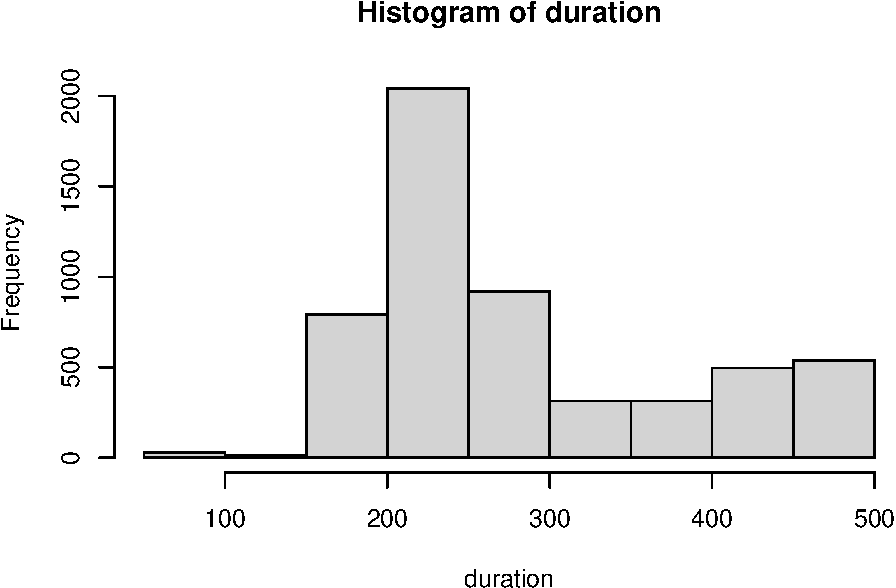
\includegraphics{code4stem_files/figure-latex/make histogram-1.pdf}

\begin{verbatim}
## $breaks
##  [1]  50 100 150 200 250 300 350 400 450 500
## 
## $counts
## [1]   28   15  792 2042  920  314  314  497  538
## 
## $density
## [1] 1.025641e-04 5.494505e-05 2.901099e-03 7.479853e-03 3.369963e-03
## [6] 1.150183e-03 1.150183e-03 1.820513e-03 1.970696e-03
## 
## $mids
## [1]  75 125 175 225 275 325 375 425 475
## 
## $xname
## [1] "duration"
## 
## $equidist
## [1] TRUE
## 
## attr(,"class")
## [1] "histogram"
\end{verbatim}

Computations by groups
Compute the mean duration for every start\_station:

\begin{Shaded}
\begin{Highlighting}[]
\NormalTok{mean_start_stn <-}\StringTok{ }\NormalTok{batrips[, .(}\DataTypeTok{mean_duration =} \KeywordTok{mean}\NormalTok{(duration)), by =}\StringTok{ }\NormalTok{start_station]}
\NormalTok{mean_start_stn }\OperatorTok
\StringTok{  }\KeywordTok{head}\NormalTok{(}\DecValTok{2}\NormalTok{)}
\end{Highlighting}
\end{Shaded}

\begin{verbatim}
##              start_station mean_duration
## 1: San Francisco City Hall      1893.936
## 2:  Embarcadero at Sansome      1418.182
\end{verbatim}

Compute the mean duration for every start and end station:

\begin{Shaded}
\begin{Highlighting}[]
\NormalTok{mean_station <-}\StringTok{ }\NormalTok{batrips[, .(}\DataTypeTok{mean_duration =} \KeywordTok{mean}\NormalTok{(duration)), by =}\StringTok{ }\NormalTok{.(start_station, end_station)]}
\NormalTok{mean_station }\OperatorTok
\StringTok{  }\KeywordTok{head}\NormalTok{(}\DecValTok{2}\NormalTok{)}
\end{Highlighting}
\end{Shaded}

\begin{verbatim}
##              start_station     end_station mean_duration
## 1: San Francisco City Hall Townsend at 7th      678.6364
## 2:  Embarcadero at Sansome Beale at Market      651.2367
\end{verbatim}

Compute the mean duration grouped by start\_station and month:

\begin{Shaded}
\begin{Highlighting}[]
\NormalTok{mean_start_station <-}\StringTok{ }\NormalTok{batrips[, .(}\DataTypeTok{mean_duration =} \KeywordTok{mean}\NormalTok{(duration)), by =}\StringTok{ }\NormalTok{.(start_station, }\KeywordTok{month}\NormalTok{(start_date))]}
\NormalTok{mean_start_station }\OperatorTok
\StringTok{  }\KeywordTok{head}\NormalTok{(}\DecValTok{2}\NormalTok{)}
\end{Highlighting}
\end{Shaded}

\begin{verbatim}
##              start_station month mean_duration
## 1: San Francisco City Hall     1     1548.2591
## 2:  Embarcadero at Sansome     1      952.1756
\end{verbatim}

Compute mean of duration and total trips grouped by start and end stations:

\begin{Shaded}
\begin{Highlighting}[]
\NormalTok{aggregate_mean_trips <-}\StringTok{ }\NormalTok{batrips[, .(}\DataTypeTok{mean_duration =} \KeywordTok{mean}\NormalTok{(duration), }
                                    \DataTypeTok{total_trips =}\NormalTok{ .N), }
\NormalTok{                                by =}\StringTok{ }\NormalTok{.(start_station, end_station)]}
\NormalTok{aggregate_mean_trips }\OperatorTok
\StringTok{  }\KeywordTok{head}\NormalTok{(}\DecValTok{2}\NormalTok{)}
\end{Highlighting}
\end{Shaded}

\begin{verbatim}
##              start_station     end_station mean_duration total_trips
## 1: San Francisco City Hall Townsend at 7th      678.6364         121
## 2:  Embarcadero at Sansome Beale at Market      651.2367         545
\end{verbatim}

Compute min and max duration grouped by start station, end station, and month:

\begin{Shaded}
\begin{Highlighting}[]
\NormalTok{aggregate_min_max <-}\StringTok{ }\NormalTok{batrips[, .(}\DataTypeTok{min_duration =} \KeywordTok{min}\NormalTok{(duration), }
                                 \DataTypeTok{max_duration =} \KeywordTok{max}\NormalTok{(duration)), }
\NormalTok{                             by =}\StringTok{ }\NormalTok{.(start_station, end_station, }
                                    \KeywordTok{month}\NormalTok{(start_date))]}
\NormalTok{aggregate_min_max }\OperatorTok
\StringTok{  }\KeywordTok{head}\NormalTok{(}\DecValTok{2}\NormalTok{)}
\end{Highlighting}
\end{Shaded}

\begin{verbatim}
##              start_station     end_station month min_duration max_duration
## 1: San Francisco City Hall Townsend at 7th     1          370          661
## 2:  Embarcadero at Sansome Beale at Market     1          345         1674
\end{verbatim}

Chaining data.table expressions:
Compute the total trips grouped by start\_station and end\_station

\begin{Shaded}
\begin{Highlighting}[]
\NormalTok{trips_dec <-}\StringTok{ }\NormalTok{batrips[, .N, by =}\StringTok{ }\NormalTok{.(start_station, }
\NormalTok{                                  end_station)]}
\NormalTok{trips_dec }\OperatorTok
\StringTok{  }\KeywordTok{head}\NormalTok{(}\DecValTok{2}\NormalTok{)}
\end{Highlighting}
\end{Shaded}

\begin{verbatim}
##              start_station     end_station   N
## 1: San Francisco City Hall Townsend at 7th 121
## 2:  Embarcadero at Sansome Beale at Market 545
\end{verbatim}

Arrange the total trips grouped by start\_station and end\_station in decreasing order:

\begin{Shaded}
\begin{Highlighting}[]
\NormalTok{trips_dec <-}\StringTok{ }\NormalTok{batrips[, .N, by =}\StringTok{ }\NormalTok{.(start_station, }
\NormalTok{                                  end_station)][}\KeywordTok{order}\NormalTok{(}\OperatorTok{-}\NormalTok{N)]}
\NormalTok{trips_dec }\OperatorTok
\StringTok{  }\KeywordTok{head}\NormalTok{(}\DecValTok{2}\NormalTok{)}
\end{Highlighting}
\end{Shaded}

\begin{verbatim}
##                              start_station
## 1:                         Townsend at 7th
## 2: San Francisco Caltrain 2 (330 Townsend)
##                                 end_station    N
## 1: San Francisco Caltrain (Townsend at 4th) 3158
## 2:                          Townsend at 7th 2937
\end{verbatim}

Top five most popular destinations:

\begin{Shaded}
\begin{Highlighting}[]
\NormalTok{top_}\DecValTok{5}\NormalTok{ <-}\StringTok{ }\NormalTok{batrips[, .N, by =}\StringTok{ }\NormalTok{end_station][}\KeywordTok{order}\NormalTok{(}\OperatorTok{-}\NormalTok{N)][}\DecValTok{1}\OperatorTok{:}\DecValTok{5}\NormalTok{]}
\NormalTok{top_}\DecValTok{5}
\end{Highlighting}
\end{Shaded}

\begin{verbatim}
##                                 end_station     N
## 1: San Francisco Caltrain (Townsend at 4th) 33213
## 2:     Harry Bridges Plaza (Ferry Building) 15692
## 3:  San Francisco Caltrain 2 (330 Townsend) 15333
## 4:                        Market at Sansome 14816
## 5:                          2nd at Townsend 14064
\end{verbatim}

Compute most popular end station for every start station:

\begin{Shaded}
\begin{Highlighting}[]
\NormalTok{popular_end_station <-}\StringTok{ }\NormalTok{trips_dec[, .(}\DataTypeTok{end_station =}\NormalTok{ end_station[}\DecValTok{1}\NormalTok{]), }
\NormalTok{                                 by =}\StringTok{ }\NormalTok{start_station]}
\NormalTok{popular_end_station }\OperatorTok
\StringTok{  }\KeywordTok{head}\NormalTok{(}\DecValTok{2}\NormalTok{)}
\end{Highlighting}
\end{Shaded}

\begin{verbatim}
##                              start_station
## 1:                         Townsend at 7th
## 2: San Francisco Caltrain 2 (330 Townsend)
##                                 end_station
## 1: San Francisco Caltrain (Townsend at 4th)
## 2:                          Townsend at 7th
\end{verbatim}

Find the first and last ride for each start\_station:

\begin{Shaded}
\begin{Highlighting}[]
\NormalTok{first_last <-}\StringTok{ }\NormalTok{batrips[}\KeywordTok{order}\NormalTok{(start_date), }
\NormalTok{                      .(}\DataTypeTok{start_date =}\NormalTok{ start_date[}\KeywordTok{c}\NormalTok{(}\DecValTok{1}\NormalTok{, .N)]), }
\NormalTok{                      by =}\StringTok{ }\NormalTok{start_station]}
\NormalTok{first_last}
\end{Highlighting}
\end{Shaded}

\begin{verbatim}
##                        start_station          start_date
##   1:         San Francisco City Hall 2014-01-01 00:14:00
##   2:         San Francisco City Hall 2014-12-31 22:06:00
##   3:          Embarcadero at Sansome 2014-01-01 00:17:00
##   4:          Embarcadero at Sansome 2014-12-31 22:08:00
##   5:               Steuart at Market 2014-01-01 00:23:00
##  ---                                                    
## 144: Santa Clara County Civic Center 2014-12-31 15:32:00
## 145:                     Ryland Park 2014-04-10 09:10:00
## 146:                     Ryland Park 2014-12-31 07:56:00
## 147:        Stanford in Redwood City 2014-09-03 19:41:00
## 148:        Stanford in Redwood City 2014-12-22 16:56:00
\end{verbatim}

Using .SD (I)

\begin{Shaded}
\begin{Highlighting}[]
\NormalTok{relevant_cols <-}\StringTok{ }\KeywordTok{c}\NormalTok{(}\StringTok{"start_station"}\NormalTok{, }\StringTok{"end_station"}\NormalTok{, }
                   \StringTok{"start_date"}\NormalTok{, }\StringTok{"end_date"}\NormalTok{, }\StringTok{"duration"}\NormalTok{)}
\end{Highlighting}
\end{Shaded}

Find the row corresponding to the shortest trip per month:

\begin{Shaded}
\begin{Highlighting}[]
\NormalTok{shortest <-}\StringTok{ }\NormalTok{batrips[, .SD[}\KeywordTok{which.min}\NormalTok{(duration)], }
\NormalTok{                    by =}\StringTok{ }\KeywordTok{month}\NormalTok{(start_date), }
\NormalTok{                    .SDcols =}\StringTok{ }\NormalTok{relevant_cols]}
\NormalTok{shortest }\OperatorTok
\StringTok{  }\KeywordTok{head}\NormalTok{(}\DecValTok{2}\NormalTok{)}
\end{Highlighting}
\end{Shaded}

\begin{verbatim}
##    month                            start_station
## 1:     1                          2nd at Townsend
## 2:     2 San Francisco Caltrain (Townsend at 4th)
##                                 end_station          start_date
## 1:                          2nd at Townsend 2014-01-21 13:01:00
## 2: San Francisco Caltrain (Townsend at 4th) 2014-02-08 14:28:00
##               end_date duration
## 1: 2014-01-21 13:02:00       60
## 2: 2014-02-08 14:29:00       61
\end{verbatim}

Using .SD (II)
Find the total number of unique start stations and zip codes per month:

\begin{Shaded}
\begin{Highlighting}[]
\NormalTok{unique_station_month <-}\StringTok{ }\NormalTok{batrips[, }\KeywordTok{lapply}\NormalTok{(.SD, uniqueN), }
\NormalTok{                                by =}\StringTok{ }\KeywordTok{month}\NormalTok{(start_date), }
\NormalTok{                                .SDcols =}\StringTok{ }\KeywordTok{c}\NormalTok{(}\StringTok{"start_station"}\NormalTok{, }\StringTok{"zip_code"}\NormalTok{)]}
\NormalTok{unique_station_month }\OperatorTok
\StringTok{  }\KeywordTok{head}\NormalTok{(}\DecValTok{2}\NormalTok{)}
\end{Highlighting}
\end{Shaded}

\begin{verbatim}
##    month start_station zip_code
## 1:     1            68      710
## 2:     2            69      591
\end{verbatim}

Adding and updating columns by reference
Add a new column, duration\_hour:

\begin{Shaded}
\begin{Highlighting}[]
\NormalTok{batrips[, duration_hour }\OperatorTok{:}\ErrorTok{=}\StringTok{ }\NormalTok{duration }\OperatorTok{/}\StringTok{ }\DecValTok{3600}\NormalTok{]}
\end{Highlighting}
\end{Shaded}

Fix/edit spelling in the second row of start\_station:

\begin{Shaded}
\begin{Highlighting}[]
\NormalTok{batrips[}\DecValTok{2}\NormalTok{, start_station }\OperatorTok{:}\ErrorTok{=}\StringTok{ "San Francisco City Hall 2"}\NormalTok{]}
\end{Highlighting}
\end{Shaded}

Replace negative duration values with NA:

\begin{Shaded}
\begin{Highlighting}[]
\NormalTok{batrips[duration }\OperatorTok{<}\StringTok{ }\DecValTok{0}\NormalTok{, duration }\OperatorTok{:}\ErrorTok{=}\StringTok{ }\OtherTok{NA}\NormalTok{]}
\end{Highlighting}
\end{Shaded}

Add a new column equal to total trips for every start station:

\begin{Shaded}
\begin{Highlighting}[]
\NormalTok{batrips[, trips_N }\OperatorTok{:}\ErrorTok{=}\StringTok{ }\NormalTok{.N, by =}\StringTok{ }\NormalTok{start_station]}
\end{Highlighting}
\end{Shaded}

Add new column for every start\_station and end\_station:

\begin{Shaded}
\begin{Highlighting}[]
\NormalTok{batrips[, duration_mean }\OperatorTok{:}\ErrorTok{=}\StringTok{ }\KeywordTok{mean}\NormalTok{(duration), by =}\StringTok{ }\NormalTok{.(start_station, end_station)]}
\end{Highlighting}
\end{Shaded}

Calculate the mean duration for each month:

\begin{Shaded}
\begin{Highlighting}[]
\NormalTok{batrips[, mean_dur }\OperatorTok{:}\ErrorTok{=}\StringTok{ }\KeywordTok{mean}\NormalTok{(duration, }\DataTypeTok{na.rm =} \OtherTok{TRUE}\NormalTok{), }
\NormalTok{            by =}\StringTok{ }\KeywordTok{month}\NormalTok{(start_date)]}
\end{Highlighting}
\end{Shaded}

Replace NA values in duration with the mean value of duration for that month:

\begin{Shaded}
\begin{Highlighting}[]
\NormalTok{batrips[, mean_dur }\OperatorTok{:}\ErrorTok{=}\StringTok{ }\KeywordTok{mean}\NormalTok{(duration, }\DataTypeTok{na.rm =} \OtherTok{TRUE}\NormalTok{), }
\NormalTok{            by =}\StringTok{ }\KeywordTok{month}\NormalTok{(start_date)][}\KeywordTok{is.na}\NormalTok{(duration), }
\NormalTok{                                    duration }\OperatorTok{:}\ErrorTok{=}\StringTok{ }\NormalTok{mean_dur]}
\end{Highlighting}
\end{Shaded}

Delete the mean\_dur column by reference:

\begin{Shaded}
\begin{Highlighting}[]
\NormalTok{batrips[, mean_dur }\OperatorTok{:}\ErrorTok{=}\StringTok{ }\KeywordTok{mean}\NormalTok{(duration, }\DataTypeTok{na.rm =} \OtherTok{TRUE}\NormalTok{), }
\NormalTok{            by =}\StringTok{ }\KeywordTok{month}\NormalTok{(start_date)][}\KeywordTok{is.na}\NormalTok{(duration), }
\NormalTok{                                    duration }\OperatorTok{:}\ErrorTok{=}\StringTok{ }\NormalTok{mean_dur][, mean_dur }\OperatorTok{:}\ErrorTok{=}\StringTok{ }\OtherTok{NULL}\NormalTok{]}
\end{Highlighting}
\end{Shaded}

Add columns using the LHS := RHS form
LHS := RHS form. In the LHS, you specify column names as a character vector and in the RHS, you specify values/expressions to be added inside list() (or the alias, .()):

\begin{Shaded}
\begin{Highlighting}[]
\NormalTok{batrips[, }\KeywordTok{c}\NormalTok{(}\StringTok{"mean_duration"}\NormalTok{, }
            \StringTok{"median_duration"}\NormalTok{) }\OperatorTok{:}\ErrorTok{=}\StringTok{ }\NormalTok{.(}\KeywordTok{mean}\NormalTok{(duration), }\KeywordTok{median}\NormalTok{(duration)), }
\NormalTok{        by =}\StringTok{ }\NormalTok{start_station]}
\end{Highlighting}
\end{Shaded}

Add columns using the functional form:

\begin{Shaded}
\begin{Highlighting}[]
\NormalTok{batrips[, }\StringTok{`}\DataTypeTok{:=}\StringTok{`}\NormalTok{(}\DataTypeTok{mean_duration =} \KeywordTok{mean}\NormalTok{(duration), }
               \DataTypeTok{median_duration =} \KeywordTok{median}\NormalTok{(duration)), }
\NormalTok{        by =}\StringTok{ }\NormalTok{start_station]}
\end{Highlighting}
\end{Shaded}

Add the mean\_duration column:

\begin{Shaded}
\begin{Highlighting}[]
\NormalTok{batrips[duration }\OperatorTok{>}\StringTok{ }\DecValTok{600}\NormalTok{, mean_duration }\OperatorTok{:}\ErrorTok{=}\StringTok{ }\KeywordTok{mean}\NormalTok{(duration), }
\NormalTok{        by =}\StringTok{ }\NormalTok{.(start_station, end_station)]}
\end{Highlighting}
\end{Shaded}

Use read.csv() to import batrips
Fread is much faster!

\begin{itemize}
\tightlist
\item
  system.time(read.csv(``batrips.csv''))
\item
  system.time(fread(``batrips.csv''))
\end{itemize}

Import using read.csv():

\begin{Shaded}
\begin{Highlighting}[]
\NormalTok{csv_file <-}\StringTok{ }\KeywordTok{read.csv}\NormalTok{(}\StringTok{"data/sample.csv"}\NormalTok{, }\DataTypeTok{fill =} \OtherTok{NA}\NormalTok{, }\DataTypeTok{quote =} \StringTok{""}\NormalTok{, }
                     \DataTypeTok{stringsAsFactors =} \OtherTok{FALSE}\NormalTok{, }\DataTypeTok{strip.white =} \OtherTok{TRUE}\NormalTok{, }
                     \DataTypeTok{header =} \OtherTok{TRUE}\NormalTok{)}
\NormalTok{csv_file }\OperatorTok
\StringTok{  }\KeywordTok{head}\NormalTok{(}\DecValTok{2}\NormalTok{)}
\end{Highlighting}
\end{Shaded}

\begin{verbatim}
##   YEAR    GEO Age_group  Sex                                     Element
## 1 1980 Canada         0 Both           Number of survivors at age x (lx)
## 2 1980 Canada         0 Both Number of deaths between age x and x+1 (dx)
##   AVG_VALUE
## 1    100000
## 2       976
\end{verbatim}

Import using fread():

\begin{Shaded}
\begin{Highlighting}[]
\NormalTok{csv_file <-}\StringTok{ }\KeywordTok{fread}\NormalTok{(}\StringTok{"data/sample.csv"}\NormalTok{)}
\NormalTok{csv_file }\OperatorTok
\StringTok{  }\KeywordTok{head}\NormalTok{(}\DecValTok{2}\NormalTok{)}
\end{Highlighting}
\end{Shaded}

\begin{verbatim}
##    YEAR    GEO Age_group  Sex                                     Element
## 1: 1980 Canada         0 Both           Number of survivors at age x (lx)
## 2: 1980 Canada         0 Both Number of deaths between age x and x+1 (dx)
##    AVG_VALUE
## 1:    100000
## 2:       976
\end{verbatim}

Check the class of Sex column:

\begin{Shaded}
\begin{Highlighting}[]
\KeywordTok{class}\NormalTok{(csv_file}\OperatorTok{$}\NormalTok{Sex)}
\end{Highlighting}
\end{Shaded}

\begin{verbatim}
## [1] "character"
\end{verbatim}

Import using read.csv with defaults:

\begin{Shaded}
\begin{Highlighting}[]
\KeywordTok{str}\NormalTok{(csv_file)}
\end{Highlighting}
\end{Shaded}

\begin{verbatim}
## Classes 'data.table' and 'data.frame':	1048575 obs. of  6 variables:
##  $ YEAR     : int  1980 1980 1980 1980 1980 1980 1980 1980 1980 1980 ...
##  $ GEO      : chr  "Canada" "Canada" "Canada" "Canada" ...
##  $ Age_group: int  0 0 0 0 0 0 0 0 0 0 ...
##  $ Sex      : chr  "Both" "Both" "Both" "Both" ...
##  $ Element  : chr  "Number of survivors at age x (lx)" "Number of deaths between age x and x+1 (dx)" "Death probability between age x and x+1 (qx)" "Margin of error of the death probability (m.e.(qx))" ...
##  $ AVG_VALUE: num  1.00e+05 9.76e+02 9.76e-03 1.80e-04 9.90e-01 ...
##  - attr(*, ".internal.selfref")=<externalptr>
\end{verbatim}

Select ``id'' and ``val'' columns:

\begin{Shaded}
\begin{Highlighting}[]
\NormalTok{select_columns <-}\StringTok{ }\KeywordTok{fread}\NormalTok{(}\StringTok{"data/sample.csv"}\NormalTok{, }\DataTypeTok{select =} \KeywordTok{c}\NormalTok{(}\StringTok{"GEO"}\NormalTok{, }\StringTok{"Sex"}\NormalTok{))}
\NormalTok{select_columns }\OperatorTok
\StringTok{  }\KeywordTok{head}\NormalTok{(}\DecValTok{2}\NormalTok{)}
\end{Highlighting}
\end{Shaded}

\begin{verbatim}
##       GEO  Sex
## 1: Canada Both
## 2: Canada Both
\end{verbatim}

Drop the ``val'' column:

\begin{Shaded}
\begin{Highlighting}[]
\NormalTok{drop_column <-}\StringTok{ }\KeywordTok{fread}\NormalTok{(}\StringTok{"data/sample.csv"}\NormalTok{, }\DataTypeTok{drop =} \StringTok{"Sex"}\NormalTok{)}
\NormalTok{drop_column }\OperatorTok
\StringTok{  }\KeywordTok{head}\NormalTok{(}\DecValTok{2}\NormalTok{)}
\end{Highlighting}
\end{Shaded}

\begin{verbatim}
##    YEAR    GEO Age_group                                     Element AVG_VALUE
## 1: 1980 Canada         0           Number of survivors at age x (lx)    100000
## 2: 1980 Canada         0 Number of deaths between age x and x+1 (dx)       976
\end{verbatim}

Import the file while avoiding the warning:

\begin{Shaded}
\begin{Highlighting}[]
\NormalTok{only_data <-}\StringTok{ }\KeywordTok{fread}\NormalTok{(}\StringTok{"data/sample.csv"}\NormalTok{, }\DataTypeTok{nrows =} \DecValTok{3}\NormalTok{)}
\NormalTok{only_data}
\end{Highlighting}
\end{Shaded}

\begin{verbatim}
##    YEAR    GEO Age_group  Sex                                      Element
## 1: 1980 Canada         0 Both            Number of survivors at age x (lx)
## 2: 1980 Canada         0 Both  Number of deaths between age x and x+1 (dx)
## 3: 1980 Canada         0 Both Death probability between age x and x+1 (qx)
##    AVG_VALUE
## 1:  1.00e+05
## 2:  9.76e+02
## 3:  9.76e-03
\end{verbatim}

Import only the metadata:

\begin{Shaded}
\begin{Highlighting}[]
\NormalTok{only_metadata <-}\StringTok{ }\KeywordTok{fread}\NormalTok{(}\StringTok{"data/sample.csv"}\NormalTok{, }\DataTypeTok{skip =} \DecValTok{7}\NormalTok{)}
\NormalTok{only_metadata }\OperatorTok
\StringTok{  }\KeywordTok{head}\NormalTok{(}\DecValTok{2}\NormalTok{)}
\end{Highlighting}
\end{Shaded}

\begin{verbatim}
##      V1     V2 V3   V4                                                      V5
## 1: 1980 Canada  0 Both Cumulative number of life years lived beyond age x (Tx)
## 2: 1980 Canada  0 Both                Life expectancy (in years) at age x (ex)
##           V6
## 1: 7543058.0
## 2:      75.4
\end{verbatim}

Import using read.csv:

\begin{Shaded}
\begin{Highlighting}[]
\NormalTok{base_r <-}\StringTok{ }\KeywordTok{read.csv}\NormalTok{(}\StringTok{"data/sample.csv"}\NormalTok{, }
                   \DataTypeTok{colClasses =} \KeywordTok{c}\NormalTok{(}\KeywordTok{rep}\NormalTok{(}\StringTok{"factor"}\NormalTok{, }\DecValTok{4}\NormalTok{), }
                                  \StringTok{"character"}\NormalTok{, }
                                  \StringTok{"numeric"}\NormalTok{))}
\KeywordTok{str}\NormalTok{(base_r)}
\end{Highlighting}
\end{Shaded}

\begin{verbatim}
## 'data.frame':	1048575 obs. of  6 variables:
##  $ YEAR     : Factor w/ 35 levels "1980","1981",..: 1 1 1 1 1 1 1 1 1 1 ...
##  $ GEO      : Factor w/ 10 levels "Alberta","British Columbia",..: 3 3 3 3 3 3 3 3 3 3 ...
##  $ Age_group: Factor w/ 111 levels "0","1","10","100",..: 1 1 1 1 1 1 1 1 1 1 ...
##  $ Sex      : Factor w/ 3 levels "Both","F","M": 1 1 1 1 1 1 1 1 1 3 ...
##  $ Element  : chr  "Number of survivors at age x (lx)" "Number of deaths between age x and x+1 (dx)" "Death probability between age x and x+1 (qx)" "Margin of error of the death probability (m.e.(qx))" ...
##  $ AVG_VALUE: num  1.00e+05 9.76e+02 9.76e-03 1.80e-04 9.90e-01 ...
\end{verbatim}

Import using fread:

\begin{Shaded}
\begin{Highlighting}[]
\NormalTok{import_fread <-}\StringTok{ }\KeywordTok{fread}\NormalTok{(}\StringTok{"data/sample.csv"}\NormalTok{, }
                      \DataTypeTok{colClasses =} \KeywordTok{list}\NormalTok{(}\DataTypeTok{factor =} \DecValTok{1}\OperatorTok{:}\DecValTok{4}\NormalTok{, }\DataTypeTok{numeric =} \DecValTok{7}\OperatorTok{:}\DecValTok{10}\NormalTok{))}
\end{Highlighting}
\end{Shaded}

\begin{verbatim}
## Warning in fread("data/sample.csv", colClasses = list(factor = 1:4, numeric =
## 7:10)): Column number 7 (colClasses[[2]][1]) is out of range [1,ncol=6]
\end{verbatim}

\begin{verbatim}
## Warning in fread("data/sample.csv", colClasses = list(factor = 1:4, numeric =
## 7:10)): Column number 8 (colClasses[[2]][2]) is out of range [1,ncol=6]
\end{verbatim}

\begin{verbatim}
## Warning in fread("data/sample.csv", colClasses = list(factor = 1:4, numeric =
## 7:10)): Column number 9 (colClasses[[2]][3]) is out of range [1,ncol=6]
\end{verbatim}

\begin{verbatim}
## Warning in fread("data/sample.csv", colClasses = list(factor = 1:4, numeric =
## 7:10)): Column number 10 (colClasses[[2]][4]) is out of range [1,ncol=6]
\end{verbatim}

\begin{Shaded}
\begin{Highlighting}[]
\KeywordTok{str}\NormalTok{(import_fread)}
\end{Highlighting}
\end{Shaded}

\begin{verbatim}
## Classes 'data.table' and 'data.frame':	1048575 obs. of  6 variables:
##  $ YEAR     : Factor w/ 35 levels "1980","1981",..: 1 1 1 1 1 1 1 1 1 1 ...
##  $ GEO      : Factor w/ 10 levels "Alberta","British Columbia",..: 3 3 3 3 3 3 3 3 3 3 ...
##  $ Age_group: Factor w/ 111 levels "0","1","10","100",..: 1 1 1 1 1 1 1 1 1 1 ...
##  $ Sex      : Factor w/ 3 levels "Both","F","M": 1 1 1 1 1 1 1 1 1 3 ...
##  $ Element  : chr  "Number of survivors at age x (lx)" "Number of deaths between age x and x+1 (dx)" "Death probability between age x and x+1 (qx)" "Margin of error of the death probability (m.e.(qx))" ...
##  $ AVG_VALUE: num  1.00e+05 9.76e+02 9.76e-03 1.80e-04 9.90e-01 ...
##  - attr(*, ".internal.selfref")=<externalptr>
\end{verbatim}

Import the file correctly, use the fill argument to ensure all rows are imported correctly:

\begin{Shaded}
\begin{Highlighting}[]
\NormalTok{correct <-}\StringTok{ }\KeywordTok{fread}\NormalTok{(}\StringTok{"data/sample.csv"}\NormalTok{, }\DataTypeTok{fill =} \OtherTok{TRUE}\NormalTok{)}
\NormalTok{correct }\OperatorTok
\StringTok{  }\KeywordTok{head}\NormalTok{(}\DecValTok{2}\NormalTok{)}
\end{Highlighting}
\end{Shaded}

\begin{verbatim}
##    YEAR    GEO Age_group  Sex                                     Element
## 1: 1980 Canada         0 Both           Number of survivors at age x (lx)
## 2: 1980 Canada         0 Both Number of deaths between age x and x+1 (dx)
##    AVG_VALUE
## 1:    100000
## 2:       976
\end{verbatim}

Import the file using na.strings
The missing values are encoded as ``\#\#''. Note that fread() handles an empty field ,, by default as NA

\begin{Shaded}
\begin{Highlighting}[]
\NormalTok{missing_values <-}\StringTok{ }\KeywordTok{fread}\NormalTok{(}\StringTok{"data/sample.csv"}\NormalTok{, }\DataTypeTok{na.strings =} \StringTok{"##"}\NormalTok{) }
\NormalTok{missing_values }\OperatorTok
\StringTok{  }\KeywordTok{head}\NormalTok{(}\DecValTok{2}\NormalTok{)}
\end{Highlighting}
\end{Shaded}

\begin{verbatim}
##    YEAR    GEO Age_group  Sex                                     Element
## 1: 1980 Canada         0 Both           Number of survivors at age x (lx)
## 2: 1980 Canada         0 Both Number of deaths between age x and x+1 (dx)
##    AVG_VALUE
## 1:  1.00E+05
## 2:       976
\end{verbatim}

Write dt to fwrite.txt:
- fwrite(dt, ``fwrite.txt'')

Import the file using readLines():

\begin{Shaded}
\begin{Highlighting}[]
\KeywordTok{readLines}\NormalTok{(}\StringTok{"data/sample.csv"}\NormalTok{) }\OperatorTok
\StringTok{  }\KeywordTok{head}\NormalTok{(}\DecValTok{2}\NormalTok{)}
\end{Highlighting}
\end{Shaded}

\begin{verbatim}
## Warning in readLines("data/sample.csv"): incomplete final line found on 'data/
## sample.csv'
\end{verbatim}

\begin{verbatim}
## [1] "YEAR,GEO,Age_group,Sex,Element,AVG_VALUE"                     
## [2] "1980,Canada,0,Both,Number of survivors at age x (lx),1.00E+05"
\end{verbatim}

Write batrips\_dates to file using ``ISO'' format:
- fwrite(batrips\_dates, ``iso.txt'', dateTimeAs = ``ISO'')

Write batrips\_dates to file using ``squash'' format:
- fwrite(batrips\_dates, ``squash.txt'', dateTimeAs = ``squash'')

\hypertarget{tests-for-experiments}{%
\chapter{Tests for experiments}\label{tests-for-experiments}}

Prior to performing experiments, we need to set the dependent variables (outcome), and independent variables (explanatory variables).

Other experimental components to consider include randomization, replication, blocking

\begin{Shaded}
\begin{Highlighting}[]
\CommentTok{# load dependencies}
\KeywordTok{library}\NormalTok{(ggplot2) }
\KeywordTok{library}\NormalTok{(broom)}
\KeywordTok{library}\NormalTok{(tidyverse)}
\KeywordTok{library}\NormalTok{(pwr)}
\KeywordTok{library}\NormalTok{(haven)}
\KeywordTok{library}\NormalTok{(simputation)}
\KeywordTok{library}\NormalTok{(sampling)}
\KeywordTok{library}\NormalTok{(agricolae)}
\KeywordTok{library}\NormalTok{(naniar)}
\KeywordTok{library}\NormalTok{(DescTools)}
\KeywordTok{library}\NormalTok{(mice)}
\end{Highlighting}
\end{Shaded}

load data: Dataset is on the Effect of Vitamin C on Tooth Growth in Guinea Pigs:

\begin{Shaded}
\begin{Highlighting}[]
\KeywordTok{data}\NormalTok{(ToothGrowth) }

\NormalTok{ToothGrowth }\OperatorTok
\StringTok{  }\KeywordTok{head}\NormalTok{(}\DecValTok{2}\NormalTok{)}
\end{Highlighting}
\end{Shaded}

\begin{verbatim}
##    len supp dose
## 1  4.2   VC  0.5
## 2 11.5   VC  0.5
\end{verbatim}

Perform a two-sided t-test:

\begin{Shaded}
\begin{Highlighting}[]
\KeywordTok{t.test}\NormalTok{(}\DataTypeTok{x =}\NormalTok{ ToothGrowth}\OperatorTok{$}\NormalTok{len, }\DataTypeTok{alternative =} \StringTok{"two.sided"}\NormalTok{, }\DataTypeTok{mu =} \DecValTok{18}\NormalTok{)}
\end{Highlighting}
\end{Shaded}

\begin{verbatim}
## 
## 	One Sample t-test
## 
## data:  ToothGrowth$len
## t = 0.82361, df = 59, p-value = 0.4135
## alternative hypothesis: true mean is not equal to 18
## 95 percent confidence interval:
##  16.83731 20.78936
## sample estimates:
## mean of x 
##  18.81333
\end{verbatim}

Perform a t-test

\begin{Shaded}
\begin{Highlighting}[]
\NormalTok{ToothGrowth_ttest <-}\StringTok{ }\KeywordTok{t.test}\NormalTok{(len }\OperatorTok{~}\StringTok{ }\NormalTok{supp, }\DataTypeTok{data =}\NormalTok{ ToothGrowth)}
\NormalTok{ToothGrowth_ttest}
\end{Highlighting}
\end{Shaded}

\begin{verbatim}
## 
## 	Welch Two Sample t-test
## 
## data:  len by supp
## t = 1.9153, df = 55.309, p-value = 0.06063
## alternative hypothesis: true difference in means is not equal to 0
## 95 percent confidence interval:
##  -0.1710156  7.5710156
## sample estimates:
## mean in group OJ mean in group VC 
##         20.66333         16.96333
\end{verbatim}

Tidy ToothGrowth\_ttest:

\begin{Shaded}
\begin{Highlighting}[]
\KeywordTok{tidy}\NormalTok{(ToothGrowth_ttest)}
\end{Highlighting}
\end{Shaded}

\begin{verbatim}
## # A tibble: 1 x 10
##   estimate estimate1 estimate2 statistic p.value parameter conf.low conf.high
##      <dbl>     <dbl>     <dbl>     <dbl>   <dbl>     <dbl>    <dbl>     <dbl>
## 1     3.70      20.7      17.0      1.92  0.0606      55.3   -0.171      7.57
## # ... with 2 more variables: method <chr>, alternative <chr>
\end{verbatim}

Replication:
Count number of observations for each combination of supp and dose

\begin{Shaded}
\begin{Highlighting}[]
\NormalTok{ToothGrowth }\OperatorTok\StringTok{ }
\StringTok{  }\KeywordTok{count}\NormalTok{(supp, dose) }
\end{Highlighting}
\end{Shaded}

\begin{verbatim}
##   supp dose  n
## 1   OJ  0.5 10
## 2   OJ  1.0 10
## 3   OJ  2.0 10
## 4   VC  0.5 10
## 5   VC  1.0 10
## 6   VC  2.0 10
\end{verbatim}

Blocking:
Create a boxplot with geom\_boxplot()
aov() creates a linear regression model by calling lm() and examining results with anova() all in one function call.

\begin{Shaded}
\begin{Highlighting}[]
\KeywordTok{ggplot}\NormalTok{(ToothGrowth, }\KeywordTok{aes}\NormalTok{(}\DataTypeTok{x =}\NormalTok{ dose, }\DataTypeTok{y =}\NormalTok{ len)) }\OperatorTok{+}\StringTok{ }
\StringTok{  }\KeywordTok{geom_boxplot}\NormalTok{()}
\end{Highlighting}
\end{Shaded}

\begin{verbatim}
## Warning: Continuous x aesthetic -- did you forget aes(group=...)?
\end{verbatim}

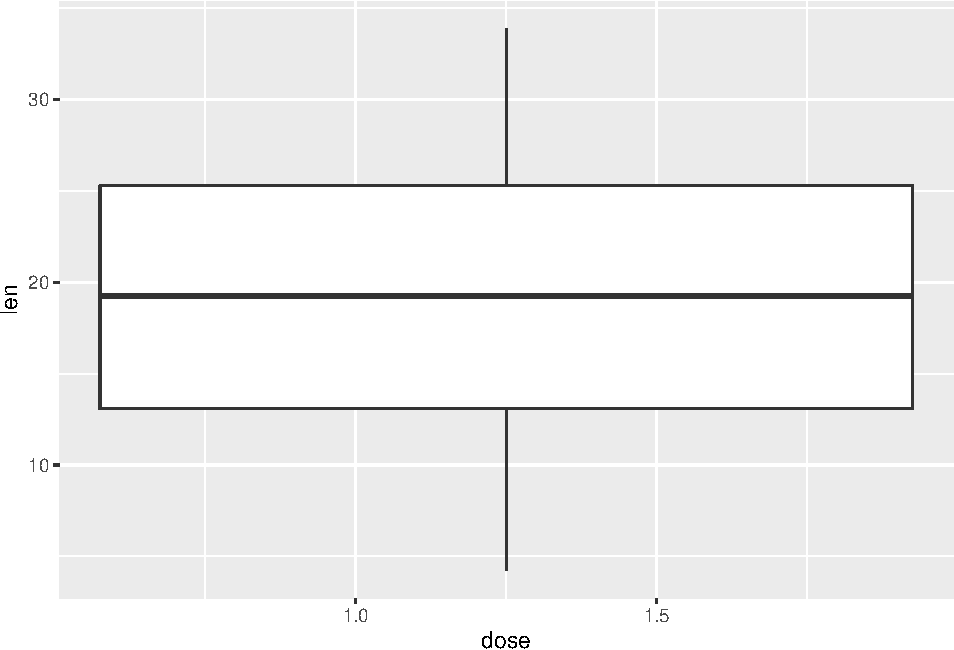
\includegraphics{code4stem_files/figure-latex/Visualize-1.pdf}

Create ToothGrowth\_aov and
Examine ToothGrowth\_aov with summary():

\begin{Shaded}
\begin{Highlighting}[]
\NormalTok{ToothGrowth_aov <-}\StringTok{ }\KeywordTok{aov}\NormalTok{(len }\OperatorTok{~}\StringTok{ }\NormalTok{dose }\OperatorTok{+}\StringTok{ }\NormalTok{supp, }\DataTypeTok{data =}\NormalTok{ ToothGrowth)}
\KeywordTok{summary}\NormalTok{(ToothGrowth_aov)}
\end{Highlighting}
\end{Shaded}

\begin{verbatim}
##             Df Sum Sq Mean Sq F value   Pr(>F)    
## dose         1 2224.3  2224.3  123.99 6.31e-16 ***
## supp         1  205.3   205.3   11.45   0.0013 ** 
## Residuals   57 1022.6    17.9                     
## ---
## Signif. codes:  0 '***' 0.001 '**' 0.01 '*' 0.05 '.' 0.1 ' ' 1
\end{verbatim}

Hypothesis Testing (null and alternative) with \texttt{pwr} package
one sided and two sided tests:
- type ?t.test to find out more

\begin{Shaded}
\begin{Highlighting}[]
\CommentTok{#Less than}
\KeywordTok{t.test}\NormalTok{(}\DataTypeTok{x =}\NormalTok{ ToothGrowth}\OperatorTok{$}\NormalTok{len,}
       \DataTypeTok{alternative =} \StringTok{"less"}\NormalTok{,}
       \DataTypeTok{mu =} \DecValTok{18}\NormalTok{)}
\end{Highlighting}
\end{Shaded}

\begin{verbatim}
## 
## 	One Sample t-test
## 
## data:  ToothGrowth$len
## t = 0.82361, df = 59, p-value = 0.7933
## alternative hypothesis: true mean is less than 18
## 95 percent confidence interval:
##      -Inf 20.46358
## sample estimates:
## mean of x 
##  18.81333
\end{verbatim}

\begin{Shaded}
\begin{Highlighting}[]
\CommentTok{# Greater than}
\KeywordTok{t.test}\NormalTok{(}\DataTypeTok{x =}\NormalTok{ ToothGrowth}\OperatorTok{$}\NormalTok{len,}
       \DataTypeTok{alternative =} \StringTok{"greater"}\NormalTok{,}
       \DataTypeTok{mu =} \DecValTok{18}\NormalTok{)}
\end{Highlighting}
\end{Shaded}

\begin{verbatim}
## 
## 	One Sample t-test
## 
## data:  ToothGrowth$len
## t = 0.82361, df = 59, p-value = 0.2067
## alternative hypothesis: true mean is greater than 18
## 95 percent confidence interval:
##  17.16309      Inf
## sample estimates:
## mean of x 
##  18.81333
\end{verbatim}

It turns out the mean of len is actually very close to 18, so neither of these tests tells us much about the mean of tooth length.
?pwr.t.test()

Calculate sample size:

\begin{Shaded}
\begin{Highlighting}[]
\KeywordTok{pwr.t.test}\NormalTok{(}\DataTypeTok{n =} \OtherTok{NULL}\NormalTok{,}
           \DataTypeTok{d =} \FloatTok{0.25}\NormalTok{,  }\CommentTok{# small effect size of 0.25}
           \DataTypeTok{sig.level =} \FloatTok{0.05}\NormalTok{, }
           \DataTypeTok{type =} \StringTok{"one.sample"}\NormalTok{, }
           \DataTypeTok{alternative =} \StringTok{"greater"}\NormalTok{, }
           \DataTypeTok{power =} \FloatTok{0.8}\NormalTok{)}
\end{Highlighting}
\end{Shaded}

\begin{verbatim}
## 
##      One-sample t test power calculation 
## 
##               n = 100.2877
##               d = 0.25
##       sig.level = 0.05
##           power = 0.8
##     alternative = greater
\end{verbatim}

Calculate power:

\begin{Shaded}
\begin{Highlighting}[]
\KeywordTok{pwr.t.test}\NormalTok{(}\DataTypeTok{n =} \DecValTok{100}\NormalTok{,}
           \DataTypeTok{d =} \FloatTok{0.35}\NormalTok{,}
           \DataTypeTok{sig.level =} \FloatTok{0.1}\NormalTok{,}
           \DataTypeTok{type =} \StringTok{"two.sample"}\NormalTok{,}
           \DataTypeTok{alternative =} \StringTok{"two.sided"}\NormalTok{,}
           \DataTypeTok{power =} \OtherTok{NULL}\NormalTok{)}
\end{Highlighting}
\end{Shaded}

\begin{verbatim}
## 
##      Two-sample t test power calculation 
## 
##               n = 100
##               d = 0.35
##       sig.level = 0.1
##           power = 0.7943532
##     alternative = two.sided
## 
## NOTE: n is number in *each* group
\end{verbatim}

power for multiple groups:

\begin{Shaded}
\begin{Highlighting}[]
\KeywordTok{pwr.anova.test}\NormalTok{(}\DataTypeTok{k =} \DecValTok{3}\NormalTok{,}
               \DataTypeTok{n =} \DecValTok{20}\NormalTok{,}
               \DataTypeTok{f =} \FloatTok{0.2}\NormalTok{, }\CommentTok{#effect size}
               \DataTypeTok{sig.level =} \FloatTok{0.05}\NormalTok{,}
               \DataTypeTok{power =} \OtherTok{NULL}\NormalTok{)}
\end{Highlighting}
\end{Shaded}

\begin{verbatim}
## 
##      Balanced one-way analysis of variance power calculation 
## 
##               k = 3
##               n = 20
##               f = 0.2
##       sig.level = 0.05
##           power = 0.2521043
## 
## NOTE: n is number in each group
\end{verbatim}

Anova tests (for multiple groups) can be done in two ways

Basic Experiments for exploratory data analysis including A/B testing

get data:

\begin{Shaded}
\begin{Highlighting}[]
\KeywordTok{data}\NormalTok{(txhousing)}

\NormalTok{txhousing }\OperatorTok
\StringTok{  }\KeywordTok{head}\NormalTok{(}\DecValTok{2}\NormalTok{)}
\end{Highlighting}
\end{Shaded}

\begin{verbatim}
## # A tibble: 2 x 9
##   city     year month sales  volume median listings inventory  date
##   <chr>   <int> <int> <dbl>   <dbl>  <dbl>    <dbl>     <dbl> <dbl>
## 1 Abilene  2000     1    72 5380000  71400      701       6.3 2000 
## 2 Abilene  2000     2    98 6505000  58700      746       6.6 2000.
\end{verbatim}

remove NAs:

\begin{Shaded}
\begin{Highlighting}[]
\NormalTok{tx_housing <-}\StringTok{ }\KeywordTok{na.omit}\NormalTok{(txhousing)}

\CommentTok{# Examine the variables with glimpse()}
\KeywordTok{glimpse}\NormalTok{(tx_housing)}
\end{Highlighting}
\end{Shaded}

\begin{verbatim}
## Rows: 7,126
## Columns: 9
## $ city      <chr> "Abilene", "Abilene", "Abilene", "Abilene", "Abilene", "A...
## $ year      <int> 2000, 2000, 2000, 2000, 2000, 2000, 2000, 2000, 2000, 200...
## $ month     <int> 1, 2, 3, 4, 5, 6, 7, 8, 9, 10, 11, 12, 1, 2, 3, 4, 5, 6, ...
## $ sales     <dbl> 72, 98, 130, 98, 141, 156, 152, 131, 104, 101, 100, 92, 7...
## $ volume    <dbl> 5380000, 6505000, 9285000, 9730000, 10590000, 13910000, 1...
## $ median    <dbl> 71400, 58700, 58100, 68600, 67300, 66900, 73500, 75000, 6...
## $ listings  <dbl> 701, 746, 784, 785, 794, 780, 742, 765, 771, 764, 721, 65...
## $ inventory <dbl> 6.3, 6.6, 6.8, 6.9, 6.8, 6.6, 6.2, 6.4, 6.5, 6.6, 6.2, 5....
## $ date      <dbl> 2000.000, 2000.083, 2000.167, 2000.250, 2000.333, 2000.41...
\end{verbatim}

Find median and means with summarize():

\begin{Shaded}
\begin{Highlighting}[]
\NormalTok{tx_housing }\OperatorTok\StringTok{ }
\StringTok{  }\KeywordTok{summarize}\NormalTok{(}\KeywordTok{median}\NormalTok{(volume), }\KeywordTok{mean}\NormalTok{(sales), }\KeywordTok{mean}\NormalTok{(inventory))}
\end{Highlighting}
\end{Shaded}

\begin{verbatim}
## # A tibble: 1 x 3
##   `median(volume)` `mean(sales)` `mean(inventory)`
##              <dbl>         <dbl>             <dbl>
## 1        26240116.          603.              7.17
\end{verbatim}

Use ggplot2 to build a bar chart of purpose:

\begin{Shaded}
\begin{Highlighting}[]
\KeywordTok{ggplot}\NormalTok{(}\DataTypeTok{data=}\NormalTok{tx_housing, }\KeywordTok{aes}\NormalTok{(}\DataTypeTok{x =}\NormalTok{ city)) }\OperatorTok{+}\StringTok{ }
\StringTok{  }\KeywordTok{geom_bar}\NormalTok{() }\OperatorTok{+}
\StringTok{  }\KeywordTok{coord_flip}\NormalTok{()}
\end{Highlighting}
\end{Shaded}

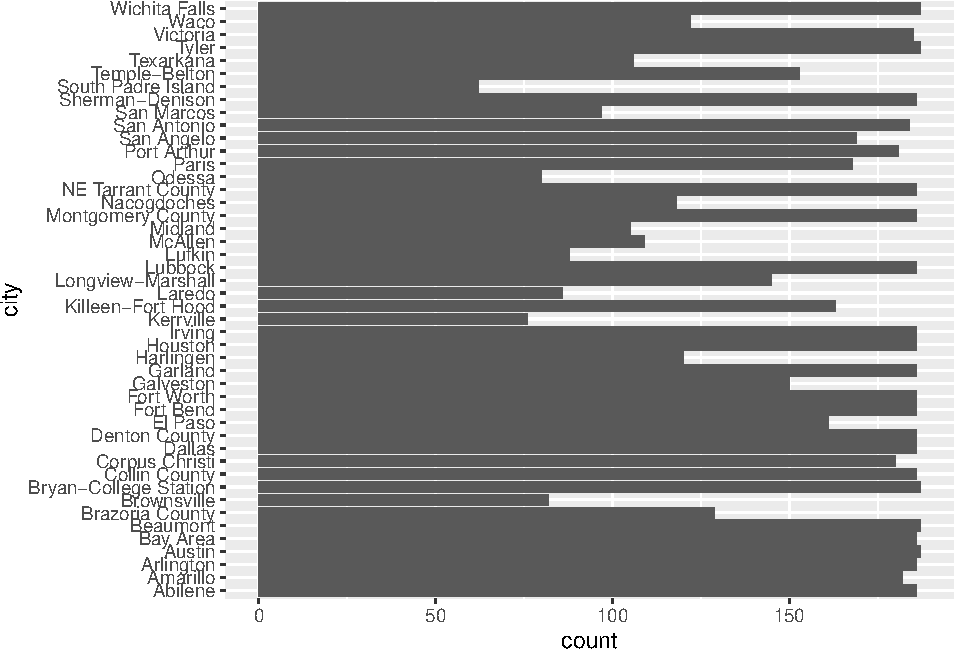
\includegraphics{code4stem_files/figure-latex/visualize txhousing-1.pdf}
Use recode() to create the new purpose\_recode variable

\begin{Shaded}
\begin{Highlighting}[]
\NormalTok{tx_housing}\OperatorTok{$}\NormalTok{city_recode <-}\StringTok{ }\NormalTok{tx_housing}\OperatorTok{$}\NormalTok{city }\OperatorTok
\StringTok{  }\KeywordTok{recode}\NormalTok{(}\StringTok{"Bay Area"}\NormalTok{ =}\StringTok{ "California"}\NormalTok{,}
         \StringTok{"El Paso"}\NormalTok{ =}\StringTok{ "California"}\NormalTok{)}
\end{Highlighting}
\end{Shaded}

Build a linear regression model, purpose\_recode\_model:

\begin{Shaded}
\begin{Highlighting}[]
\NormalTok{purpose_recode_model <-}\StringTok{ }\KeywordTok{lm}\NormalTok{(sales }\OperatorTok{~}\StringTok{ }\NormalTok{city_recode, }\DataTypeTok{data =}\NormalTok{ tx_housing)}

\CommentTok{# Examine results of purpose_recode_model}
\KeywordTok{summary}\NormalTok{(purpose_recode_model)}
\end{Highlighting}
\end{Shaded}

\begin{verbatim}
## 
## Call:
## lm(formula = sales ~ city_recode, data = tx_housing)
## 
## Residuals:
##     Min      1Q  Median      3Q     Max 
## -2938.1   -40.2    -2.5    30.5  3353.9 
## 
## Coefficients:
##                                  Estimate Std. Error t value Pr(>|t|)    
## (Intercept)                       150.462     23.162   6.496 8.80e-11 ***
## city_recodeAmarillo                87.680     32.936   2.662 0.007781 ** 
## city_recodeArlington              272.425     32.756   8.317  < 2e-16 ***
## city_recodeAustin                1846.227     32.712  56.438  < 2e-16 ***
## city_recodeBeaumont                26.596     32.712   0.813 0.416221    
## city_recodeBrazoria County        -62.400     36.194  -1.724 0.084743 .  
## city_recodeBrownsville            -92.975     41.873  -2.220 0.026425 *  
## city_recodeBryan-College Station   36.281     32.712   1.109 0.267428    
## city_recodeCalifornia             338.886     28.706  11.805  < 2e-16 ***
## city_recodeCollin County          931.871     32.756  28.449  < 2e-16 ***
## city_recodeCorpus Christi         194.427     33.028   5.887 4.12e-09 ***
## city_recodeDallas                4205.000     32.756 128.373  < 2e-16 ***
## city_recodeDenton County          476.242     32.756  14.539  < 2e-16 ***
## city_recodeFort Bend              669.758     32.756  20.447  < 2e-16 ***
## city_recodeFort Worth             622.441     32.756  19.002  < 2e-16 ***
## city_recodeGalveston              -65.862     34.666  -1.900 0.057484 .  
## city_recodeGarland                 42.683     32.756   1.303 0.192600    
## city_recodeHarlingen              -85.571     36.987  -2.314 0.020721 *  
## city_recodeHouston               5440.672     32.756 166.096  < 2e-16 ***
## city_recodeIrving                 -30.478     32.756  -0.930 0.352161    
## city_recodeKerrville             -106.291     43.005  -2.472 0.013475 *  
## city_recodeKilleen-Fort Hood       64.930     33.892   1.916 0.055430 .  
## city_recodeLaredo                 -61.776     41.192  -1.500 0.133732    
## city_recodeLongview-Marshall       35.689     34.995   1.020 0.307840    
## city_recodeLubbock                113.511     32.756   3.465 0.000533 ***
## city_recodeLufkin                -103.349     40.871  -2.529 0.011471 *  
## city_recodeMcAllen                  5.969     38.104   0.157 0.875530    
## city_recodeMidland                 -4.081     38.559  -0.106 0.915706    
## city_recodeMontgomery County      410.027     32.756  12.518  < 2e-16 ***
## city_recodeNacogdoches           -120.412     37.177  -3.239 0.001206 ** 
## city_recodeNE Tarrant County      532.387     32.756  16.253  < 2e-16 ***
## city_recodeOdessa                 -59.912     42.235  -1.419 0.156075    
## city_recodeParis                 -115.998     33.622  -3.450 0.000564 ***
## city_recodePort Arthur            -83.849     32.982  -2.542 0.011034 *  
## city_recodeSan Angelo             -37.368     33.570  -1.113 0.265688    
## city_recodeSan Antonio           1574.038     32.845  47.923  < 2e-16 ***
## city_recodeSan Marcos            -128.040     39.563  -3.236 0.001216 ** 
## city_recodeSherman-Denison        -46.134     32.756  -1.408 0.159050    
## city_recodeSouth Padre Island    -121.366     46.324  -2.620 0.008814 ** 
## city_recodeTemple-Belton          -19.992     34.477  -0.580 0.562030    
## city_recodeTexarkana              -73.142     38.443  -1.903 0.057132 .  
## city_recodeTyler                   97.971     32.712   2.995 0.002755 ** 
## city_recodeVictoria               -80.922     32.800  -2.467 0.013645 *  
## city_recodeWaco                    36.947     36.802   1.004 0.315437    
## city_recodeWichita Falls          -13.232     32.712  -0.405 0.685850    
## ---
## Signif. codes:  0 '***' 0.001 '**' 0.01 '*' 0.05 '.' 0.1 ' ' 1
## 
## Residual standard error: 315.9 on 7081 degrees of freedom
## Multiple R-squared:  0.9269,	Adjusted R-squared:  0.9264 
## F-statistic:  2040 on 44 and 7081 DF,  p-value: < 2.2e-16
\end{verbatim}

Get anova results and save as purpose\_recode\_anova:

\begin{Shaded}
\begin{Highlighting}[]
\NormalTok{purpose_recode_anova <-}\StringTok{ }\KeywordTok{anova}\NormalTok{(purpose_recode_model)}

\CommentTok{# Print purpose_recode_anova}
\NormalTok{purpose_recode_anova}
\end{Highlighting}
\end{Shaded}

\begin{verbatim}
## Analysis of Variance Table
## 
## Response: sales
##               Df     Sum Sq   Mean Sq F value    Pr(>F)    
## city_recode   44 8955309044 203529751  2039.7 < 2.2e-16 ***
## Residuals   7081  706580734     99785                      
## ---
## Signif. codes:  0 '***' 0.001 '**' 0.01 '*' 0.05 '.' 0.1 ' ' 1
\end{verbatim}

Examine class of purpose\_recode\_anova:

\begin{Shaded}
\begin{Highlighting}[]
\KeywordTok{class}\NormalTok{(purpose_recode_anova)}
\end{Highlighting}
\end{Shaded}

\begin{verbatim}
## [1] "anova"      "data.frame"
\end{verbatim}

Use aov() to build purpose\_aov:

\begin{Shaded}
\begin{Highlighting}[]
\CommentTok{# Analysis of variance}
\NormalTok{purpose_aov <-}\StringTok{ }\KeywordTok{aov}\NormalTok{(sales }\OperatorTok{~}\StringTok{ }\NormalTok{city_recode, }\DataTypeTok{data =}\NormalTok{ tx_housing)}
\end{Highlighting}
\end{Shaded}

Conduct Tukey's HSD test to create tukey\_output:

\begin{Shaded}
\begin{Highlighting}[]
\NormalTok{tukey_output <-}\StringTok{ }\KeywordTok{TukeyHSD}\NormalTok{(purpose_aov, }\StringTok{"city_recode"}\NormalTok{, }\DataTypeTok{conf.level =} \FloatTok{0.95}\NormalTok{)}

\CommentTok{# Tidy tukey_output to make sense of the results}
\KeywordTok{tidy}\NormalTok{(tukey_output)}
\end{Highlighting}
\end{Shaded}

\begin{verbatim}
## # A tibble: 990 x 7
##    term     contrast          null.value estimate conf.low conf.high adj.p.value
##    <chr>    <chr>                  <dbl>    <dbl>    <dbl>     <dbl>       <dbl>
##  1 city_re~ Amarillo-Abilene           0     87.7    -42.3     218.     8.41e- 1
##  2 city_re~ Arlington-Abilene          0    272.     143.      402.     8.51e-12
##  3 city_re~ Austin-Abilene             0   1846.    1717.     1975.     7.92e-12
##  4 city_re~ Beaumont-Abilene           0     26.6   -102.      156.     1.00e+ 0
##  5 city_re~ Brazoria County-~          0    -62.4   -205.       80.4    1.00e+ 0
##  6 city_re~ Brownsville-Abil~          0    -93.0   -258.       72.2    9.86e- 1
##  7 city_re~ Bryan-College St~          0     36.3    -92.8     165.     1.00e+ 0
##  8 city_re~ California-Abile~          0    339.     226.      452.     7.92e-12
##  9 city_re~ Collin County-Ab~          0    932.     803.     1061.     7.92e-12
## 10 city_re~ Corpus Christi-A~          0    194.      64.1     325.     4.00e- 6
## # ... with 980 more rows
\end{verbatim}

Multiple factor experiments:
Use aov() to build purpose\_emp\_aov

\begin{Shaded}
\begin{Highlighting}[]
\NormalTok{purpose_emp_aov <-}\StringTok{ }\KeywordTok{aov}\NormalTok{(sales }\OperatorTok{~}\StringTok{ }\NormalTok{city_recode }\OperatorTok{+}\StringTok{ }\NormalTok{volume , }\DataTypeTok{data =}\NormalTok{ tx_housing)}

\CommentTok{# Print purpose_emp_aov to the console}
\CommentTok{# purpose_emp_aov}

\CommentTok{#Call summary() to see the p-values:}
\KeywordTok{summary}\NormalTok{(purpose_emp_aov)}
\end{Highlighting}
\end{Shaded}

\begin{verbatim}
##               Df    Sum Sq   Mean Sq F value Pr(>F)    
## city_recode   44 8.955e+09 203529751   12992 <2e-16 ***
## volume         1 5.957e+08 595663462   38022 <2e-16 ***
## Residuals   7080 1.109e+08     15666                   
## ---
## Signif. codes:  0 '***' 0.001 '**' 0.01 '*' 0.05 '.' 0.1 ' ' 1
\end{verbatim}

Model validation
Pre-modeling exploratory data analysis
Examine the summary of sales

\begin{Shaded}
\begin{Highlighting}[]
\KeywordTok{summary}\NormalTok{(tx_housing}\OperatorTok{$}\NormalTok{sales)}
\end{Highlighting}
\end{Shaded}

\begin{verbatim}
##    Min. 1st Qu.  Median    Mean 3rd Qu.    Max. 
##       6      95     187     603     527    8945
\end{verbatim}

Examine sales by volume:

\begin{Shaded}
\begin{Highlighting}[]
\NormalTok{tx_housing }\OperatorTok\StringTok{ }
\StringTok{  }\KeywordTok{group_by}\NormalTok{(volume) }\OperatorTok\StringTok{ }
\StringTok{  }\KeywordTok{summarize}\NormalTok{(}\DataTypeTok{mean =} \KeywordTok{mean}\NormalTok{(sales), }\DataTypeTok{var =} \KeywordTok{var}\NormalTok{(sales), }\DataTypeTok{median =} \KeywordTok{median}\NormalTok{(sales))}
\end{Highlighting}
\end{Shaded}

\begin{verbatim}
## # A tibble: 6,855 x 4
##     volume  mean   var median
##      <dbl> <dbl> <dbl>  <dbl>
##  1  835000    14    NA     14
##  2 1018825    14    NA     14
##  3 1110000     9    NA      9
##  4 1156999     6    NA      6
##  5 1165000    18    NA     18
##  6 1215000    11    NA     11
##  7 1260000    23    NA     23
##  8 1305000    16    NA     16
##  9 1419500    25    NA     25
## 10 1434950    22    NA     22
## # ... with 6,845 more rows
\end{verbatim}

Make a boxplot of sales by volume

\begin{Shaded}
\begin{Highlighting}[]
\KeywordTok{ggplot}\NormalTok{(tx_housing, }\KeywordTok{aes}\NormalTok{(}\DataTypeTok{x =}\NormalTok{ volume, }\DataTypeTok{y =}\NormalTok{ sales)) }\OperatorTok{+}\StringTok{ }
\StringTok{  }\KeywordTok{geom_boxplot}\NormalTok{()}
\end{Highlighting}
\end{Shaded}

\begin{verbatim}
## Warning: Continuous x aesthetic -- did you forget aes(group=...)?
\end{verbatim}

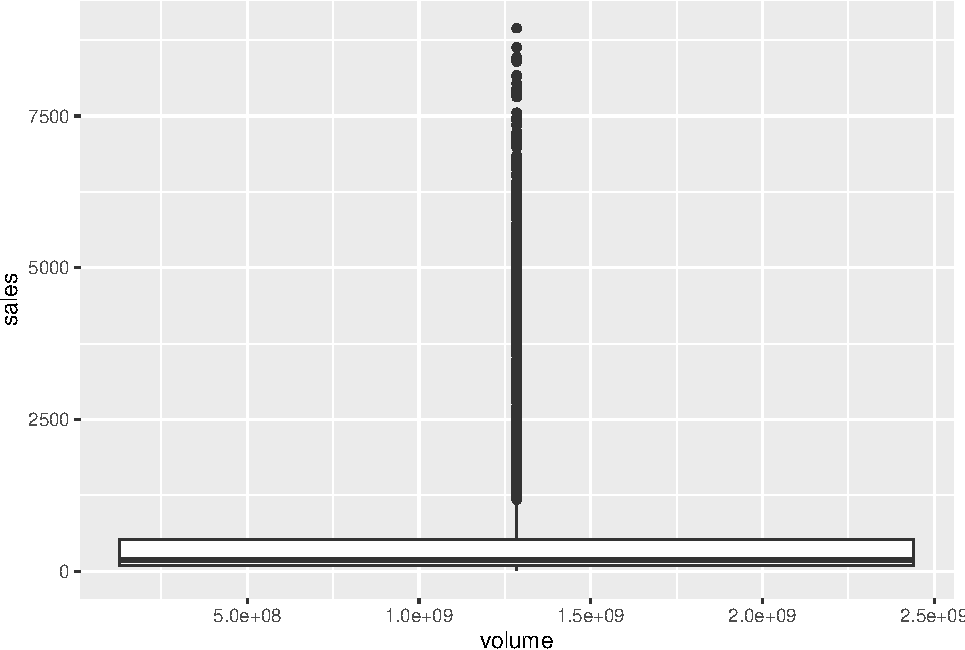
\includegraphics{code4stem_files/figure-latex/box plot of sales a/b test-1.pdf}

Use aov() to create volume\_aov plus call summary() to print results

\begin{Shaded}
\begin{Highlighting}[]
\NormalTok{volume_aov <-}\StringTok{ }\KeywordTok{aov}\NormalTok{(volume }\OperatorTok{~}\StringTok{ }\NormalTok{sales, }\DataTypeTok{data =}\NormalTok{ tx_housing)}
\KeywordTok{summary}\NormalTok{(volume_aov)}
\end{Highlighting}
\end{Shaded}

\begin{verbatim}
##               Df    Sum Sq   Mean Sq F value Pr(>F)    
## sales          1 4.535e+20 4.535e+20  180283 <2e-16 ***
## Residuals   7124 1.792e+19 2.515e+15                   
## ---
## Signif. codes:  0 '***' 0.001 '**' 0.01 '*' 0.05 '.' 0.1 ' ' 1
\end{verbatim}

Post-modeling validation plots + variance
For a 2x2 grid of plots:

\begin{Shaded}
\begin{Highlighting}[]
\KeywordTok{par}\NormalTok{(}\DataTypeTok{mfrow =} \KeywordTok{c}\NormalTok{(}\DecValTok{2}\NormalTok{, }\DecValTok{2}\NormalTok{))}

\CommentTok{# Plot grade_aov}
\KeywordTok{plot}\NormalTok{(volume_aov)}
\end{Highlighting}
\end{Shaded}

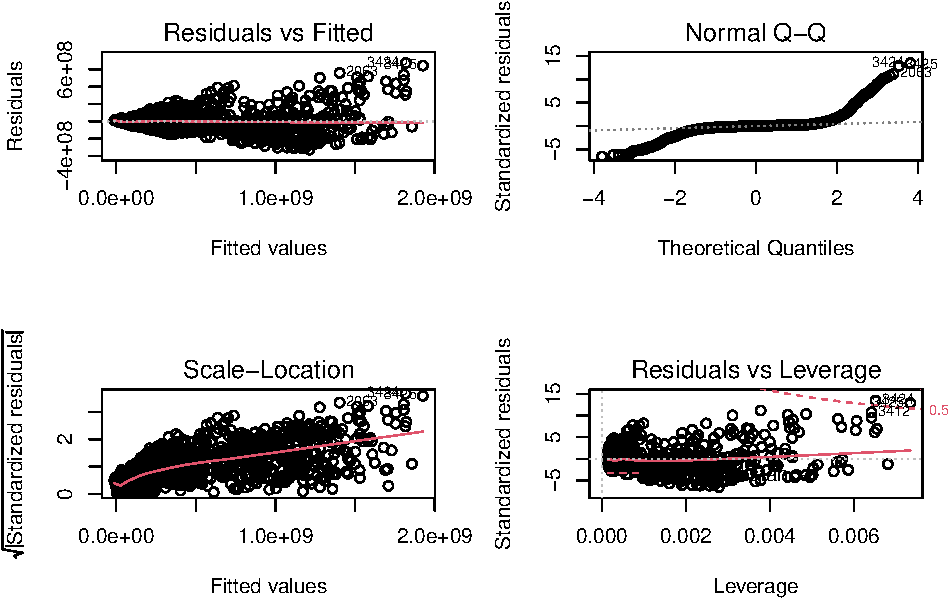
\includegraphics{code4stem_files/figure-latex/qq plots-1.pdf}

Bartlett's test for homogeneity of variance
We can test for homogeneity of variances using bartlett.test(), which takes a formula and a dataset as inputs:
- bartlett.test(volume \textasciitilde{} sales, data = tx\_housing)

Conduct the Kruskal-Wallis rank sum test:
kruskal.test() to examine whether volume varies by sales when a non-parametric model is employed

\begin{Shaded}
\begin{Highlighting}[]
\KeywordTok{kruskal.test}\NormalTok{(volume }\OperatorTok{~}\StringTok{ }\NormalTok{sales,}
             \DataTypeTok{data =}\NormalTok{ tx_housing)}
\end{Highlighting}
\end{Shaded}

\begin{verbatim}
## 
## 	Kruskal-Wallis rank sum test
## 
## data:  volume by sales
## Kruskal-Wallis chi-squared = 6877.9, df = 1702, p-value < 2.2e-16
\end{verbatim}

The low p-value indicates that based on this test, we can be confident in our result, which we found across this experiment, that volume varies by sales

Sampling {[}randomized experiments{]}

load data from NHANES dataset
\url{https://wwwn.cdc.gov/nchs/nhanes/continuousnhanes/default.aspx?BeginYear=2015}

Import the three datasets using read\_xpt():

\begin{Shaded}
\begin{Highlighting}[]
\NormalTok{nhanes_demo <-}\StringTok{ }\KeywordTok{read_xpt}\NormalTok{(}\KeywordTok{url}\NormalTok{(}\StringTok{"https://wwwn.cdc.gov/Nchs/Nhanes/2015-2016/DEMO_I.XPT"}\NormalTok{))}
\NormalTok{nhanes_bodymeasures <-}\StringTok{ }\KeywordTok{read_xpt}\NormalTok{(}\KeywordTok{url}\NormalTok{(}\StringTok{"https://wwwn.cdc.gov/Nchs/Nhanes/2015-2016/BMX_I.XPT"}\NormalTok{))}
\NormalTok{nhanes_medical <-}\StringTok{ }\KeywordTok{read_xpt}\NormalTok{(}\KeywordTok{url}\NormalTok{(}\StringTok{"https://wwwn.cdc.gov/Nchs/Nhanes/2015-2016/MCQ_I.XPT"}\NormalTok{))}
\end{Highlighting}
\end{Shaded}

Merge the 3 datasets you just created to create nhanes\_combined:

\begin{Shaded}
\begin{Highlighting}[]
\NormalTok{nhanes_combined <-}\StringTok{ }\KeywordTok{list}\NormalTok{(nhanes_demo, nhanes_medical, nhanes_bodymeasures) }\OperatorTok
\StringTok{  }\KeywordTok{Reduce}\NormalTok{(}\ControlFlowTok{function}\NormalTok{(df1, df2) }\KeywordTok{inner_join}\NormalTok{(df1, df2, }\DataTypeTok{by =} \StringTok{"SEQN"}\NormalTok{), .)}
\end{Highlighting}
\end{Shaded}

Fill in the dplyr code:

\begin{Shaded}
\begin{Highlighting}[]
\NormalTok{nhanes_combined }\OperatorTok\StringTok{ }
\StringTok{  }\KeywordTok{group_by}\NormalTok{(MCQ035) }\OperatorTok\StringTok{ }
\StringTok{  }\KeywordTok{summarize}\NormalTok{(}\DataTypeTok{mean =} \KeywordTok{mean}\NormalTok{(INDHHIN2, }\DataTypeTok{na.rm =} \OtherTok{TRUE}\NormalTok{))}
\end{Highlighting}
\end{Shaded}

\begin{verbatim}
## # A tibble: 4 x 2
##   MCQ035  mean
##    <dbl> <dbl>
## 1      1  9.89
## 2      2 10.4 
## 3      9 17.8 
## 4     NA 11.7
\end{verbatim}

Fill in the ggplot2 code:

\begin{Shaded}
\begin{Highlighting}[]
\NormalTok{nhanes_combined }\OperatorTok\StringTok{ }
\StringTok{  }\KeywordTok{ggplot}\NormalTok{(}\KeywordTok{aes}\NormalTok{(}\KeywordTok{as.factor}\NormalTok{(MCQ035), INDHHIN2)) }\OperatorTok{+}
\StringTok{  }\KeywordTok{geom_boxplot}\NormalTok{() }\OperatorTok{+}
\StringTok{  }\KeywordTok{labs}\NormalTok{(}\DataTypeTok{x =} \StringTok{"Disease type"}\NormalTok{,}
       \DataTypeTok{y =} \StringTok{"Income"}\NormalTok{)}
\end{Highlighting}
\end{Shaded}

\begin{verbatim}
## Warning: Removed 273 rows containing non-finite values (stat_boxplot).
\end{verbatim}

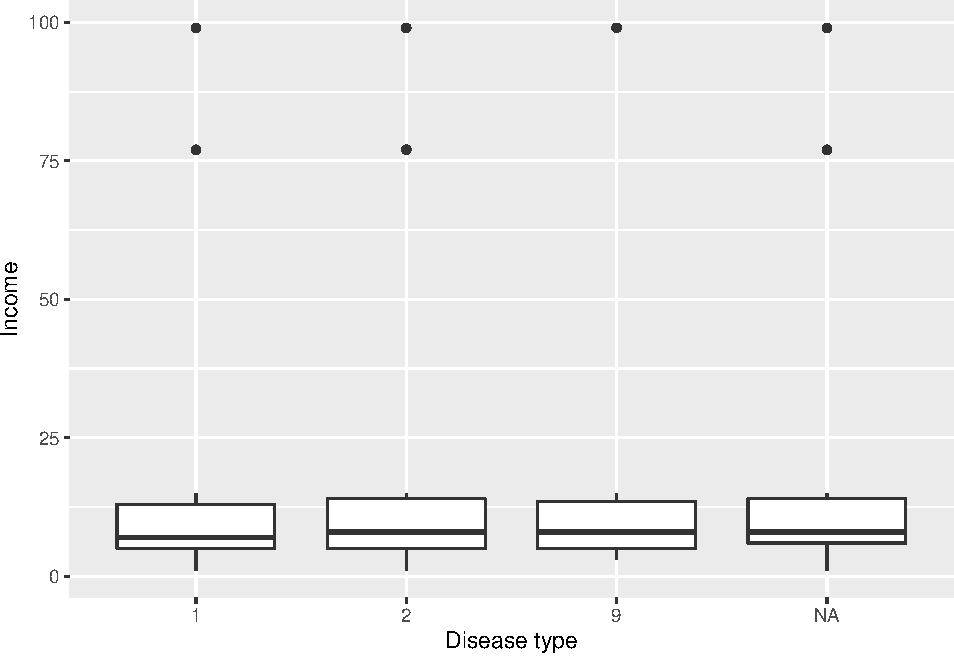
\includegraphics{code4stem_files/figure-latex/plot data-1.pdf}

NHANES Data Cleaning
Filter to keep only those greater than 16:

\begin{Shaded}
\begin{Highlighting}[]
\NormalTok{nhanes_filter <-}\StringTok{ }\NormalTok{nhanes_combined }\OperatorTok\StringTok{ }\KeywordTok{filter}\NormalTok{(RIDAGEYR }\OperatorTok{>}\StringTok{ }\DecValTok{16}\NormalTok{)}
\end{Highlighting}
\end{Shaded}

Load simputation \& impute bmxwt by riagendr: library(simputation)

\begin{Shaded}
\begin{Highlighting}[]
\NormalTok{nhanes_final <-}\StringTok{ }\NormalTok{simputation}\OperatorTok{::}\KeywordTok{impute_median}\NormalTok{(nhanes_filter, INDHHIN2 }\OperatorTok{~}\StringTok{ }\NormalTok{RIDAGEYR)}
\end{Highlighting}
\end{Shaded}

Recode mcq365d with recode() \& examine with count():

\begin{Shaded}
\begin{Highlighting}[]
\NormalTok{nhanes_final}\OperatorTok{$}\NormalTok{mcq365d <-}\StringTok{ }\KeywordTok{recode}\NormalTok{(nhanes_final}\OperatorTok{$}\NormalTok{MCQ035, }
                               \StringTok{`}\DataTypeTok{1}\StringTok{`}\NormalTok{ =}\StringTok{ }\DecValTok{1}\NormalTok{,}
                               \StringTok{`}\DataTypeTok{2}\StringTok{`}\NormalTok{ =}\StringTok{ }\DecValTok{2}\NormalTok{,}
                               \StringTok{`}\DataTypeTok{9}\StringTok{`}\NormalTok{ =}\StringTok{ }\DecValTok{2}\NormalTok{)}
\NormalTok{nhanes_final }\OperatorTok\StringTok{ }\KeywordTok{count}\NormalTok{(MCQ035)}
\end{Highlighting}
\end{Shaded}

\begin{verbatim}
## # A tibble: 4 x 2
##   MCQ035     n
##    <dbl> <int>
## 1      1   522
## 2      2   369
## 3      9    15
## 4     NA  4981
\end{verbatim}

Resampling NHANES data:
Use sample\_n() to create nhanes\_srs:

\begin{Shaded}
\begin{Highlighting}[]
\NormalTok{nhanes_srs <-}\StringTok{ }\NormalTok{nhanes_final }\OperatorTok\StringTok{ }\KeywordTok{sample_n}\NormalTok{(}\DecValTok{2500}\NormalTok{)}
\end{Highlighting}
\end{Shaded}

Create nhanes\_stratified with group\_by() and sample\_n()

\begin{Shaded}
\begin{Highlighting}[]
\NormalTok{nhanes_stratified <-}\StringTok{ }\NormalTok{nhanes_final }\OperatorTok\StringTok{ }\KeywordTok{group_by}\NormalTok{(RIDAGEYR) }\OperatorTok\StringTok{ }\KeywordTok{sample_n}\NormalTok{(}\DecValTok{2000}\NormalTok{, }\DataTypeTok{replace =} \OtherTok{TRUE}\NormalTok{)}

\NormalTok{nhanes_stratified }\OperatorTok\StringTok{ }
\StringTok{  }\KeywordTok{count}\NormalTok{(RIDAGEYR)}
\end{Highlighting}
\end{Shaded}

\begin{verbatim}
## # A tibble: 64 x 2
## # Groups:   RIDAGEYR [64]
##    RIDAGEYR     n
##       <dbl> <int>
##  1       17  2000
##  2       18  2000
##  3       19  2000
##  4       20  2000
##  5       21  2000
##  6       22  2000
##  7       23  2000
##  8       24  2000
##  9       25  2000
## 10       26  2000
## # ... with 54 more rows
\end{verbatim}

Load sampling package and create nhanes\_cluster with cluster(): library(sampling)

\begin{Shaded}
\begin{Highlighting}[]
\NormalTok{nhanes_cluster <-}\StringTok{ }\KeywordTok{cluster}\NormalTok{(nhanes_final, }\KeywordTok{c}\NormalTok{(}\StringTok{"INDHHIN2"}\NormalTok{), }\DecValTok{6}\NormalTok{, }\DataTypeTok{method =} \StringTok{"srswor"}\NormalTok{)}
\end{Highlighting}
\end{Shaded}

Randomized complete block designs (RCBD): use library(agricolae)
block = experimental groups are blocked to be similar (e.g.~by sex)
complete = each treatment is used the same of times in every block
randomized = the treatment is assigned randomly inside each block

Create designs using ls():

\begin{Shaded}
\begin{Highlighting}[]
\NormalTok{designs <-}\StringTok{ }\KeywordTok{ls}\NormalTok{(}\StringTok{"package:agricolae"}\NormalTok{, }\DataTypeTok{pattern =} \StringTok{"design"}\NormalTok{)}
\KeywordTok{print}\NormalTok{(designs)}
\end{Highlighting}
\end{Shaded}

\begin{verbatim}
##  [1] "design.ab"      "design.alpha"   "design.bib"     "design.crd"    
##  [5] "design.cyclic"  "design.dau"     "design.graeco"  "design.lattice"
##  [9] "design.lsd"     "design.mat"     "design.rcbd"    "design.split"  
## [13] "design.strip"   "design.youden"
\end{verbatim}

Use str() to view design.rcbd's criteria:

\begin{Shaded}
\begin{Highlighting}[]
\KeywordTok{str}\NormalTok{(design.rcbd)}
\end{Highlighting}
\end{Shaded}

\begin{verbatim}
## function (trt, r, serie = 2, seed = 0, kinds = "Super-Duper", first = TRUE, 
##     continue = FALSE, randomization = TRUE)
\end{verbatim}

Build treats and rep

\begin{Shaded}
\begin{Highlighting}[]
\NormalTok{treats <-}\StringTok{ }\NormalTok{LETTERS[}\DecValTok{1}\OperatorTok{:}\DecValTok{5}\NormalTok{]}
\NormalTok{blocks <-}\StringTok{ }\DecValTok{4}
\NormalTok{blocks}
\end{Highlighting}
\end{Shaded}

\begin{verbatim}
## [1] 4
\end{verbatim}

NHANES RCBD:
Build my\_design\_rcbd and view the sketch

\begin{Shaded}
\begin{Highlighting}[]
\NormalTok{my_design_rcbd <-}\StringTok{ }\KeywordTok{design.rcbd}\NormalTok{(treats, }\DataTypeTok{r =}\NormalTok{ blocks, }\DataTypeTok{seed =} \DecValTok{42}\NormalTok{)}
\NormalTok{my_design_rcbd}\OperatorTok{$}\NormalTok{sketch}
\end{Highlighting}
\end{Shaded}

\begin{verbatim}
##      [,1] [,2] [,3] [,4] [,5]
## [1,] "D"  "A"  "C"  "B"  "E" 
## [2,] "E"  "A"  "C"  "D"  "B" 
## [3,] "D"  "B"  "E"  "A"  "C" 
## [4,] "B"  "D"  "E"  "C"  "A"
\end{verbatim}

Use aov() to create nhanes\_rcbd:

\begin{Shaded}
\begin{Highlighting}[]
\NormalTok{nhanes_rcbd <-}\StringTok{ }\KeywordTok{aov}\NormalTok{(INDHHIN2 }\OperatorTok{~}\StringTok{ }\NormalTok{MCQ035 }\OperatorTok{+}\StringTok{ }\NormalTok{RIDAGEYR, }\DataTypeTok{data =}\NormalTok{ nhanes_final)}
\end{Highlighting}
\end{Shaded}

Check results of nhanes\_rcbd with summary():

\begin{Shaded}
\begin{Highlighting}[]
\KeywordTok{summary}\NormalTok{(nhanes_rcbd)}
\end{Highlighting}
\end{Shaded}

\begin{verbatim}
##              Df Sum Sq Mean Sq F value  Pr(>F)   
## MCQ035        1   1399  1398.5   8.242 0.00419 **
## RIDAGEYR      1    312   312.4   1.841 0.17519   
## Residuals   903 153221   169.7                   
## ---
## Signif. codes:  0 '***' 0.001 '**' 0.01 '*' 0.05 '.' 0.1 ' ' 1
## 4981 observations deleted due to missingness
\end{verbatim}

Print mean weights by mcq365d and riagendr:

\begin{Shaded}
\begin{Highlighting}[]
\NormalTok{nhanes_final }\OperatorTok\StringTok{ }
\StringTok{  }\KeywordTok{group_by}\NormalTok{(MCQ035, RIDAGEYR) }\OperatorTok\StringTok{ }
\StringTok{  }\KeywordTok{summarize}\NormalTok{(}\DataTypeTok{mean_ind =} \KeywordTok{mean}\NormalTok{(INDHHIN2, }\DataTypeTok{na.rm =} \OtherTok{TRUE}\NormalTok{))}
\end{Highlighting}
\end{Shaded}

\begin{verbatim}
## # A tibble: 204 x 3
## # Groups:   MCQ035 [4]
##    MCQ035 RIDAGEYR mean_ind
##     <dbl>    <dbl>    <dbl>
##  1      1       17    10.3 
##  2      1       18     8   
##  3      1       19     5.38
##  4      1       20     8   
##  5      1       21     8.75
##  6      1       22     6.27
##  7      1       23     7.18
##  8      1       24    14   
##  9      1       25     9.11
## 10      1       26    10.6 
## # ... with 194 more rows
\end{verbatim}

RCBD Model Validation
Set up the 2x2 plotting grid and plot nhanes\_rcbd

\begin{Shaded}
\begin{Highlighting}[]
\KeywordTok{par}\NormalTok{(}\DataTypeTok{mfrow =} \KeywordTok{c}\NormalTok{(}\DecValTok{2}\NormalTok{, }\DecValTok{2}\NormalTok{))}
\KeywordTok{plot}\NormalTok{(nhanes_rcbd)}
\end{Highlighting}
\end{Shaded}

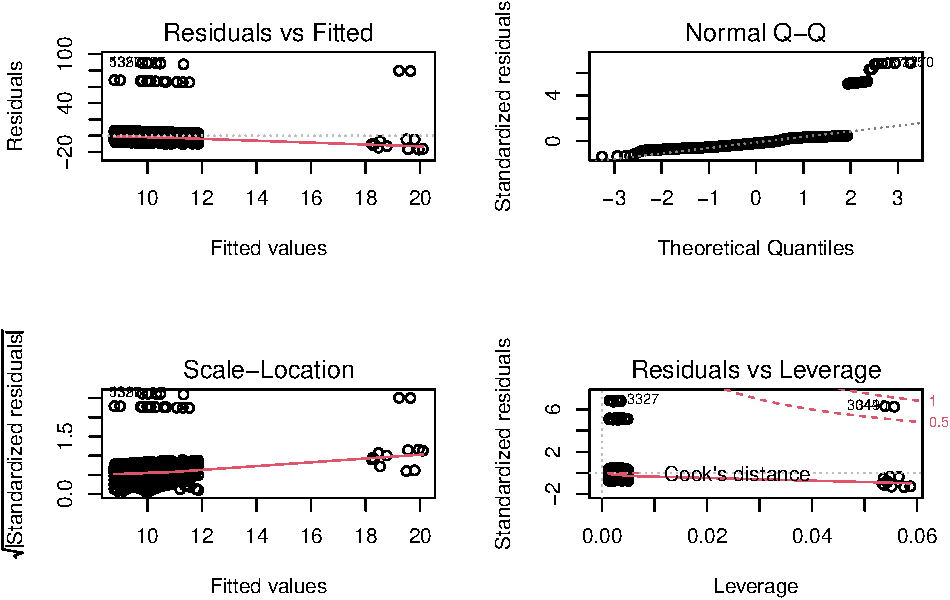
\includegraphics{code4stem_files/figure-latex/2x2 grid-1.pdf}

Run the code to view the interaction plots:

\begin{Shaded}
\begin{Highlighting}[]
\KeywordTok{with}\NormalTok{(nhanes_final, }\KeywordTok{interaction.plot}\NormalTok{(MCQ035, RIDAGEYR, INDHHIN2))}
\end{Highlighting}
\end{Shaded}

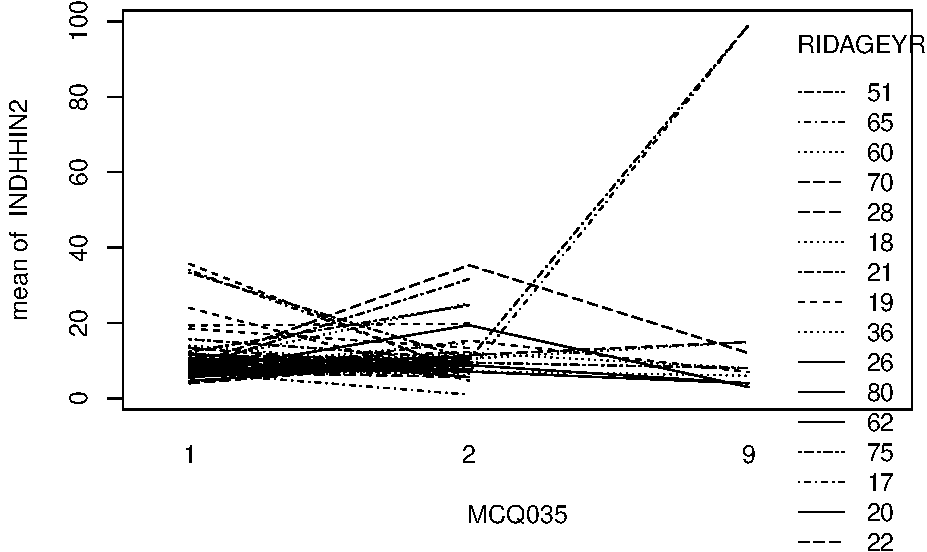
\includegraphics{code4stem_files/figure-latex/view final-1.pdf}

Balanced incomplete block design (BIBD)
Balanced = each pair of treatment occur together in a block an equal of times
Incomplete = not every treatment will appear in every block

Use str() to view design.bibd's criteria
str(design.bib)

Columns are a blocking factor

create my\_design\_bibd\_1

\begin{Shaded}
\begin{Highlighting}[]
\NormalTok{my_design_bibd_}\DecValTok{1}\NormalTok{ <-}\StringTok{ }\NormalTok{agricolae}\OperatorTok{::}\KeywordTok{design.bib}\NormalTok{(LETTERS[}\DecValTok{1}\OperatorTok{:}\DecValTok{3}\NormalTok{], }\DataTypeTok{k =} \DecValTok{3}\NormalTok{, }\DataTypeTok{seed =} \DecValTok{42}\NormalTok{)}
\end{Highlighting}
\end{Shaded}

\begin{verbatim}
## 
## Parameters BIB
## ==============
## Lambda     : 2
## treatmeans : 3
## Block size : 3
## Blocks     : 2
## Replication: 2 
## 
## Efficiency factor 1 
## 
## <<< Book >>>
\end{verbatim}

create my\_design\_bibd\_2

\begin{Shaded}
\begin{Highlighting}[]
\NormalTok{my_design_bibd_}\DecValTok{2}\NormalTok{ <-}\StringTok{ }\KeywordTok{design.bib}\NormalTok{(LETTERS[}\DecValTok{1}\OperatorTok{:}\DecValTok{8}\NormalTok{], }\DataTypeTok{k =} \DecValTok{8}\NormalTok{, }\DataTypeTok{seed =} \DecValTok{42}\NormalTok{)}
\end{Highlighting}
\end{Shaded}

\begin{verbatim}
## 
## Parameters BIB
## ==============
## Lambda     : 2
## treatmeans : 8
## Block size : 8
## Blocks     : 2
## Replication: 2 
## 
## Efficiency factor 1 
## 
## <<< Book >>>
\end{verbatim}

create my\_design\_bibd\_3:

\begin{Shaded}
\begin{Highlighting}[]
\NormalTok{my_design_bibd_}\DecValTok{3}\NormalTok{ <-}\StringTok{ }\KeywordTok{design.bib}\NormalTok{(LETTERS[}\DecValTok{1}\OperatorTok{:}\DecValTok{4}\NormalTok{], }\DataTypeTok{k =} \DecValTok{4}\NormalTok{, }\DataTypeTok{seed =} \DecValTok{42}\NormalTok{)}
\end{Highlighting}
\end{Shaded}

\begin{verbatim}
## 
## Parameters BIB
## ==============
## Lambda     : 2
## treatmeans : 4
## Block size : 4
## Blocks     : 2
## Replication: 2 
## 
## Efficiency factor 1 
## 
## <<< Book >>>
\end{verbatim}

\begin{Shaded}
\begin{Highlighting}[]
\NormalTok{my_design_bibd_}\DecValTok{3}\OperatorTok{$}\NormalTok{sketch}
\end{Highlighting}
\end{Shaded}

\begin{verbatim}
##      [,1] [,2] [,3] [,4]
## [1,] "C"  "A"  "D"  "B" 
## [2,] "C"  "D"  "B"  "A"
\end{verbatim}

Build the data.frame:

\begin{Shaded}
\begin{Highlighting}[]
\NormalTok{creatinine <-}\StringTok{ }\KeywordTok{c}\NormalTok{(}\FloatTok{1.98}\NormalTok{, }\FloatTok{1.97}\NormalTok{, }\FloatTok{2.35}\NormalTok{, }\FloatTok{2.09}\NormalTok{, }\FloatTok{1.87}\NormalTok{, }\FloatTok{1.95}\NormalTok{, }\FloatTok{2.08}\NormalTok{, }\FloatTok{2.01}\NormalTok{, }\FloatTok{1.84}\NormalTok{, }\FloatTok{2.06}\NormalTok{, }\FloatTok{1.97}\NormalTok{, }\FloatTok{2.22}\NormalTok{)}
\NormalTok{food <-}\StringTok{ }\KeywordTok{as.factor}\NormalTok{(}\KeywordTok{c}\NormalTok{(}\StringTok{"A"}\NormalTok{, }\StringTok{"C"}\NormalTok{, }\StringTok{"D"}\NormalTok{, }\StringTok{"A"}\NormalTok{, }\StringTok{"B"}\NormalTok{, }\StringTok{"C"}\NormalTok{, }\StringTok{"B"}\NormalTok{, }\StringTok{"C"}\NormalTok{, }\StringTok{"D"}\NormalTok{, }\StringTok{"A"}\NormalTok{, }\StringTok{"B"}\NormalTok{, }\StringTok{"D"}\NormalTok{))}
\NormalTok{color <-}\StringTok{ }\KeywordTok{as.factor}\NormalTok{(}\KeywordTok{rep}\NormalTok{(}\KeywordTok{c}\NormalTok{(}\StringTok{"Black"}\NormalTok{, }\StringTok{"White"}\NormalTok{, }\StringTok{"Orange"}\NormalTok{, }\StringTok{"Spotted"}\NormalTok{), }\DataTypeTok{each =} \DecValTok{3}\NormalTok{))}
\NormalTok{cat_experiment <-}\StringTok{ }\KeywordTok{as.data.frame}\NormalTok{(}\KeywordTok{cbind}\NormalTok{(creatinine, food, color))}
\end{Highlighting}
\end{Shaded}

Create cat\_model and examine with summary():

\begin{Shaded}
\begin{Highlighting}[]
\NormalTok{cat_model <-}\StringTok{ }\KeywordTok{aov}\NormalTok{(creatinine }\OperatorTok{~}\StringTok{ }\NormalTok{food }\OperatorTok{+}\StringTok{ }\NormalTok{color, }\DataTypeTok{data =}\NormalTok{ cat_experiment)}
\KeywordTok{summary}\NormalTok{(cat_model)}
\end{Highlighting}
\end{Shaded}

\begin{verbatim}
##             Df  Sum Sq  Mean Sq F value Pr(>F)
## food         1 0.01204 0.012042   0.530  0.485
## color        1 0.00697 0.006971   0.307  0.593
## Residuals    9 0.20461 0.022735
\end{verbatim}

Calculate lambda, where lamdba is a measure of proportional reduction in error in cross tabulation analysis:

\begin{Shaded}
\begin{Highlighting}[]
\NormalTok{DescTools}\OperatorTok{::}\KeywordTok{Lambda}\NormalTok{(cat_experiment, }\DataTypeTok{direction =} \KeywordTok{c}\NormalTok{(}\StringTok{"symmetric"}\NormalTok{, }\StringTok{"row"}\NormalTok{, }\StringTok{"column"}\NormalTok{), }\DataTypeTok{conf.level =} \OtherTok{NA}\NormalTok{)}
\end{Highlighting}
\end{Shaded}

\begin{verbatim}
## [1] 0.08636925
\end{verbatim}

Create weightlift\_model \& examine results:

\begin{Shaded}
\begin{Highlighting}[]
\NormalTok{weightlift_model <-}\StringTok{ }\KeywordTok{aov}\NormalTok{(MCQ035 }\OperatorTok{~}\StringTok{ }\NormalTok{INDHHIN2 }\OperatorTok{+}\StringTok{ }\NormalTok{RIDAGEYR, }\DataTypeTok{data =}\NormalTok{ nhanes_final)}
\KeywordTok{summary}\NormalTok{(weightlift_model)}
\end{Highlighting}
\end{Shaded}

\begin{verbatim}
##              Df Sum Sq Mean Sq F value  Pr(>F)   
## INDHHIN2      1    9.6   9.614   8.256 0.00416 **
## RIDAGEYR      1    3.9   3.868   3.321 0.06872 . 
## Residuals   903 1051.6   1.165                   
## ---
## Signif. codes:  0 '***' 0.001 '**' 0.01 '*' 0.05 '.' 0.1 ' ' 1
## 4981 observations deleted due to missingness
\end{verbatim}

Latin Squares Design
Key assumption: the treatment and two blocking factors do NOT interact
Two blocking factors (instead of one)
Analyze like RCBD

Mean, var, and median of Math score by Borough:

\begin{Shaded}
\begin{Highlighting}[]
\NormalTok{sat_scores <-}\StringTok{ }\KeywordTok{read.csv}\NormalTok{(}\KeywordTok{url}\NormalTok{(}\StringTok{"https://data.ct.gov/api/views/kbxi-4ia7/rows.csv?accessType=DOWNLOAD"}\NormalTok{))}

\NormalTok{sat_scores }\OperatorTok
\StringTok{  }\KeywordTok{group_by}\NormalTok{(District, Test.takers..}\DecValTok{2012}\NormalTok{) }\OperatorTok\StringTok{ }
\StringTok{  }\KeywordTok{summarize}\NormalTok{(}\DataTypeTok{mean =} \KeywordTok{mean}\NormalTok{(Test.takers..}\DecValTok{2012}\NormalTok{, }\DataTypeTok{na.rm =} \OtherTok{TRUE}\NormalTok{),}
            \DataTypeTok{var =} \KeywordTok{var}\NormalTok{(Test.takers..}\DecValTok{2012}\NormalTok{, }\DataTypeTok{na.rm =} \OtherTok{TRUE}\NormalTok{),}
            \DataTypeTok{median =} \KeywordTok{median}\NormalTok{(Test.takers..}\DecValTok{2012}\NormalTok{, }\DataTypeTok{na.rm =} \OtherTok{TRUE}\NormalTok{)) }\OperatorTok
\StringTok{  }\KeywordTok{head}\NormalTok{()}
\end{Highlighting}
\end{Shaded}

\begin{verbatim}
## # A tibble: 6 x 5
## # Groups:   District [6]
##   District                 Test.takers..2012  mean   var median
##   <chr>                                <int> <dbl> <dbl>  <dbl>
## 1 Amistad Academy District                34    34    NA     34
## 2 Ansonia                                118   118    NA    118
## 3 Avon                                   254   254    NA    254
## 4 Berlin                                 216   216    NA    216
## 5 Bethel                                 200   200    NA    200
## 6 Bloomfield                              14    14    NA     14
\end{verbatim}

Dealing with Missing Test Scores
Examine missingness with miss\_var\_summary() and library(mice):

\begin{Shaded}
\begin{Highlighting}[]
\NormalTok{sat_scores }\OperatorTok\StringTok{ }\KeywordTok{miss_var_summary}\NormalTok{()}
\end{Highlighting}
\end{Shaded}

\begin{verbatim}
## # A tibble: 12 x 3
##    variable                               n_miss pct_miss
##    <chr>                                   <int>    <dbl>
##  1 Test.takers..2013                           9     4.57
##  2 Test.takers..Change.                        9     4.57
##  3 Participation.Rate..estimate...Change.      8     4.06
##  4 Percent.Meeting.Benchmark..Change.          8     4.06
##  5 Test.takers..2012                           7     3.55
##  6 Participation.Rate..estimate...2012         7     3.55
##  7 Participation.Rate..estimate...2013         7     3.55
##  8 Percent.Meeting.Benchmark..2012             7     3.55
##  9 Percent.Meeting.Benchmark..2013             7     3.55
## 10 District.Number                             0     0   
## 11 District                                    0     0   
## 12 School                                      0     0
\end{verbatim}

\begin{Shaded}
\begin{Highlighting}[]
\NormalTok{sat_scores <-}\StringTok{ }\KeywordTok{na.omit}\NormalTok{(sat_scores)}

\NormalTok{mice}\OperatorTok{::}\KeywordTok{md.pattern}\NormalTok{(sat_scores)}
\end{Highlighting}
\end{Shaded}

\begin{verbatim}
##  /\     /\
## {  `---'  }
## {  O   O  }
## ==>  V <==  No need for mice. This data set is completely observed.
##  \  \|/  /
##   `-----'
\end{verbatim}

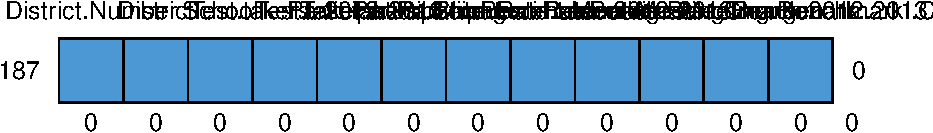
\includegraphics{code4stem_files/figure-latex/Examine missingness with md.pattern()-1.pdf}

\begin{verbatim}
##     District.Number District School Test.takers..2012 Test.takers..2013
## 187               1        1      1                 1                 1
##                   0        0      0                 0                 0
##     Test.takers..Change. Participation.Rate..estimate...2012
## 187                    1                                   1
##                        0                                   0
##     Participation.Rate..estimate...2013 Participation.Rate..estimate...Change.
## 187                                   1                                      1
##                                       0                                      0
##     Percent.Meeting.Benchmark..2012 Percent.Meeting.Benchmark..2013
## 187                               1                               1
##                                   0                               0
##     Percent.Meeting.Benchmark..Change.  
## 187                                  1 0
##                                      0 0
\end{verbatim}

Impute the Math score by Borough:

\begin{Shaded}
\begin{Highlighting}[]
\NormalTok{sat_scores_}\DecValTok{2}\NormalTok{ <-}\StringTok{ }\NormalTok{simputation}\OperatorTok{::}\KeywordTok{impute_median}\NormalTok{(sat_scores, Test.takers..}\DecValTok{2012} \OperatorTok{~}\StringTok{ }\NormalTok{District)}
\CommentTok{#Convert Math score to numeric}
\NormalTok{sat_scores}\OperatorTok{$}\NormalTok{Average_testtakers2012 <-}\StringTok{ }\KeywordTok{as.numeric}\NormalTok{(sat_scores}\OperatorTok{$}\NormalTok{Test.takers..}\DecValTok{2012}\NormalTok{)}
\end{Highlighting}
\end{Shaded}

Examine scores by Borough in both datasets, before and after imputation:

\begin{Shaded}
\begin{Highlighting}[]
\NormalTok{sat_scores }\OperatorTok\StringTok{ }
\StringTok{  }\KeywordTok{group_by}\NormalTok{(District) }\OperatorTok\StringTok{ }
\StringTok{  }\KeywordTok{summarize}\NormalTok{(}\DataTypeTok{median =} \KeywordTok{median}\NormalTok{(Test.takers..}\DecValTok{2012}\NormalTok{, }\DataTypeTok{na.rm =} \OtherTok{TRUE}\NormalTok{), }
            \DataTypeTok{mean =} \KeywordTok{mean}\NormalTok{(Test.takers..}\DecValTok{2012}\NormalTok{, }\DataTypeTok{na.rm =} \OtherTok{TRUE}\NormalTok{))}
\end{Highlighting}
\end{Shaded}

\begin{verbatim}
## # A tibble: 129 x 3
##    District                 median  mean
##    <chr>                     <dbl> <dbl>
##  1 Amistad Academy District     34    34
##  2 Ansonia                     118   118
##  3 Avon                        254   254
##  4 Berlin                      216   216
##  5 Bethel                      200   200
##  6 Bloomfield                   65    65
##  7 Bolton                       62    62
##  8 Branford                    196   196
##  9 Bridgeport                  155   202
## 10 Bristol                     211   211
## # ... with 119 more rows
\end{verbatim}

\begin{Shaded}
\begin{Highlighting}[]
\NormalTok{sat_scores_}\DecValTok{2} \OperatorTok\StringTok{ }
\StringTok{  }\KeywordTok{group_by}\NormalTok{(District) }\OperatorTok\StringTok{ }
\StringTok{  }\KeywordTok{summarize}\NormalTok{(}\DataTypeTok{median =} \KeywordTok{median}\NormalTok{(Test.takers..}\DecValTok{2012}\NormalTok{), }
            \DataTypeTok{mean =} \KeywordTok{mean}\NormalTok{(Test.takers..}\DecValTok{2012}\NormalTok{))}
\end{Highlighting}
\end{Shaded}

\begin{verbatim}
## # A tibble: 129 x 3
##    District                 median  mean
##    <chr>                     <dbl> <dbl>
##  1 Amistad Academy District     34    34
##  2 Ansonia                     118   118
##  3 Avon                        254   254
##  4 Berlin                      216   216
##  5 Bethel                      200   200
##  6 Bloomfield                   65    65
##  7 Bolton                       62    62
##  8 Branford                    196   196
##  9 Bridgeport                  155   202
## 10 Bristol                     211   211
## # ... with 119 more rows
\end{verbatim}

Drawing Latin Squares with agricolae

Design a LS with 5 treatments A:E then look at the sketch

\begin{Shaded}
\begin{Highlighting}[]
\NormalTok{my_design_lsd <-}\StringTok{ }\KeywordTok{design.lsd}\NormalTok{(}\DataTypeTok{trt =}\NormalTok{ LETTERS[}\DecValTok{1}\OperatorTok{:}\DecValTok{5}\NormalTok{], }\DataTypeTok{seed =} \DecValTok{42}\NormalTok{)}
\NormalTok{my_design_lsd}\OperatorTok{$}\NormalTok{sketch}
\end{Highlighting}
\end{Shaded}

\begin{verbatim}
##      [,1] [,2] [,3] [,4] [,5]
## [1,] "E"  "D"  "A"  "C"  "B" 
## [2,] "D"  "C"  "E"  "B"  "A" 
## [3,] "A"  "E"  "B"  "D"  "C" 
## [4,] "C"  "B"  "D"  "A"  "E" 
## [5,] "B"  "A"  "C"  "E"  "D"
\end{verbatim}

Build nyc\_scores\_ls\_lm:

\begin{Shaded}
\begin{Highlighting}[]
\NormalTok{sat_scores_ls_lm <-}\StringTok{ }\KeywordTok{lm}\NormalTok{(Test.takers..}\DecValTok{2012} \OperatorTok{~}\StringTok{ }\NormalTok{Test.takers..}\DecValTok{2013} \OperatorTok{+}\StringTok{ }\NormalTok{District,}
                       \DataTypeTok{data =}\NormalTok{ sat_scores)}

\CommentTok{# Tidy the results with broom}
\KeywordTok{tidy}\NormalTok{(sat_scores_ls_lm) }\OperatorTok
\StringTok{  }\KeywordTok{head}\NormalTok{()}
\end{Highlighting}
\end{Shaded}

\begin{verbatim}
## # A tibble: 6 x 5
##   term              estimate std.error statistic  p.value
##   <chr>                <dbl>     <dbl>     <dbl>    <dbl>
## 1 (Intercept)          3.42    23.7        0.144 8.86e- 1
## 2 Test.takers..2013    0.987    0.0601    16.4   2.85e-23
## 3 DistrictAnsonia     12.0     33.8        0.355 7.24e- 1
## 4 DistrictAvon        10.9     35.8        0.303 7.63e- 1
## 5 DistrictBerlin      -4.45    35.3       -0.126 9.00e- 1
## 6 DistrictBethel       9.14    34.8        0.263 7.94e- 1
\end{verbatim}

Examine the results with anova:

\begin{Shaded}
\begin{Highlighting}[]
\KeywordTok{anova}\NormalTok{(sat_scores_ls_lm)}
\end{Highlighting}
\end{Shaded}

\begin{verbatim}
## Analysis of Variance Table
## 
## Response: Test.takers..2012
##                    Df  Sum Sq Mean Sq   F value Pr(>F)    
## Test.takers..2013   1 2144936 2144936 3830.0419 <2e-16 ***
## District          128   46850     366    0.6536 0.9749    
## Residuals          57   31922     560                     
## ---
## Signif. codes:  0 '***' 0.001 '**' 0.01 '*' 0.05 '.' 0.1 ' ' 1
\end{verbatim}

Graeco-Latin Squares
three blocking factors (when there is treatments)
Key assumption: the treatment and two blocking factors do NOT interact
Analyze like RCBD

Drawing Graeco-Latin Squares with agricolae

Create trt1 and trt2
Create my\_graeco\_design

\begin{Shaded}
\begin{Highlighting}[]
\NormalTok{trt1 <-}\StringTok{ }\NormalTok{LETTERS[}\DecValTok{1}\OperatorTok{:}\DecValTok{5}\NormalTok{]}
\NormalTok{trt2 <-}\StringTok{ }\DecValTok{1}\OperatorTok{:}\DecValTok{5}
\NormalTok{my_graeco_design <-}\StringTok{ }\KeywordTok{design.graeco}\NormalTok{(trt1, trt2, }\DataTypeTok{seed =} \DecValTok{42}\NormalTok{)}
\end{Highlighting}
\end{Shaded}

Examine the parameters and sketch:

\begin{Shaded}
\begin{Highlighting}[]
\NormalTok{my_graeco_design}\OperatorTok{$}\NormalTok{parameters}
\end{Highlighting}
\end{Shaded}

\begin{verbatim}
## $design
## [1] "graeco"
## 
## $trt1
## [1] "A" "B" "C" "D" "E"
## 
## $trt2
## [1] 1 2 3 4 5
## 
## $r
## [1] 5
## 
## $serie
## [1] 2
## 
## $seed
## [1] 42
## 
## $kinds
## [1] "Super-Duper"
## 
## [[8]]
## [1] TRUE
\end{verbatim}

\begin{Shaded}
\begin{Highlighting}[]
\NormalTok{my_graeco_design}\OperatorTok{$}\NormalTok{sketch}
\end{Highlighting}
\end{Shaded}

\begin{verbatim}
##      [,1]  [,2]  [,3]  [,4]  [,5] 
## [1,] "D 5" "A 1" "C 3" "B 4" "E 2"
## [2,] "A 3" "C 4" "B 2" "E 5" "D 1"
## [3,] "C 2" "B 5" "E 1" "D 3" "A 4"
## [4,] "B 1" "E 3" "D 4" "A 2" "C 5"
## [5,] "E 4" "D 2" "A 5" "C 1" "B 3"
\end{verbatim}

Create a boxplot of scores by District, with a title and x/y axis labels:

\begin{Shaded}
\begin{Highlighting}[]
\KeywordTok{ggplot}\NormalTok{(sat_scores, }\KeywordTok{aes}\NormalTok{(District, Test.takers..}\DecValTok{2012}\NormalTok{)) }\OperatorTok{+}
\StringTok{  }\KeywordTok{geom_boxplot}\NormalTok{() }\OperatorTok{+}\StringTok{ }
\StringTok{  }\KeywordTok{labs}\NormalTok{(}\DataTypeTok{title =} \StringTok{"Average SAT Math Scores by District in 2012"}\NormalTok{,}
       \DataTypeTok{x =} \StringTok{"District"}\NormalTok{,}
       \DataTypeTok{y =} \StringTok{"Test Takers in 2012"}\NormalTok{)}
\end{Highlighting}
\end{Shaded}

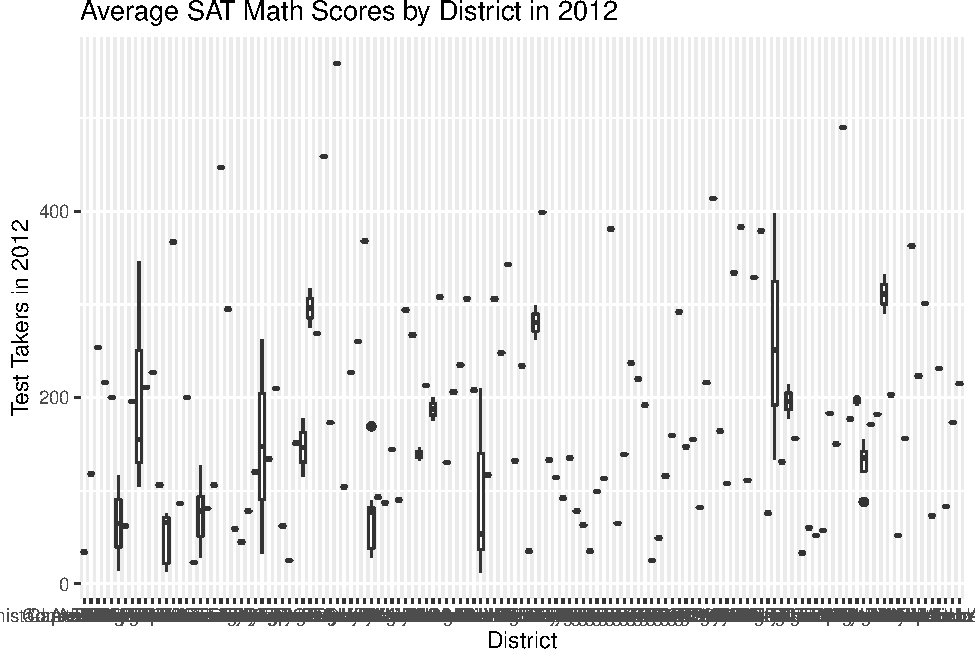
\includegraphics{code4stem_files/figure-latex/scores and titles-1.pdf}

Build sat\_scores\_gls\_lm:

\begin{Shaded}
\begin{Highlighting}[]
\NormalTok{sat_scores_gls_lm <-}\StringTok{ }\KeywordTok{lm}\NormalTok{(Test.takers..}\DecValTok{2012} \OperatorTok{~}\StringTok{ }\NormalTok{Test.takers..}\DecValTok{2013} \OperatorTok{+}\StringTok{ }\NormalTok{District }\OperatorTok{+}\StringTok{ }\NormalTok{School,}
                        \DataTypeTok{data =}\NormalTok{ sat_scores)}

\CommentTok{# Tidy the results with broom}
\KeywordTok{tidy}\NormalTok{(sat_scores_gls_lm) }\OperatorTok
\StringTok{  }\KeywordTok{head}\NormalTok{()}
\end{Highlighting}
\end{Shaded}

\begin{verbatim}
## # A tibble: 6 x 5
##   term              estimate std.error statistic p.value
##   <chr>                <dbl>     <dbl>     <dbl>   <dbl>
## 1 (Intercept)          -9.24       NaN       NaN     NaN
## 2 Test.takers..2013     1.39       NaN       NaN     NaN
## 3 DistrictAnsonia     -17.8        NaN       NaN     NaN
## 4 DistrictAvon        -75.7        NaN       NaN     NaN
## 5 DistrictBerlin      -81.6        NaN       NaN     NaN
## 6 DistrictBethel      -55.8        NaN       NaN     NaN
\end{verbatim}

Examine the results with anova

\begin{Shaded}
\begin{Highlighting}[]
\KeywordTok{anova}\NormalTok{(sat_scores_gls_lm)}
\end{Highlighting}
\end{Shaded}

\begin{verbatim}
## Warning in anova.lm(sat_scores_gls_lm): ANOVA F-tests on an essentially perfect
## fit are unreliable
\end{verbatim}

\begin{verbatim}
## Analysis of Variance Table
## 
## Response: Test.takers..2012
##                    Df  Sum Sq Mean Sq F value Pr(>F)
## Test.takers..2013   1 2144936 2144936               
## District          128   46850     366               
## School             57   31922     560               
## Residuals           0       0
\end{verbatim}

Factorial Experiment Design
2 or more factor variables are combined and crossed
All of the possible interactions between factors are considered as effect on outcome
e.g.~high/low water on high/low light

Build the boxplot for the district vs.~test taker score:

\begin{Shaded}
\begin{Highlighting}[]
\KeywordTok{ggplot}\NormalTok{(sat_scores,}
       \KeywordTok{aes}\NormalTok{(District, Test.takers..}\DecValTok{2012}\NormalTok{)) }\OperatorTok{+}\StringTok{ }
\StringTok{  }\KeywordTok{geom_boxplot}\NormalTok{()}
\end{Highlighting}
\end{Shaded}

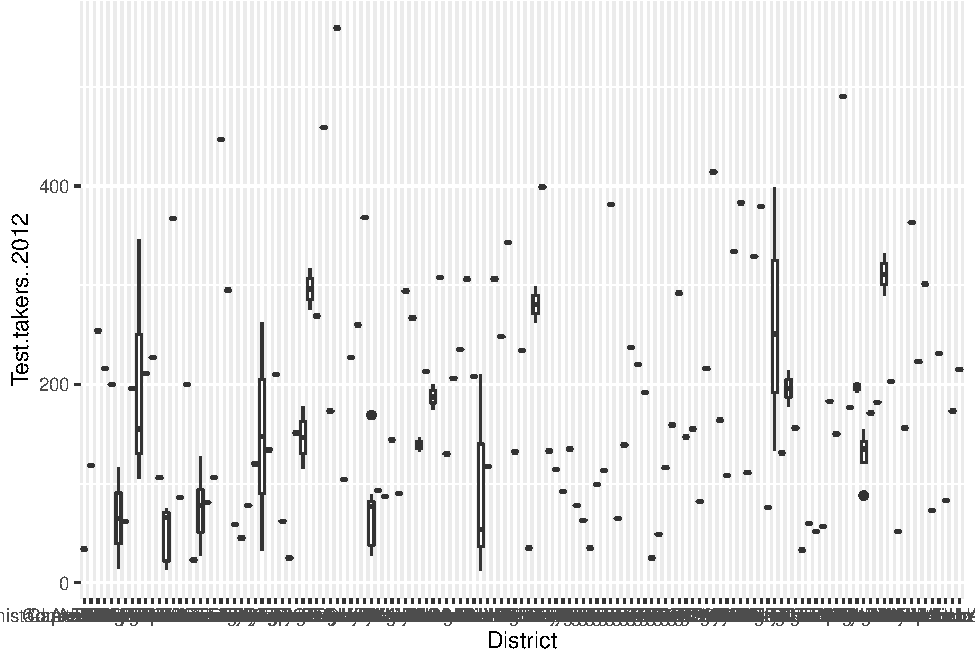
\includegraphics{code4stem_files/figure-latex/boxplot with scores-1.pdf}

Create sat\_scores\_factorial and examine the results:

\begin{Shaded}
\begin{Highlighting}[]
\NormalTok{sat_scores_factorial <-}\StringTok{ }\KeywordTok{aov}\NormalTok{(Test.takers..}\DecValTok{2012} \OperatorTok{~}\StringTok{ }\NormalTok{Test.takers..}\DecValTok{2013} \OperatorTok{*}\StringTok{ }\NormalTok{District }\OperatorTok{*}\StringTok{ }\NormalTok{School, }\DataTypeTok{data =}\NormalTok{ sat_scores)}

\KeywordTok{tidy}\NormalTok{(sat_scores_factorial) }\OperatorTok
\StringTok{  }\KeywordTok{head}\NormalTok{()}
\end{Highlighting}
\end{Shaded}

\begin{verbatim}
## # A tibble: 3 x 4
##   term                 df    sumsq   meansq
##   <chr>             <dbl>    <dbl>    <dbl>
## 1 Test.takers..2013     1 2144936. 2144936.
## 2 District            128   46850.     366.
## 3 School               57   31922.     560.
\end{verbatim}

Evaluating the sat\_scores Factorial Model

Use shapiro.test() to test the outcome:

\begin{Shaded}
\begin{Highlighting}[]
\KeywordTok{shapiro.test}\NormalTok{(sat_scores}\OperatorTok{$}\NormalTok{Test.takers..}\DecValTok{2013}\NormalTok{)}
\end{Highlighting}
\end{Shaded}

\begin{verbatim}
## 
## 	Shapiro-Wilk normality test
## 
## data:  sat_scores$Test.takers..2013
## W = 0.91495, p-value = 6.28e-09
\end{verbatim}

\hypertarget{demo-for-ab-testing}{%
\chapter{Demo for A/B testing}\label{demo-for-ab-testing}}

\begin{Shaded}
\begin{Highlighting}[]
\CommentTok{# load dependencies}
\KeywordTok{library}\NormalTok{(tidyverse)}
\KeywordTok{library}\NormalTok{(powerMediation)}
\KeywordTok{library}\NormalTok{(broom)}
\KeywordTok{library}\NormalTok{(pwr)}
\KeywordTok{library}\NormalTok{(gsDesign)}
\KeywordTok{library}\NormalTok{(powerMediation)}
\end{Highlighting}
\end{Shaded}

Read in data:

\begin{Shaded}
\begin{Highlighting}[]
\NormalTok{fileLocation <-}\StringTok{ "http://stat.columbia.edu/~rachel/datasets/nyt1.csv"}
\NormalTok{click_data <-}\StringTok{ }\KeywordTok{read.csv}\NormalTok{(}\KeywordTok{url}\NormalTok{(fileLocation))}
\end{Highlighting}
\end{Shaded}

Find oldest and most recent age:

\begin{Shaded}
\begin{Highlighting}[]
\KeywordTok{min}\NormalTok{(click_data}\OperatorTok{$}\NormalTok{Age)}
\end{Highlighting}
\end{Shaded}

\begin{verbatim}
## [1] 0
\end{verbatim}

\begin{Shaded}
\begin{Highlighting}[]
\KeywordTok{max}\NormalTok{(click_data}\OperatorTok{$}\NormalTok{Age) }
\end{Highlighting}
\end{Shaded}

\begin{verbatim}
## [1] 108
\end{verbatim}

Compute baseline conversion rates:

\begin{Shaded}
\begin{Highlighting}[]
\NormalTok{click_data }\OperatorTok
\StringTok{  }\KeywordTok{summarize}\NormalTok{(}\DataTypeTok{impression_rate =} \KeywordTok{mean}\NormalTok{(Impressions))}
\end{Highlighting}
\end{Shaded}

\begin{verbatim}
##   impression_rate
## 1        5.007316
\end{verbatim}

determine baseline for genders:

\begin{Shaded}
\begin{Highlighting}[]
\NormalTok{click_data }\OperatorTok
\StringTok{  }\KeywordTok{group_by}\NormalTok{(Gender) }\OperatorTok
\StringTok{  }\KeywordTok{summarize}\NormalTok{(}\DataTypeTok{impression_rate =} \KeywordTok{mean}\NormalTok{(Impressions))}
\end{Highlighting}
\end{Shaded}

\begin{verbatim}
## # A tibble: 2 x 2
##   Gender impression_rate
##    <int>           <dbl>
## 1      0            5.01
## 2      1            5.01
\end{verbatim}

determine baseline for clicks:

\begin{Shaded}
\begin{Highlighting}[]
\NormalTok{click_data_age<-}\StringTok{ }\NormalTok{click_data }\OperatorTok
\StringTok{  }\KeywordTok{group_by}\NormalTok{(Clicks, Age) }\OperatorTok
\StringTok{  }\KeywordTok{summarize}\NormalTok{(}\DataTypeTok{impression_rate =} \KeywordTok{mean}\NormalTok{(Impressions))}
\end{Highlighting}
\end{Shaded}

visualize baselines:

\begin{Shaded}
\begin{Highlighting}[]
\KeywordTok{ggplot}\NormalTok{(click_data_age, }\KeywordTok{aes}\NormalTok{(}\DataTypeTok{x =}\NormalTok{ Age, }\DataTypeTok{y =}\NormalTok{ impression_rate)) }\OperatorTok{+}
\StringTok{  }\KeywordTok{geom_point}\NormalTok{() }\OperatorTok{+}
\StringTok{  }\KeywordTok{geom_line}\NormalTok{() }
\end{Highlighting}
\end{Shaded}

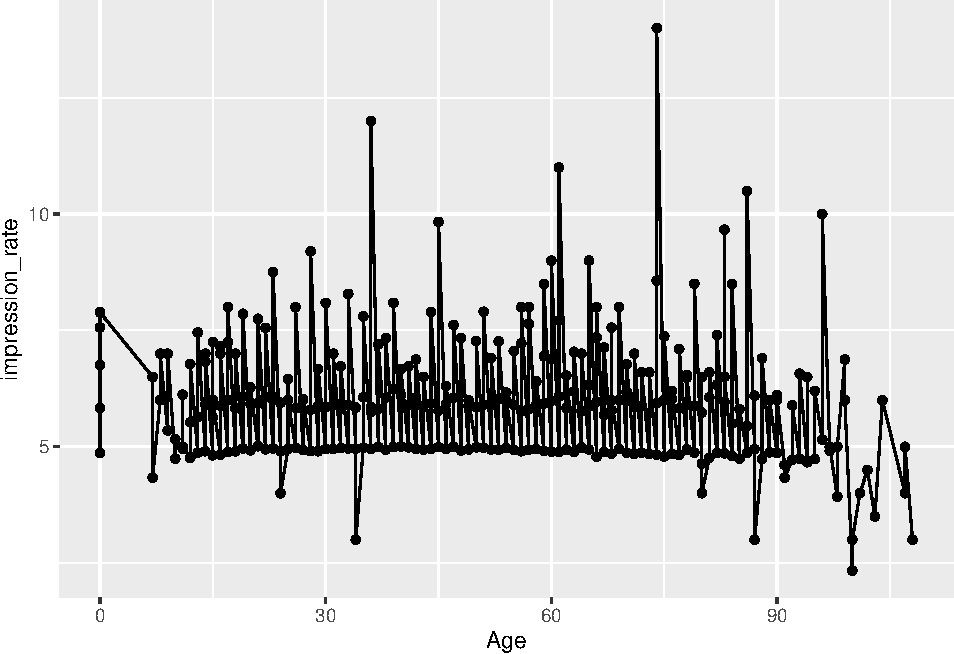
\includegraphics{code4stem_files/figure-latex/visualize baselines-1.pdf}

Experimental design, power analysis, and t-tests

run power analysis:
learn more here: help(SSizeLogisticBin)

\begin{Shaded}
\begin{Highlighting}[]
\NormalTok{total_sample_size <-}\StringTok{ }\KeywordTok{SSizeLogisticBin}\NormalTok{(}\DataTypeTok{p1 =} \FloatTok{0.2}\NormalTok{, }\CommentTok{# conversion rate for control condition}
                                      \DataTypeTok{p2 =} \FloatTok{0.3}\NormalTok{, }\CommentTok{# conversion rate for expected conversion rate for test condition: backed by previous data (e.g.30% conversion rate to get 10% boost)}
                                      \DataTypeTok{B =} \FloatTok{0.5}\NormalTok{, }\CommentTok{# most commonly used}
                                      \DataTypeTok{alpha =} \FloatTok{0.05}\NormalTok{, }\CommentTok{# most commonly used}
                                      \DataTypeTok{power =} \FloatTok{0.8}\NormalTok{) }\CommentTok{# most commonly used}
\NormalTok{total_sample_size}
\end{Highlighting}
\end{Shaded}

\begin{verbatim}
## [1] 587
\end{verbatim}

\begin{Shaded}
\begin{Highlighting}[]
\NormalTok{total_sample_size }\OperatorTok{/}\DecValTok{2} \CommentTok{# per condition}
\end{Highlighting}
\end{Shaded}

\begin{verbatim}
## [1] 293.5
\end{verbatim}

can use a ttest or linear regression for statistical tests:
lm is used when more variables are in data but similar to t-test

\begin{Shaded}
\begin{Highlighting}[]
\KeywordTok{lm}\NormalTok{(Gender }\OperatorTok{~}\StringTok{ }\NormalTok{Clicks, }\DataTypeTok{data =}\NormalTok{ click_data) }\OperatorTok
\StringTok{  }\KeywordTok{summary}\NormalTok{()}
\end{Highlighting}
\end{Shaded}

\begin{verbatim}
## 
## Call:
## lm(formula = Gender ~ Clicks, data = click_data)
## 
## Residuals:
##    Min     1Q Median     3Q    Max 
## -0.375 -0.375 -0.375  0.625  0.884 
## 
## Coefficients:
##               Estimate Std. Error t value Pr(>|t|)    
## (Intercept)  0.3750325  0.0007418  505.56   <2e-16 ***
## Clicks      -0.0863451  0.0022930  -37.66   <2e-16 ***
## ---
## Signif. codes:  0 '***' 0.001 '**' 0.01 '*' 0.05 '.' 0.1 ' ' 1
## 
## Residual standard error: 0.4813 on 458439 degrees of freedom
## Multiple R-squared:  0.003083,	Adjusted R-squared:  0.003081 
## F-statistic:  1418 on 1 and 458439 DF,  p-value: < 2.2e-16
\end{verbatim}

\begin{Shaded}
\begin{Highlighting}[]
\CommentTok{# t.test(Gender ~ Clicks, data = click_data) %>%}
\CommentTok{#  summary()}
\end{Highlighting}
\end{Shaded}

Analyzing results
Group and summarize

\begin{Shaded}
\begin{Highlighting}[]
\NormalTok{click_data_groups <-}\StringTok{ }\NormalTok{click_data }\OperatorTok
\StringTok{  }\KeywordTok{group_by}\NormalTok{(Clicks, Age) }\OperatorTok
\StringTok{  }\KeywordTok{summarize}\NormalTok{(}\DataTypeTok{impression_rate =} \KeywordTok{mean}\NormalTok{(Impressions))}
\end{Highlighting}
\end{Shaded}

Make plot of conversion rates for clicks:

\begin{Shaded}
\begin{Highlighting}[]
\KeywordTok{ggplot}\NormalTok{(click_data_groups,}
       \KeywordTok{aes}\NormalTok{(}\DataTypeTok{x =}\NormalTok{ Age,}
           \DataTypeTok{y =}\NormalTok{ impression_rate,}
           \DataTypeTok{color =}\NormalTok{ Clicks,}
           \DataTypeTok{group =}\NormalTok{ Clicks)) }\OperatorTok{+}
\StringTok{  }\KeywordTok{geom_point}\NormalTok{(}\DataTypeTok{size =} \DecValTok{3}\NormalTok{) }\OperatorTok{+}
\StringTok{  }\KeywordTok{geom_line}\NormalTok{(}\DataTypeTok{lwd =} \DecValTok{1}\NormalTok{)}
\end{Highlighting}
\end{Shaded}

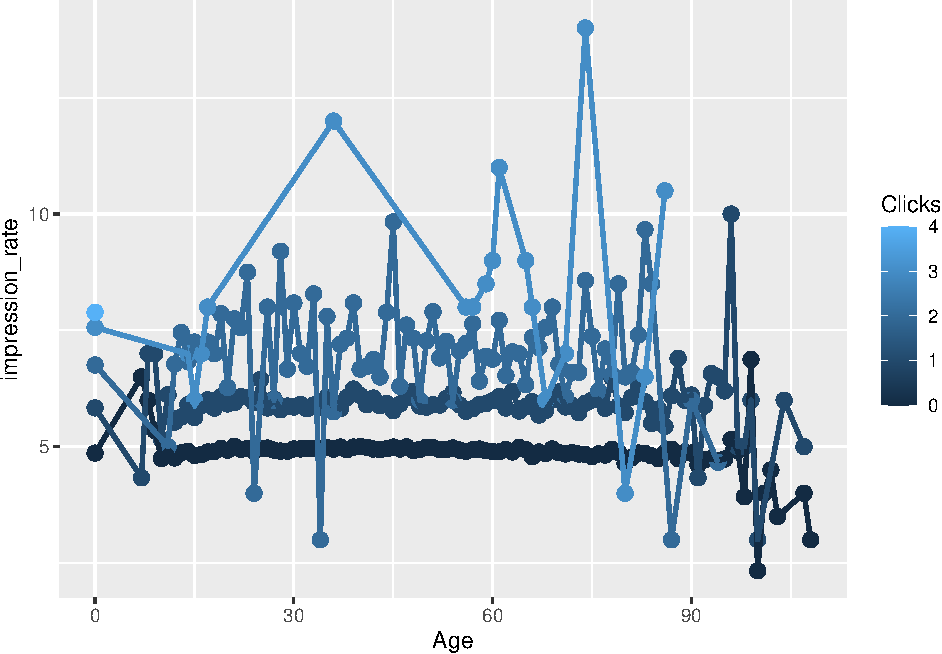
\includegraphics{code4stem_files/figure-latex/visualize clicks-1.pdf}

Make plot of conversion rates for clicks
(can add intercepts and interaction of two variables):

\begin{Shaded}
\begin{Highlighting}[]
\KeywordTok{ggplot}\NormalTok{(click_data_groups,}
       \KeywordTok{aes}\NormalTok{(}\DataTypeTok{x =}\NormalTok{ Age,}
           \DataTypeTok{y =}\NormalTok{ impression_rate,}
           \DataTypeTok{color =}\NormalTok{ Clicks,}
           \DataTypeTok{group =} \KeywordTok{interaction}\NormalTok{(Clicks, impression_rate))) }\OperatorTok{+}
\StringTok{  }\KeywordTok{geom_point}\NormalTok{(}\DataTypeTok{size =} \DecValTok{3}\NormalTok{) }\OperatorTok{+}
\StringTok{  }\KeywordTok{geom_line}\NormalTok{(}\DataTypeTok{lwd =} \DecValTok{1}\NormalTok{) }\OperatorTok{+}
\StringTok{  }\KeywordTok{geom_vline}\NormalTok{(}\DataTypeTok{xintercept =} \KeywordTok{as.numeric}\NormalTok{(}\KeywordTok{as.Date}\NormalTok{(}\StringTok{"2018-02-15"}\NormalTok{))) }
\end{Highlighting}
\end{Shaded}

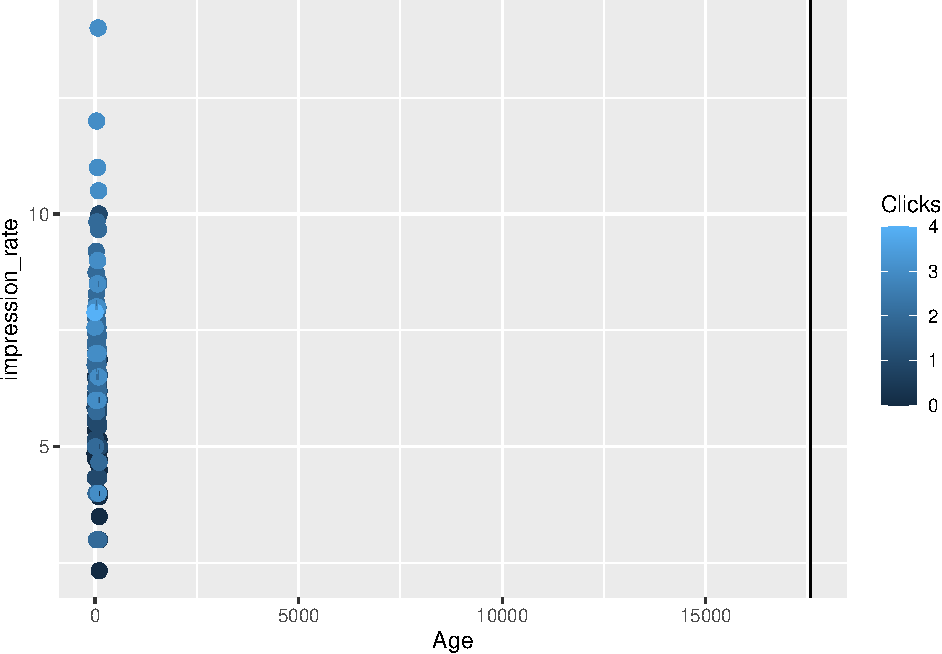
\includegraphics{code4stem_files/figure-latex/plot clicks-1.pdf}

Check for glm documentation
family can be used to express different error distributions.
?glm

Run logistic regression to analyze model outputs:

\begin{Shaded}
\begin{Highlighting}[]
\NormalTok{experiment_results <-}\StringTok{ }\KeywordTok{glm}\NormalTok{(Gender }\OperatorTok{~}\StringTok{ }\NormalTok{Clicks,}
                          \DataTypeTok{family =} \StringTok{"binomial"}\NormalTok{,}
                          \DataTypeTok{data =}\NormalTok{ click_data) }\OperatorTok
\StringTok{  }\KeywordTok{tidy}\NormalTok{()}

\NormalTok{experiment_results}
\end{Highlighting}
\end{Shaded}

\begin{verbatim}
## # A tibble: 2 x 5
##   term        estimate std.error statistic   p.value
##   <chr>          <dbl>     <dbl>     <dbl>     <dbl>
## 1 (Intercept)   -0.510   0.00319    -160.  0.       
## 2 Clicks        -0.400   0.0107      -37.3 4.10e-304
\end{verbatim}

Follow-up experimentations to test assumptions

Designing follow-up experiments since A/B testing is a continuous loops
i.e.~make new dataframes and compute various other conversion rate differences
can use spread() to reformat data

\begin{Shaded}
\begin{Highlighting}[]
\NormalTok{click_data_new_groups <-}\StringTok{ }\NormalTok{click_data }\OperatorTok
\StringTok{  }\KeywordTok{group_by}\NormalTok{(Clicks, Age) }\OperatorTok
\StringTok{  }\KeywordTok{summarize}\NormalTok{(}\DataTypeTok{impression_rate =} \KeywordTok{mean}\NormalTok{(Impressions)) }\OperatorTok\StringTok{ }
\StringTok{  }\KeywordTok{spread}\NormalTok{(Clicks, impression_rate)}
\end{Highlighting}
\end{Shaded}

Compute summary statistics:

\begin{Shaded}
\begin{Highlighting}[]
\KeywordTok{mean}\NormalTok{(click_data_new_groups}\OperatorTok{$}\NormalTok{Age, }\DataTypeTok{na.rm =} \OtherTok{TRUE}\NormalTok{)}
\end{Highlighting}
\end{Shaded}

\begin{verbatim}
## [1] 55.9802
\end{verbatim}

\begin{Shaded}
\begin{Highlighting}[]
\KeywordTok{sd}\NormalTok{(click_data_new_groups}\OperatorTok{$}\NormalTok{Age, }\DataTypeTok{na.rm =} \OtherTok{TRUE}\NormalTok{)}
\end{Highlighting}
\end{Shaded}

\begin{verbatim}
## [1] 29.4771
\end{verbatim}

Run logistic regression and power analysis
Run power analysis for logistic regression

\begin{Shaded}
\begin{Highlighting}[]
\NormalTok{total_sample_size <-}\StringTok{ }\KeywordTok{SSizeLogisticBin}\NormalTok{(}\DataTypeTok{p1 =} \FloatTok{0.49}\NormalTok{,}
                                      \DataTypeTok{p2 =} \FloatTok{0.64}\NormalTok{,}
                                      \DataTypeTok{B =} \FloatTok{0.5}\NormalTok{,}
                                      \DataTypeTok{alpha =} \FloatTok{0.05}\NormalTok{,}
                                      \DataTypeTok{power =} \FloatTok{0.8}\NormalTok{)}
\NormalTok{total_sample_size}
\end{Highlighting}
\end{Shaded}

\begin{verbatim}
## [1] 341
\end{verbatim}

View summary of data:

\begin{Shaded}
\begin{Highlighting}[]
\NormalTok{new_data <-}\StringTok{ }\NormalTok{click_data }\OperatorTok
\StringTok{  }\KeywordTok{group_by}\NormalTok{(Clicks) }\OperatorTok
\StringTok{  }\KeywordTok{summarize}\NormalTok{(}\DataTypeTok{impression_rate =} \KeywordTok{mean}\NormalTok{(Impressions)}\OperatorTok{/}\DecValTok{10}\NormalTok{)}

\CommentTok{# Run logistic regression to analyze model outputs}
\NormalTok{followup_experiment_sep_results <-}\StringTok{ }\KeywordTok{glm}\NormalTok{(impression_rate }\OperatorTok{~}\StringTok{ }\NormalTok{Clicks,}
                                       \DataTypeTok{family =} \StringTok{"binomial"}\NormalTok{,}
                                       \DataTypeTok{data =}\NormalTok{ new_data) }\OperatorTok
\StringTok{  }\KeywordTok{tidy}\NormalTok{()}
\end{Highlighting}
\end{Shaded}

\begin{verbatim}
## Warning in eval(family$initialize): non-integer #successes in a binomial glm!
\end{verbatim}

\begin{Shaded}
\begin{Highlighting}[]
\NormalTok{followup_experiment_sep_results}
\end{Highlighting}
\end{Shaded}

\begin{verbatim}
## # A tibble: 2 x 5
##   term        estimate std.error statistic p.value
##   <chr>          <dbl>     <dbl>     <dbl>   <dbl>
## 1 (Intercept)  0.00899     1.59    0.00566   0.995
## 2 Clicks       0.361       0.710   0.509     0.611
\end{verbatim}

Specifics of A/B Testing= use of experimental design to compare 2 or more variants of a design
Test Types: A/B, A/A, A/B/N test conditions
Assumptions to test: within group vs.~between group experiments

e.g.~plotting A/A data
Compute conversion rates for A/A experiment:

\begin{Shaded}
\begin{Highlighting}[]
\NormalTok{click_data_sum <-}\StringTok{ }\NormalTok{click_data }\OperatorTok
\StringTok{  }\KeywordTok{group_by}\NormalTok{(Signed_In) }\OperatorTok
\StringTok{  }\KeywordTok{summarize}\NormalTok{(}\DataTypeTok{impression_rate =} \KeywordTok{mean}\NormalTok{(Impressions)}\OperatorTok{/}\DecValTok{10}\NormalTok{)}
\NormalTok{click_data_sum}
\end{Highlighting}
\end{Shaded}

\begin{verbatim}
## # A tibble: 2 x 2
##   Signed_In impression_rate
##       <int>           <dbl>
## 1         0           0.500
## 2         1           0.501
\end{verbatim}

Plot conversion rates for two conditions:

\begin{Shaded}
\begin{Highlighting}[]
\KeywordTok{ggplot}\NormalTok{(click_data_sum,}
       \KeywordTok{aes}\NormalTok{(}\DataTypeTok{x =}\NormalTok{ Signed_In, }\DataTypeTok{y =}\NormalTok{ impression_rate)) }\OperatorTok{+}
\StringTok{  }\KeywordTok{geom_bar}\NormalTok{(}\DataTypeTok{stat =} \StringTok{"identity"}\NormalTok{)  }
\end{Highlighting}
\end{Shaded}

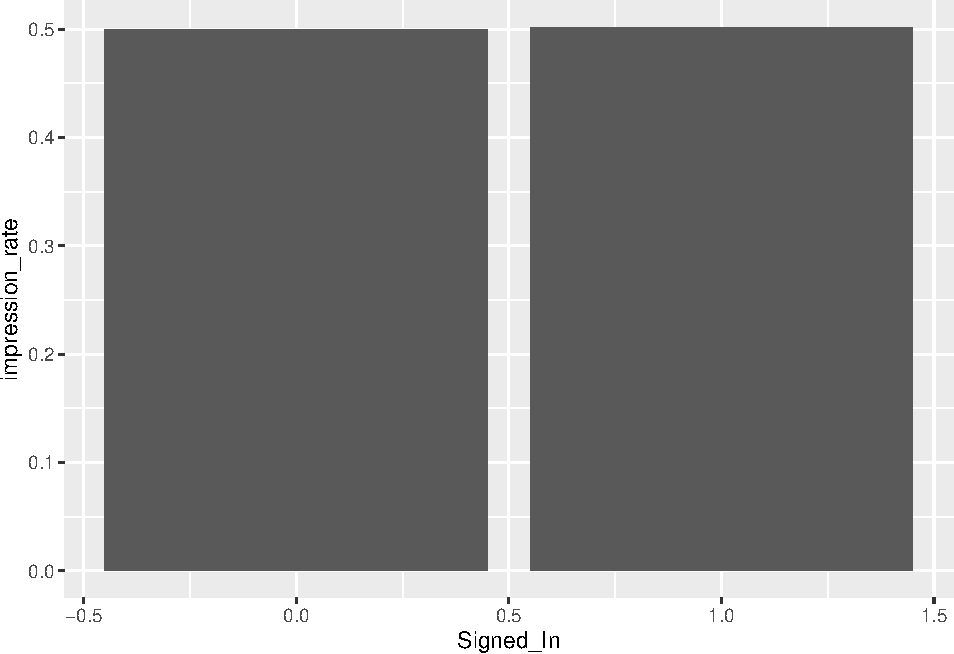
\includegraphics{code4stem_files/figure-latex/plot conversion rates-1.pdf}

\begin{Shaded}
\begin{Highlighting}[]
\CommentTok{#Based on these bar plots the two A conditions look very similar. That's good!}
\end{Highlighting}
\end{Shaded}

Run logistic regression to analyze model outputs:

\begin{Shaded}
\begin{Highlighting}[]
\NormalTok{aa_experiment_results <-}\StringTok{ }\KeywordTok{glm}\NormalTok{(Signed_In }\OperatorTok{~}\StringTok{ }\NormalTok{impression_rate,}
                             \DataTypeTok{family =} \StringTok{"binomial"}\NormalTok{,}
                             \DataTypeTok{data =}\NormalTok{ click_data_sum) }\OperatorTok
\StringTok{  }\KeywordTok{tidy}\NormalTok{()}
\NormalTok{aa_experiment_results}
\end{Highlighting}
\end{Shaded}

\begin{verbatim}
## # A tibble: 2 x 5
##   term            estimate  std.error statistic p.value
##   <chr>              <dbl>      <dbl>     <dbl>   <dbl>
## 1 (Intercept)      -21589.  51475133. -0.000419    1.00
## 2 impression_rate   43135. 102844880.  0.000419    1.00
\end{verbatim}

Confounding variables: element that can affect the truth of A/B exp
change one element at a time to know the change you are testing
Need to also consider the side effects
procedures are the same as above

Power analysis requires 3 variables: power (1-beta) , significance level (alpha or p-value), effect size
as power goes up, so does the of data points needed
as significance level goes up (i.e.~more significant), so do of data points needed
as effect sizw increase, of data points decrease
ttest (linear regression) can be used for continuous dependent variable (e.g.~time spent on a website)

\begin{Shaded}
\begin{Highlighting}[]
\KeywordTok{pwr.t.test}\NormalTok{(}\DataTypeTok{power =} \FloatTok{0.8}\NormalTok{,}
           \DataTypeTok{sig.level =} \FloatTok{0.05}\NormalTok{,}
           \DataTypeTok{d =} \FloatTok{0.6}\NormalTok{)  }\CommentTok{# d = effect size }
\end{Highlighting}
\end{Shaded}

\begin{verbatim}
## 
##      Two-sample t test power calculation 
## 
##               n = 44.58577
##               d = 0.6
##       sig.level = 0.05
##           power = 0.8
##     alternative = two.sided
## 
## NOTE: n is number in *each* group
\end{verbatim}

\begin{Shaded}
\begin{Highlighting}[]
\KeywordTok{pwr.t.test}\NormalTok{(}\DataTypeTok{power =} \FloatTok{0.8}\NormalTok{,}
           \DataTypeTok{sig.level =} \FloatTok{0.05}\NormalTok{,}
           \DataTypeTok{d =} \FloatTok{0.2}\NormalTok{) }\CommentTok{#(see more on experimental design)}
\end{Highlighting}
\end{Shaded}

\begin{verbatim}
## 
##      Two-sample t test power calculation 
## 
##               n = 393.4057
##               d = 0.2
##       sig.level = 0.05
##           power = 0.8
##     alternative = two.sided
## 
## NOTE: n is number in *each* group
\end{verbatim}

Load package to run power analysis: library(powerMediation)

logistic regression can be used for categorical dependent variable (e.g.~click or not click)
Run power analysis for logistic regression

\begin{Shaded}
\begin{Highlighting}[]
\NormalTok{total_sample_size <-}\StringTok{ }\KeywordTok{SSizeLogisticBin}\NormalTok{(}\DataTypeTok{p1 =} \FloatTok{0.17}\NormalTok{, }\CommentTok{# assuming a control value of 17%}
                                      \DataTypeTok{p2 =} \FloatTok{0.27}\NormalTok{, }\CommentTok{# assuming 10% increase in the test condition}
                                      \DataTypeTok{B =} \FloatTok{0.5}\NormalTok{,}
                                      \DataTypeTok{alpha =} \FloatTok{0.05}\NormalTok{,}
                                      \DataTypeTok{power =} \FloatTok{0.8}\NormalTok{)}
\NormalTok{total_sample_size}
\end{Highlighting}
\end{Shaded}

\begin{verbatim}
## [1] 537
\end{verbatim}

Stopping rules and sequential analysis
procedures that allow interim analyses in pre-defined points = sequential analysis

\begin{Shaded}
\begin{Highlighting}[]
\NormalTok{seq_analysis <-}\StringTok{ }\KeywordTok{gsDesign}\NormalTok{(}\DataTypeTok{k=}\DecValTok{4}\NormalTok{, }\CommentTok{# number of times you want to look at the data}
                         \DataTypeTok{test.type =} \DecValTok{1}\NormalTok{,}
                         \DataTypeTok{alpha =} \FloatTok{0.05}\NormalTok{,}
                         \DataTypeTok{beta =} \FloatTok{0.2}\NormalTok{, }\CommentTok{# power = 1-beta so power is 0.8}
                         \DataTypeTok{sfu =} \StringTok{"Pocock"}\NormalTok{) }\CommentTok{# spending function to figure out how to update p-values}
\NormalTok{seq_analysis}
\end{Highlighting}
\end{Shaded}

\begin{verbatim}
## One-sided group sequential design with
## 80 % power and 5 % Type I Error.
##            Sample
##             Size 
##   Analysis Ratio*  Z   Nominal p  Spend
##          1  0.306 2.07    0.0193 0.0193
##          2  0.612 2.07    0.0193 0.0132
##          3  0.918 2.07    0.0193 0.0098
##          4  1.224 2.07    0.0193 0.0077
##      Total                       0.0500 
## 
## ++ alpha spending:
##  Pocock boundary.
## * Sample size ratio compared to fixed design with no interim
## 
## Boundary crossing probabilities and expected sample size
## assume any cross stops the trial
## 
## Upper boundary (power or Type I Error)
##           Analysis
##    Theta      1      2      3      4 Total   E{N}
##   0.0000 0.0193 0.0132 0.0098 0.0077  0.05 1.1952
##   2.4865 0.2445 0.2455 0.1845 0.1255  0.80 0.7929
\end{verbatim}

\begin{Shaded}
\begin{Highlighting}[]
\NormalTok{max_n <-}\StringTok{ }\DecValTok{1000}
\NormalTok{max_n_per_group <-}\StringTok{ }\NormalTok{max_n }\OperatorTok{/}\StringTok{ }\DecValTok{2}
\NormalTok{stopping_points <-}\StringTok{ }\NormalTok{max_n_per_group }\OperatorTok{*}\StringTok{ }\NormalTok{seq_analysis}\OperatorTok{$}\NormalTok{timing}
\NormalTok{stopping_points}
\end{Highlighting}
\end{Shaded}

\begin{verbatim}
## [1] 125 250 375 500
\end{verbatim}

Run sequential analysis:

\begin{Shaded}
\begin{Highlighting}[]
\NormalTok{seq_analysis_3looks <-}\StringTok{ }\KeywordTok{gsDesign}\NormalTok{(}\DataTypeTok{k =} \DecValTok{3}\NormalTok{,}
                                \DataTypeTok{test.type =} \DecValTok{1}\NormalTok{,}
                                \DataTypeTok{alpha =} \FloatTok{0.05}\NormalTok{,}
                                \DataTypeTok{beta =} \FloatTok{0.2}\NormalTok{,}
                                \DataTypeTok{sfu =} \StringTok{"Pocock"}\NormalTok{)}
\NormalTok{seq_analysis_3looks}
\end{Highlighting}
\end{Shaded}

\begin{verbatim}
## One-sided group sequential design with
## 80 % power and 5 % Type I Error.
##            Sample
##             Size 
##   Analysis Ratio*  Z   Nominal p  Spend
##          1  0.394 1.99    0.0232 0.0232
##          2  0.789 1.99    0.0232 0.0155
##          3  1.183 1.99    0.0232 0.0113
##      Total                       0.0500 
## 
## ++ alpha spending:
##  Pocock boundary.
## * Sample size ratio compared to fixed design with no interim
## 
## Boundary crossing probabilities and expected sample size
## assume any cross stops the trial
## 
## Upper boundary (power or Type I Error)
##           Analysis
##    Theta      1      2      3 Total   E{N}
##   0.0000 0.0232 0.0155 0.0113  0.05 1.1591
##   2.4865 0.3334 0.2875 0.1791  0.80 0.8070
\end{verbatim}

Fill in max number of points and compute points per group and find stopping points

\begin{Shaded}
\begin{Highlighting}[]
\NormalTok{max_n <-}\StringTok{ }\DecValTok{3000}
\NormalTok{max_n_per_group <-}\StringTok{ }\NormalTok{max_n }\OperatorTok{/}\StringTok{ }\DecValTok{2}
\NormalTok{stopping_points =}\StringTok{ }\NormalTok{max_n_per_group }\OperatorTok{*}\StringTok{ }\NormalTok{seq_analysis_3looks}\OperatorTok{$}\NormalTok{timing}
\NormalTok{stopping_points}
\end{Highlighting}
\end{Shaded}

\begin{verbatim}
## [1]  500 1000 1500
\end{verbatim}

Multivariate testing (i.e.~more than one independent variable in the experiment)

Compute summary values for four conditions

\begin{Shaded}
\begin{Highlighting}[]
\NormalTok{new_click_data <-}\StringTok{ }\NormalTok{click_data }\OperatorTok
\StringTok{  }\KeywordTok{group_by}\NormalTok{(Age, Gender, Clicks) }\OperatorTok
\StringTok{  }\KeywordTok{summarize}\NormalTok{(}\DataTypeTok{impression_mean =} \KeywordTok{mean}\NormalTok{(Impressions))}

\CommentTok{# Plot summary values for four conditions}
\KeywordTok{ggplot}\NormalTok{(new_click_data,}
       \KeywordTok{aes}\NormalTok{(}\DataTypeTok{x =}\NormalTok{ Gender,}
           \DataTypeTok{y =}\NormalTok{ impression_mean,}
           \DataTypeTok{color =}\NormalTok{ Clicks,}
           \DataTypeTok{fill =}\NormalTok{ Age)) }\OperatorTok{+}
\StringTok{  }\KeywordTok{geom_bar}\NormalTok{(}\DataTypeTok{stat =} \StringTok{"identity"}\NormalTok{, }\DataTypeTok{position =} \StringTok{"dodge"}\NormalTok{)}
\end{Highlighting}
\end{Shaded}

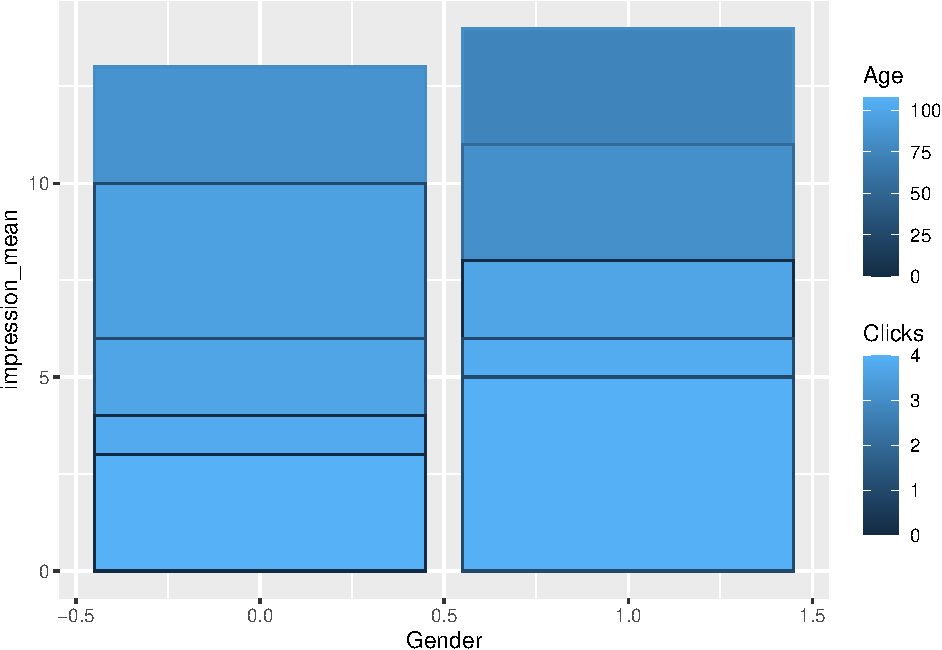
\includegraphics{code4stem_files/figure-latex/use broom to visualize clicks-1.pdf}

\begin{Shaded}
\begin{Highlighting}[]
\NormalTok{multivar_results <-}\StringTok{ }\KeywordTok{lm}\NormalTok{(Age }\OperatorTok{~}\StringTok{ }\NormalTok{Gender }\OperatorTok{*}\StringTok{ }\NormalTok{Clicks, }\DataTypeTok{data =}\NormalTok{ click_data) }\OperatorTok
\StringTok{  }\KeywordTok{tidy}\NormalTok{()}

\NormalTok{multivar_results}\OperatorTok{$}\NormalTok{p.value }\CommentTok{#none are significant}
\end{Highlighting}
\end{Shaded}

\begin{verbatim}
## [1]  0.000000e+00  0.000000e+00  0.000000e+00 3.569988e-236
\end{verbatim}

\begin{Shaded}
\begin{Highlighting}[]
\NormalTok{multivar_results}
\end{Highlighting}
\end{Shaded}

\begin{verbatim}
## # A tibble: 4 x 5
##   term          estimate std.error statistic   p.value
##   <chr>            <dbl>     <dbl>     <dbl>     <dbl>
## 1 (Intercept)      23.4     0.0427     549.  0.       
## 2 Gender           17.2     0.0699     246.  0.       
## 3 Clicks           -5.00    0.123      -40.8 0.       
## 4 Gender:Clicks     7.72    0.235       32.8 3.57e-236
\end{verbatim}

Organize variables and run logistic regression:

\begin{Shaded}
\begin{Highlighting}[]
\NormalTok{new_click_data_results <-}\StringTok{ }\NormalTok{click_data }\OperatorTok
\StringTok{  }\KeywordTok{mutate}\NormalTok{(}\DataTypeTok{gender =} \KeywordTok{factor}\NormalTok{(Gender,}
                           \DataTypeTok{levels =} \KeywordTok{c}\NormalTok{(}\StringTok{"0"}\NormalTok{, }\StringTok{"1"}\NormalTok{))) }\OperatorTok
\StringTok{  }\KeywordTok{mutate}\NormalTok{(}\DataTypeTok{clicks =} \KeywordTok{factor}\NormalTok{(Clicks,}
                           \DataTypeTok{levels =} \KeywordTok{c}\NormalTok{(}\StringTok{"1"}\NormalTok{, }\StringTok{"0"}\NormalTok{))) }\OperatorTok
\StringTok{  }\KeywordTok{glm}\NormalTok{(gender }\OperatorTok{~}\StringTok{ }\NormalTok{gender }\OperatorTok{*}\StringTok{ }\NormalTok{clicks,}
      \DataTypeTok{family =} \StringTok{"binomial"}\NormalTok{,}
      \DataTypeTok{data =}\NormalTok{ .) }\OperatorTok
\StringTok{  }\KeywordTok{tidy}\NormalTok{()}
\end{Highlighting}
\end{Shaded}

\begin{verbatim}
## Warning in model.matrix.default(...): the response appeared on the right-hand
## side and was dropped
\end{verbatim}

\begin{verbatim}
## Warning in model.matrix.default(...): problem with term 1 in model.matrix: no
## columns are assigned
\end{verbatim}

\begin{Shaded}
\begin{Highlighting}[]
\NormalTok{new_click_data_results}
\end{Highlighting}
\end{Shaded}

\begin{verbatim}
## # A tibble: 3 x 5
##   term            estimate std.error statistic p.value
##   <chr>              <dbl>     <dbl>     <dbl>   <dbl>
## 1 (Intercept)       -0.894    0.0114   -78.5     0    
## 2 clicks0          -21.7     94.2       -0.230   0.818
## 3 gender1:clicks0   45.1    154.         0.293   0.769
\end{verbatim}

\hypertarget{r-for-reporting}{%
\chapter{R for Reporting}\label{r-for-reporting}}

Possible ways to report your findings include e-mailing figures and tables around with some explanatory text or creating reports in Word, LaTeX or HTML.

R code used to produce the figures and tables is typically not part of these documents. So in case the data changes, e.g., if new data becomes available, the code needs to be re-run and all the figures and tables updated. This can be rather cumbersome. If code and reporting are not in the same place, it can also be a bit of a hassle to reconstruct the details of the analysis carried out to produce the results.

To enable reproducible data analysis and research, the idea of dynamic reporting is that data, code and results are all in one place. This can for example be a R Markdown document like this one. Generating the report automatically executes the analysis code and includes the results in the report.

\hypertarget{usage-demonstrations}{%
\section{Usage demonstrations}\label{usage-demonstrations}}

\hypertarget{inline-code}{%
\subsection{Inline code}\label{inline-code}}

Simple pieces of code can be included inline. This can be handy to, e.g., include the number of observations in your data set dynamically. The \emph{cars} data set, often used to illustrate the linear model, has 50 observations.

\hypertarget{code-chunks}{%
\subsection{Code chunks}\label{code-chunks}}

You can include typical output like a summary of your data set and a summary of a linear model through code chunks.

\begin{Shaded}
\begin{Highlighting}[]
\KeywordTok{summary}\NormalTok{(cars)}
\end{Highlighting}
\end{Shaded}

\begin{verbatim}
##      speed           dist       
##  Min.   : 4.0   Min.   :  2.00  
##  1st Qu.:12.0   1st Qu.: 26.00  
##  Median :15.0   Median : 36.00  
##  Mean   :15.4   Mean   : 42.98  
##  3rd Qu.:19.0   3rd Qu.: 56.00  
##  Max.   :25.0   Max.   :120.00
\end{verbatim}

\begin{Shaded}
\begin{Highlighting}[]
\NormalTok{m <-}\StringTok{ }\KeywordTok{lm}\NormalTok{(dist }\OperatorTok{~}\StringTok{ }\NormalTok{speed, }\DataTypeTok{data =}\NormalTok{ cars)}
\KeywordTok{summary}\NormalTok{(m)}
\end{Highlighting}
\end{Shaded}

\begin{verbatim}
## 
## Call:
## lm(formula = dist ~ speed, data = cars)
## 
## Residuals:
##     Min      1Q  Median      3Q     Max 
## -29.069  -9.525  -2.272   9.215  43.201 
## 
## Coefficients:
##             Estimate Std. Error t value Pr(>|t|)    
## (Intercept) -17.5791     6.7584  -2.601   0.0123 *  
## speed         3.9324     0.4155   9.464 1.49e-12 ***
## ---
## Signif. codes:  0 '***' 0.001 '**' 0.01 '*' 0.05 '.' 0.1 ' ' 1
## 
## Residual standard error: 15.38 on 48 degrees of freedom
## Multiple R-squared:  0.6511,	Adjusted R-squared:  0.6438 
## F-statistic: 89.57 on 1 and 48 DF,  p-value: 1.49e-12
\end{verbatim}

\hypertarget{include-tables}{%
\subsubsection{Include tables}\label{include-tables}}

The estimated coefficients, as well as their standard errors, t-values and p-values can also be included in the form of a table, for example through \textbf{knitr}'s \texttt{kable} function.

\begin{Shaded}
\begin{Highlighting}[]
\KeywordTok{library}\NormalTok{(}\StringTok{"knitr"}\NormalTok{)}
\KeywordTok{kable}\NormalTok{(}\KeywordTok{summary}\NormalTok{(m)}\OperatorTok{$}\NormalTok{coef, }\DataTypeTok{digits =} \DecValTok{2}\NormalTok{)}
\end{Highlighting}
\end{Shaded}

\begin{tabular}{l|r|r|r|r}
\hline
  & Estimate & Std. Error & t value & Pr(>|t|)\\
\hline
(Intercept) & -17.58 & 6.76 & -2.60 & 0.01\\
\hline
speed & 3.93 & 0.42 & 9.46 & 0.00\\
\hline
\end{tabular}

\hypertarget{include-figures}{%
\subsubsection{Include figures}\label{include-figures}}

The \textbf{trackeR} package provides infrastructure for running and cycling data in \textbf{R} and is used here to illustrate how figures can be included.

\begin{Shaded}
\begin{Highlighting}[]
\CommentTok{## install.packages("devtools")}
\CommentTok{## devtools::install_github("hfrick/trackeR")}
\KeywordTok{library}\NormalTok{(}\StringTok{"trackeR"}\NormalTok{) }
\KeywordTok{data}\NormalTok{(}\StringTok{"runs"}\NormalTok{, }\DataTypeTok{package =} \StringTok{"trackeR"}\NormalTok{)}
\end{Highlighting}
\end{Shaded}

A plot of how heart rate and pace evolve over time in 10 training sessions looks like this

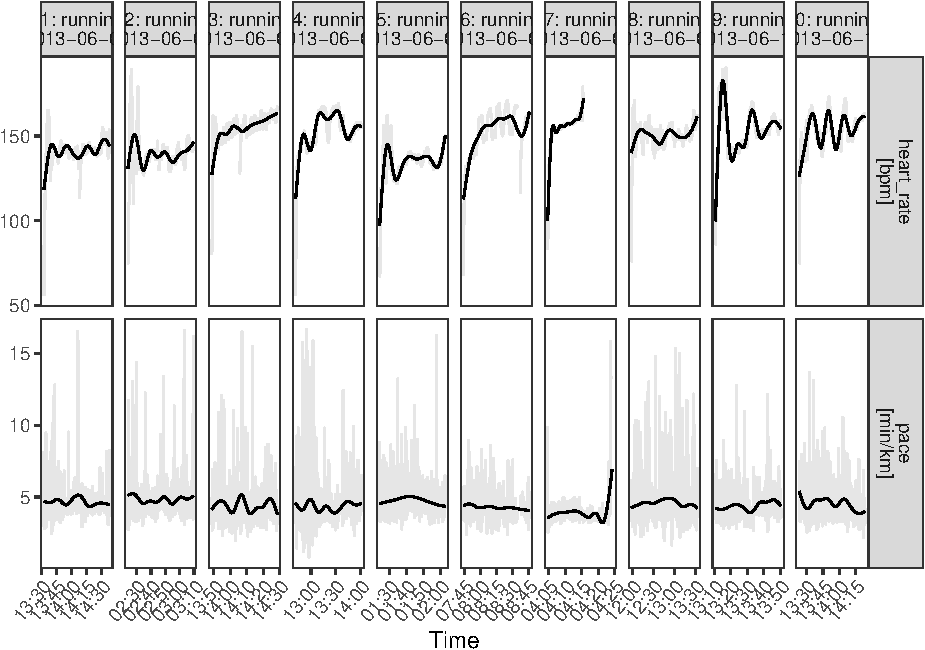
\includegraphics{code4stem_files/figure-latex/unnamed-chunk-4-1.pdf}

but the plot looks better with a wider plotting window.

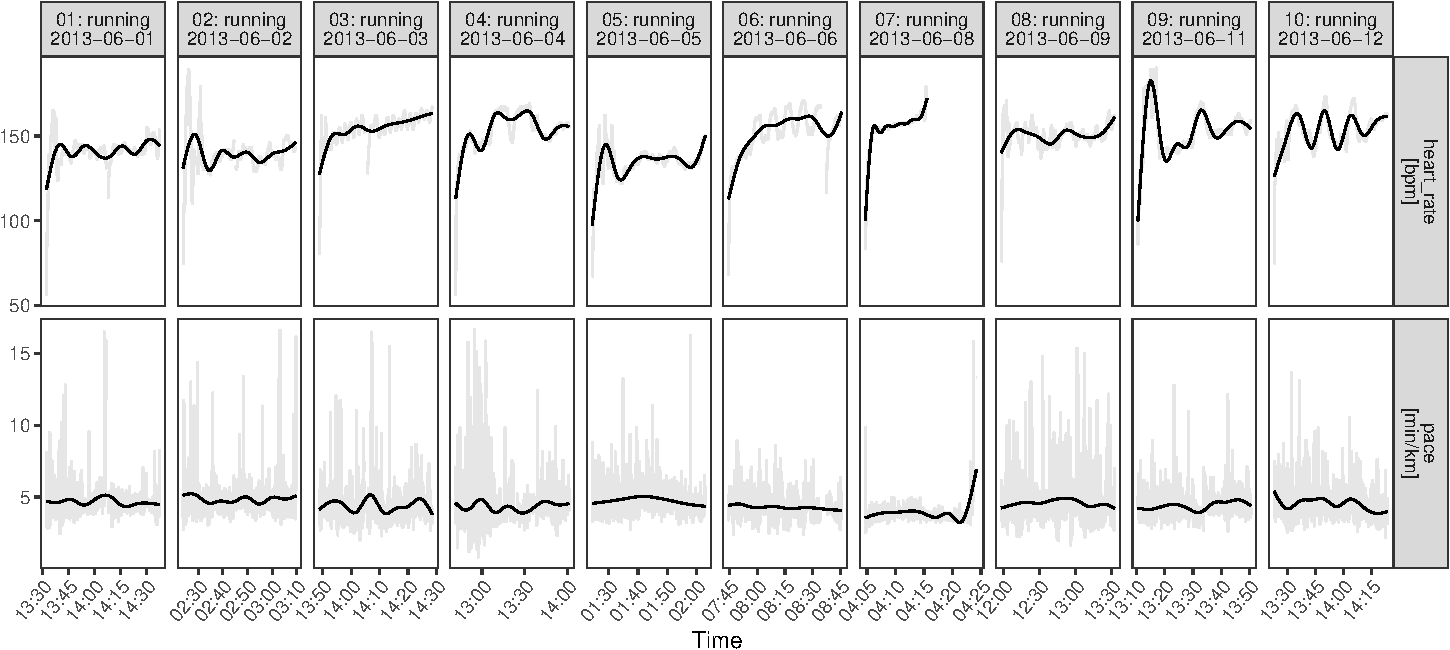
\includegraphics{code4stem_files/figure-latex/unnamed-chunk-5-1.pdf}

\hypertarget{resources}{%
\section{Resources}\label{resources}}

\begin{itemize}
\tightlist
\item
  \href{http://daringfireball.net/projects/markdown/}{Markdown main page}
\item
  \href{http://rmarkdown.rstudio.com/}{R Markdown}
\item
  \href{http://kbroman.org/knitr_knutshell/}{knitr in a nutshell} tutorial by Karl Broman
\end{itemize}

\begin{center}\rule{0.5\linewidth}{0.5pt}\end{center}

\hypertarget{beginner-resources-by-topic}{%
\section{Beginner Resources by Topic}\label{beginner-resources-by-topic}}

\begin{center}\rule{0.5\linewidth}{0.5pt}\end{center}

\hypertarget{getting-set-up-with-r-rstudio}{%
\subsection{Getting Set-Up with R \& RStudio}\label{getting-set-up-with-r-rstudio}}

\begin{itemize}
\tightlist
\item
  \textbf{Download \& Install R:}

  \begin{itemize}
  \tightlist
  \item
    \url{https://cran.r-project.org}
  \item
    For Mac: click on \textbf{Download R for (Mac) OS X}, look at the top link under \textbf{Files}, which at time of writing is \textbf{R-3.2.4.pkg}, and download this if compatible with your current version mac OS (Mavericks 10.9 or higher). Otherwise download the version beneath it which is compatible for older mac OS versions. Then install the downloaded software.
  \item
    For Windows: click on \textbf{Download R for Windows}, then click on the link \textbf{install R for the first time}, and download from the large link at the top of the page which at time of writing is \textbf{Download R 3.2.4 for Windows}. Then install the downloaded software.
  \end{itemize}
\item
  \textbf{Download \& Install RStudio:}

  \begin{itemize}
  \tightlist
  \item
    \url{https://www.rstudio.com/products/rstudio/download/}
  \item
    For Mac: under the \textbf{Installers for Supported Platforms} heading click the link with \textbf{Mac OS X} in it. Install the downloaded software.
  \item
    For Windows: under the \textbf{Installers for Supported Platforms} heading click the link with \textbf{Windows Vista} in it. Install the downloaded software.
  \end{itemize}
\item
  \textbf{Exercises in R: swirl (HIGHLY RECOMMENDED):}

  \begin{itemize}
  \tightlist
  \item
    \url{http://swirlstats.com/students.html}
  \end{itemize}
\item
  \textbf{Data Prep}:

  \begin{itemize}
  \tightlist
  \item
    Intro to dplyr: \url{https://cran.rstudio.com/web/packages/dplyr/vignettes/introduction.html}
  \item
    Data Manipulation (detailed): \url{http://www.sr.bham.ac.uk/~ajrs/R/index.html}
  \item
    Aggregation and Restructing Data (base \& reshape): \url{http://www.r-statistics.com/2012/01/aggregation-and-restructuring-data-from-r-in-action/}
  \end{itemize}
\item
  \textbf{Data Types intro}: Vectors, Matrices, Arrays, Data Frames, Lists, Factors: \url{http://www.statmethods.net/input/datatypes.html}
\item
  \textbf{Using Dates and Times}: \url{http://www.cyclismo.org/tutorial/R/time.html}
\item
  \textbf{Text Data and Character Strings}: \url{http://gastonsanchez.com/Handling_and_Processing_Strings_in_R.pdf}
\item
  \textbf{Data Mining}: \url{http://www.rdatamining.com}
\end{itemize}

\begin{center}\rule{0.5\linewidth}{0.5pt}\end{center}

\begin{itemize}
\tightlist
\item
  \textbf{Data Viz}:

  \begin{itemize}
  \tightlist
  \item
    ggplot2 Cheat Sheet (RECOMMENDED): \url{http://zevross.com/blog/2014/08/04/beautiful-plotting-in-r-a-ggplot2-cheatsheet-3/}
  \item
    ggplot2 theoretical tutorial (detailed but RECOMMENDED): \url{http://www.ling.upenn.edu/~joseff/avml2012/}
  \item
    Examples of base R, ggplot2, and rCharts: \url{http://patilv.com/Replication-of-few-graphs-charts-in-base-R-ggplot2-and-rCharts-part-1-base-R/}
  \item
    Intro to ggplot2: \url{http://heather.cs.ucdavis.edu/~matloff/GGPlot2/GGPlot2Intro.pdf}
  \end{itemize}
\item
  \textbf{Interactive Visualisations}:

  \begin{itemize}
  \tightlist
  \item
    Interactive graphics (rCharts, jQuery): \url{http://www.computerworld.com/article/2473365/business-intelligence/business-intelligence-106897-how-to-turn-csv-data-into-interactive-visualizations-with-r-and-rchart.html}
  \end{itemize}
\end{itemize}

\begin{center}\rule{0.5\linewidth}{0.5pt}\end{center}

\begin{itemize}
\tightlist
\item
  \textbf{Statistics}:

  \begin{itemize}
  \tightlist
  \item
    Detailed Statistics Primer: \url{http://health.adelaide.edu.au/psychology/ccs/docs/lsr/lsr-0.3.pdf}
  \item
    Beginner guide to statistical topics in R: \url{http://www.cyclismo.org/tutorial/R/}
  \end{itemize}
\item
  \textbf{Linear Models}: \url{http://data.princeton.edu/R/gettingStarted.html}
\item
  \textbf{Time Series Analysis}: \url{https://www.otexts.org/fpp/resources}
\item
  \textbf{Little Book of R series}:

  \begin{itemize}
  \tightlist
  \item
    Time Series: \url{http://a-little-book-of-r-for-time-series.readthedocs.org/en/latest/}
  \item
    Biomedical Statistics: \url{http://a-little-book-of-r-for-biomedical-statistics.readthedocs.org/en/latest/}
  \item
    Multivariate Statistics: \url{http://little-book-of-r-for-multivariate-analysis.readthedocs.org/en/latest/}
  \end{itemize}
\end{itemize}

\begin{center}\rule{0.5\linewidth}{0.5pt}\end{center}

\begin{itemize}
\tightlist
\item
  \textbf{RStudio Cheat Sheets}:

  \begin{itemize}
  \tightlist
  \item
    RStudio IDE: \url{http://www.rstudio.com/wp-content/uploads/2016/01/rstudio-IDE-cheatsheet.pdf}
  \item
    Data Wrangling (dplyr \& tidyr): \url{https://www.rstudio.com/wp-content/uploads/2015/02/data-wrangling-cheatsheet.pdf}
  \item
    Data Viz (ggplot2): \url{https://www.rstudio.com/wp-content/uploads/2015/03/ggplot2-cheatsheet.pdf}
  \item
    Reproducible Reports (markdown): \url{https://www.rstudio.com/wp-content/uploads/2015/02/rmarkdown-cheatsheet.pdf}
  \item
    Interactive Web Apps (shiny): \url{https://www.rstudio.com/wp-content/uploads/2015/02/shiny-cheatsheet.pdf}
  \end{itemize}
\end{itemize}

\begin{center}\rule{0.5\linewidth}{0.5pt}\end{center}

\hypertarget{specialist-topics}{%
\subsection{Specialist Topics}\label{specialist-topics}}

\begin{itemize}
\tightlist
\item
  \textbf{Google Analytics}: \url{http://online-behavior.com/analytics/r}
\item
  \textbf{Spatial Cheat Sheet}: \url{http://www.maths.lancs.ac.uk/~rowlings/Teaching/UseR2012/cheatsheet.html}
\item
  \textbf{Translating between R and SQL}: \url{http://www.burns-stat.com/translating-r-sql-basics/}
\item
  \textbf{Google's R style guide}: \url{https://google.github.io/styleguide/Rguide.xml}
\end{itemize}

\begin{center}\rule{0.5\linewidth}{0.5pt}\end{center}

\hypertarget{operational-basics}{%
\subsection{Operational Basics}\label{operational-basics}}

\begin{itemize}
\tightlist
\item
  \textbf{Working Directory}:\\
  Example on a mac = \texttt{setwd("\textasciitilde{}/Desktop/R")} or \texttt{setwd("/Users/CRT/Desktop/R")}\\
  Example on windows = \texttt{setwd("C:/Desktop/R")}\\
\item
  \textbf{Help}:\\
  \texttt{?functionName}~\\
  \texttt{example(functionName)}~\\
  \texttt{args(functionName)}~\\
  \texttt{help.search("your\ search\ term")}~\\
\item
  \textbf{Assignment Operator}: \texttt{\textless{}-}
\end{itemize}

\begin{center}\rule{0.5\linewidth}{0.5pt}\end{center}

\hypertarget{getting-your-data-into-r}{%
\section{Getting Your Data into R}\label{getting-your-data-into-r}}

\begin{enumerate}
\def\labelenumi{\arabic{enumi}.}
\tightlist
\item
  Loading Existing Local Data
\end{enumerate}

\begin{enumerate}
\def\labelenumi{(\alph{enumi})}
\tightlist
\item
  When already in the working directory where the data is
\end{enumerate}

Import a local \textbf{csv} file (i.e.~where data is separated by \textbf{commas}), saving it as an object:

\begin{Shaded}
\begin{Highlighting}[]
\CommentTok{#this will create a data frame called "object"}
\CommentTok{#the header argument is defaulted to TRUE, i.e. read.csv assumes your file has a header row and will take the first row of your csv to be the column names}
\NormalTok{object <-}\StringTok{ }\KeywordTok{read.csv}\NormalTok{(}\StringTok{"xxx.csv"}\NormalTok{)}

\CommentTok{#if your csv does not have a header row, add header = FALSE to the command}
\CommentTok{#in this call default column headers will be assigned which can be changed}
\NormalTok{object <-}\StringTok{ }\KeywordTok{read.csv}\NormalTok{(}\StringTok{"xxx.csv"}\NormalTok{, }\DataTypeTok{header =} \OtherTok{FALSE}\NormalTok{)}
\end{Highlighting}
\end{Shaded}

Import a local tab delimited file (i.e.~where data is separated by \textbf{tabs}), saving is as an object:

\begin{enumerate}
\def\labelenumi{(\alph{enumi})}
\setcounter{enumi}{1}
\tightlist
\item
  When NOT in the working directory where the data is
\end{enumerate}

For example to import and save a local \textbf{csv} file from a different working directory you can either need to specify the file path (operating system specific), e.g.:

\begin{Shaded}
\begin{Highlighting}[]
\CommentTok{#on a mac}
\NormalTok{object <-}\StringTok{ }\KeywordTok{read.csv}\NormalTok{(}\StringTok{"~/Desktop/R/data.csv"}\NormalTok{)}

\CommentTok{#on windows}
\NormalTok{object <-}\StringTok{ }\KeywordTok{read.csv}\NormalTok{(}\StringTok{"C:/Desktop/R/data.csv"}\NormalTok{)}
\end{Highlighting}
\end{Shaded}

OR

You can use the file.choose() command which will interactively open up the file dialog box for you to browse and select the local file, e.g.:

\begin{Shaded}
\begin{Highlighting}[]
\NormalTok{object <-}\StringTok{ }\KeywordTok{read.csv}\NormalTok{(}\KeywordTok{file.choose}\NormalTok{())}
\end{Highlighting}
\end{Shaded}

\begin{enumerate}
\def\labelenumi{(\alph{enumi})}
\setcounter{enumi}{2}
\tightlist
\item
  Copying and Pasting Data
\end{enumerate}

For relatively small amounts of data you can do an equivalent copy paste (operating system specific):

\begin{Shaded}
\begin{Highlighting}[]
\CommentTok{#on a mac}
\NormalTok{object <-}\StringTok{ }\KeywordTok{read.table}\NormalTok{(}\KeywordTok{pipe}\NormalTok{(}\StringTok{"pbpaste"}\NormalTok{))}

\CommentTok{#on windows}
\NormalTok{object <-}\StringTok{ }\KeywordTok{read.table}\NormalTok{(}\DataTypeTok{file =} \StringTok{"clipboard"}\NormalTok{)}
\end{Highlighting}
\end{Shaded}

\begin{enumerate}
\def\labelenumi{\arabic{enumi}.}
\setcounter{enumi}{1}
\tightlist
\item
  Loading Non-Numerical Data - character strings
\end{enumerate}

Be careful when loading text data! R may assume character strings are statistical factor variables, e.g. ``low'', ``medium'', ``high'', when are just individual labels like names. To specify text data NOT to be converted into factor variables, add \texttt{stringsAsFactor\ =\ FALSE} to your \texttt{read.csv/read.table} command:

\begin{Shaded}
\begin{Highlighting}[]
\NormalTok{object <-}\StringTok{ }\KeywordTok{read.table}\NormalTok{(}\StringTok{"xxx.txt"}\NormalTok{, }\DataTypeTok{stringsAsFactors =} \OtherTok{FALSE}\NormalTok{)}
\end{Highlighting}
\end{Shaded}

\begin{enumerate}
\def\labelenumi{\arabic{enumi}.}
\setcounter{enumi}{2}
\tightlist
\item
  Downloading Remote Data
\end{enumerate}

For accessing files from the web you can use the same \texttt{read.csv/read.table} commands. However, the file being downloaded does need to be in an R-friendly format (maximum of 1 header row, subsequent rows are the equivalent of one data record per row, no extraneous footnotes etc.). Here is an example downloading an online csv file from Pew Research:

\begin{Shaded}
\begin{Highlighting}[]
\NormalTok{object <-}\StringTok{ }\KeywordTok{read.csv}\NormalTok{(}\StringTok{"https://vincentarelbundock.github.io/Rdatasets/csv/datasets/AirPassengers.csv"}\NormalTok{)}
\end{Highlighting}
\end{Shaded}

\begin{enumerate}
\def\labelenumi{\arabic{enumi}.}
\setcounter{enumi}{3}
\tightlist
\item
  Other Formats - Excel, SPSS, SAS etc.
\end{enumerate}

For other file formats, you will need specific R packages to import these data.

Here's a good site for an overview: \url{http://www.statmethods.net/input/importingdata.html}

Here's a more detailed site: \url{http://r4stats.com/examples/data-import/}

Here's some info on the \texttt{foreign} package for loading statistical software file types: \url{http://www.ats.ucla.edu/stat/r/faq/inputdata_R.htm}

\begin{center}\rule{0.5\linewidth}{0.5pt}\end{center}

\hypertarget{getting-your-data-out-of-r}{%
\section{Getting Your Data out of R}\label{getting-your-data-out-of-r}}

\begin{enumerate}
\def\labelenumi{\arabic{enumi}.}
\tightlist
\item
  Exporting data
\end{enumerate}

Navigate to the working directory you want to save the data table into, then run the command (in this case creating a tab delimited file):
- write.table(object, ``xxx.txt'', sep = "\t")

\begin{enumerate}
\def\labelenumi{\arabic{enumi}.}
\setcounter{enumi}{1}
\tightlist
\item
  Save down an R object
  Navigate to the working directory you want to save the object in then run the command:
\end{enumerate}

\begin{itemize}
\tightlist
\item
  save(object, file = ``xxx.rda'')
\end{itemize}

reload the object:
- load(``xxx.rda'')

\begin{center}\rule{0.5\linewidth}{0.5pt}\end{center}

\hypertarget{importing-data-into-r}{%
\chapter{Importing data into R}\label{importing-data-into-r}}

working with excel, csv, and tsv files in R

Import swimming\_pools.csv correctly: pools
pools \textless{}- read.csv(``swimming\_pools.csv'', stringsAsFactors = FALSE)
\#With stringsAsFactors, you can tell R whether it should convert strings in the flat file to factors.
Check the structure of pools
str(pools)

Import hotdogs.txt: hotdogs
hotdogs \textless{}- read.delim(``hotdogs.txt'', header = FALSE)

Summarize hotdogs
summary(hotdogs)

Path to the hotdogs.txt file: path
path \textless{}- file.path(``data'', ``hotdogs.txt'')

Import the hotdogs.txt file: hotdogs
hotdogs \textless{}- read.table(path,
sep = ``\t",
col.names = c(''type``,''calories``,''sodium"))

Call head() on hotdogs
head(hotdogs)

\#---------------------------------------------------------------

Load the readr package
library(readr) \#read\_csv, read\_tsv, and read\_delim are part of this package

Import potatoes.csv with read\_csv(): potatoes
potatoes \textless{}- read\_csv(``potatoes.csv'')

Column names
properties \textless{}- c(``area'', ``temp'', ``size'', ``storage'', ``method'',
``texture'', ``flavor'', ``moistness'')

Import potatoes.txt: potatoes
potatoes \textless{}- read\_tsv(``potatoes.txt'', col\_names = properties)

Call head() on potatoes
head(potatoes)

Import potatoes.txt using read\_delim(): potatoes
potatoes \textless{}- read\_delim(``potatoes.txt'', delim = "\t", col\_names = properties)

Print out potatoes
potatoes

Import 5 observations from potatoes.txt: potatoes\_fragment
potatoes\_fragment \textless{}- read\_tsv(``potatoes.txt'', skip = 6, n\_max = 5, col\_names = properties)

Import all data, but force all columns to be character: potatoes\_char
potatoes\_char \textless{}- read\_tsv(``potatoes.txt'', col\_types = ``cccccccc'', col\_names = properties)

Print out structure of potatoes\_char
str(potatoes\_char)

Import without col\_types
hotdogs \textless{}- read\_tsv(``hotdogs.txt'', col\_names = c(``type'', ``calories'', ``sodium''))

Display the summary of hotdogs
summary(hotdogs)

The collectors you will need to import the data
fac \textless{}- col\_factor(levels = c(``Beef'', ``Meat'', ``Poultry''))
int \textless{}- col\_integer()

Edit the col\_types argument to import the data correctly: hotdogs\_factor
hotdogs\_factor \textless{}- read\_tsv(``hotdogs.txt'',
col\_names = c(``type'', ``calories'', ``sodium''),
col\_types = list(fac, int, int))

\#---------------------------------------------------------------

load the data.table package
library(data.table)

Import potatoes.csv with fread(): potatoes
potatoes \textless{}- fread(``potatoes.csv'')

Print out potatoes
potatoes

Import columns 6 and 8 of potatoes.csv: potatoes
potatoes \textless{}- fread(``potatoes.csv'', select = c(6, 8))

Plot texture (x) and moistness (y) of potatoes
plot(potatoes\(texture, potatoes\)moistness)

\#---------------------------------------------------------------

Load the readxl package
library(readxl)

Print the names of all worksheets
excel\_sheets(``urbanpop.xlsx'')

Read the sheets, one by one
pop\_1 \textless{}- read\_excel(``urbanpop.xlsx'', sheet = 1)
pop\_2 \textless{}- read\_excel(``urbanpop.xlsx'', sheet = 2)
pop\_3 \textless{}- read\_excel(``urbanpop.xlsx'', sheet = 3)

Put pop\_1, pop\_2 and pop\_3 in a list: pop\_list
pop\_list \textless{}- list(pop\_1, pop\_2, pop\_3)

Display the structure of pop\_list
str(pop\_list)

Read all Excel sheets with lapply(): pop\_list
pop\_list \textless{}- lapply(excel\_sheets(``urbanpop.xlsx''), read\_excel, path = ``urbanpop.xlsx'')

Import the first Excel sheet of urbanpop\_nonames.xlsx (R gives names): pop\_a
pop\_a \textless{}- read\_excel(``urbanpop\_nonames.xlsx'', col\_names = FALSE)

Import the first Excel sheet of urbanpop\_nonames.xlsx (specify col\_names): pop\_b
cols \textless{}- c(``country'', paste0(``year\_'', 1960:1966))
pop\_b \textless{}- read\_excel(``urbanpop\_nonames.xlsx'', col\_names = cols)

Import the second sheet of urbanpop.xlsx, skipping the first 21 rows: urbanpop\_sel
urbanpop\_sel \textless{}- read\_excel(``urbanpop.xlsx'', sheet = 2, col\_names = FALSE, skip = 21)

Print out the first observation from urbanpop\_sel
urbanpop\_sel{[}1,{]}

\#---------------------------------------------------------------

Import a local file
Similar to the readxl package, you can import single Excel sheets from Excel sheets to start your analysis in R.
Load the gdata package
library(gdata)

Import the second sheet of urbanpop.xls: urban\_pop
urban\_pop \textless{}- read.xls(``urbanpop.xls'', sheet = ``1967-1974'')

Print the first 11 observations using head()
head(urban\_pop, n = 11)

Column names for urban\_pop
columns \textless{}- c(``country'', paste0(``year\_'', 1967:1974))

Finish the read.xls call
urban\_pop \textless{}- read.xls(``urbanpop.xls'', sheet = 2,
skip = 50, header = FALSE, stringsAsFactors = FALSE,
col.names = columns)

Print first 10 observation of urban\_pop
head(urban\_pop, n = 10)

Import all sheets from urbanpop.xls
path \textless{}- ``urbanpop.xls''
urban\_sheet1 \textless{}- read.xls(path, sheet = 1, stringsAsFactors = FALSE)
urban\_sheet2 \textless{}- read.xls(path, sheet = 2, stringsAsFactors = FALSE)
urban\_sheet3 \textless{}- read.xls(path, sheet = 3, stringsAsFactors = FALSE)

Extend the cbind() call to include urban\_sheet3: urban\_all
urban \textless{}- cbind(urban\_sheet1, urban\_sheet2{[}-1{]}, urban\_sheet3{[}-1{]})

Remove all rows with NAs from urban: urban\_clean
urban\_clean \textless{}- na.omit(urban)

Print out a summary of urban\_clean
summary(urban\_clean)

\#---------------------------------------------------------------

When working with XLConnect, the first step will be to load a workbook in your R session with loadWorkbook(); this function will build a ``bridge'' between your Excel file and your R session.

Load the XLConnect package
library(XLConnect)

Build connection to urbanpop.xlsx: my\_book
my\_book \textless{}- loadWorkbook(``urbanpop.xlsx'')

Print out the class of my\_book
class(my\_book)

List the sheets in my\_book
getSheets(my\_book)

Import the second sheet in my\_book
readWorksheet(my\_book, sheet = 2)

Import columns 3, 4, and 5 from second sheet in my\_book: urbanpop\_sel
urbanpop\_sel \textless{}- readWorksheet(my\_book, sheet = 2, startCol = 3, endCol = 5)

Import first column from second sheet in my\_book: countries
countries \textless{}- readWorksheet(my\_book, sheet = 2, startCol = 1, endCol = 1)

cbind() urbanpop\_sel and countries together: selection
selection \textless{}- cbind(countries, urbanpop\_sel)

Add a worksheet to my\_book, named ``data\_summary''
createSheet(my\_book, ``data\_summary'')

Use getSheets() on my\_book
getSheets(my\_book)

Create data frame: summ
sheets \textless{}- getSheets(my\_book){[}1:3{]}
dims \textless{}- sapply(sheets, function(x) dim(readWorksheet(my\_book, sheet = x)), USE.NAMES = FALSE)
summ \textless{}- data.frame(sheets = sheets,
nrows = dims{[}1, {]},
ncols = dims{[}2, {]})

Add data in summ to ``data\_summary'' sheet
writeWorksheet(my\_book, summ, ``data\_summary'')

Rename ``data\_summary'' sheet to ``summary''
renameSheet(my\_book, ``data\_summary'', ``summary'')

Remove the fourth sheet
removeSheet(my\_book, 4)

Save workbook to ``renamed.xlsx''
saveWorkbook(my\_book, file = ``renamed.xlsx'')

\#---------------------------------------------------------------

Download various files with download.file()
Here are the URLs! As you can see they're just normal strings
csv\_url \textless{}- ``\url{http://s3.amazonaws.com/assets.datacamp.com/production/course_1561/datasets/chickwts.csv}''
tsv\_url \textless{}- ``\url{http://s3.amazonaws.com/assets.datacamp.com/production/course_3026/datasets/tsv_data.tsv}''

Read a file in from the CSV URL and assign it to csv\_data
csv\_data \textless{}- read.csv(file = csv\_url)

Read a file in from the TSV URL and assign it to tsv\_data
tsv\_data \textless{}- read.delim(file = tsv\_url)

Examine the objects with head()
head(csv\_data)
head(tsv\_data)

Download the file with download.file()
download.file(url = csv\_url, destfile = ``feed\_data.csv'')

Read it in with read.csv()
csv\_data \textless{}- read.csv(file = ``feed\_data.csv'')

Add a new column: square\_weight
csv\_data\(square_weight <- (csv_data\)weight \^{} 2)

Save it to disk with saveRDS()
saveRDS(object = csv\_data, file = ``modified\_feed\_data.RDS'')

Read it back in with readRDS()
modified\_feed\_data \textless{}- readRDS(file = ``modified\_feed\_data.RDS'')

Examine modified\_feed\_data
str(modified\_feed\_data)

\#---------------------------------------------------------------

Using data from API clients

\#example 1
Load pageviews library for wikipedia
library(pageviews)

Get the pageviews for ``Hadley Wickham''
hadley\_pageviews \textless{}- article\_pageviews(project = ``en.wikipedia'', article = ``Hadley Wickham'')

Examine the resulting object
str(hadley\_pageviews)

\#example 2
Load birdnik
library(birdnik)

Get the word frequency for ``vector'', using api\_key to access it
vector\_frequency \textless{}- word\_frequency(key = api\_key, words = ``vector'')

\#---------------------------------------------------------------

Load the httr package
library(httr)

Make a GET request to \url{http://httpbin.org/get}
get\_result \textless{}- GET(url = ``\url{http://httpbin.org/get}'')

Print it to inspect it
get\_result

Make a POST request to \url{http://httpbin.org/post} with the body ``this is a test''
post\_result \textless{}- POST(url = ``\url{http://httpbin.org/post}'', body = ``this is a test'')

Print it to inspect it
post\_result

Make a GET request to url and save the results
pageview\_response \textless{}- GET(url)

Call content() to retrieve the data the server sent back
pageview\_data \textless{}- content(pageview\_response)

Examine the results with str()
str(pageview\_data)

Handling http failures
fake\_url \textless{}- ``\url{http://google.com/fakepagethatdoesnotexist}''

Make the GET request
request\_result \textless{}- GET(fake\_url)

Check request\_result
if(http\_error(request\_result))\{
warning(``The request failed'')
\} else \{
content(request\_result)
\}
\#---------------------------------------------------------------

example start to finish

Load httr
library(httr)

The API url
base\_url \textless{}- ``\url{https://en.wikipedia.org/w/api.php}''

Set query parameters
query\_params \textless{}- list(action = ``parse'',
page = ``Hadley Wickham'',
format = ``xml'')

Get data from API
resp \textless{}- GET(url = base\_url, query = query\_params)

Parse response
resp\_xml \textless{}- content(resp)

Load rvest
library(rvest)

Read page contents as HTML
page\_html \textless{}- read\_html(xml\_text(resp\_xml))

Extract infobox element
infobox\_element \textless{}- html\_node(x = page\_html, css =``.infobox'')

Extract page name element from infobox
page\_name \textless{}- html\_node(x = infobox\_element, css = ``.fn'')

Extract page name as text
page\_title \textless{}- html\_text(page\_name)

Your code from earlier exercises
wiki\_table \textless{}- html\_table(infobox\_element)
colnames(wiki\_table) \textless{}- c(``key'', ``value'')
cleaned\_table \textless{}- subset(wiki\_table, !key == "")

Create a dataframe for full name
name\_df \textless{}- data.frame(key = ``Full name'', value = page\_title)

Combine name\_df with cleaned\_table
wiki\_table2 \textless{}- rbind(name\_df, cleaned\_table)

Print wiki\_table
wiki\_table2

Reproducibility

library(httr)
library(rvest)
library(xml2)

get\_infobox \textless{}- function(title)\{
base\_url \textless{}- ``\url{https://en.wikipedia.org/w/api.php}''

Change ``Hadley Wickham'' to title
query\_params \textless{}- list(action = ``parse'',
page = title,
format = ``xml'')

resp \textless{}- GET(url = base\_url, query = query\_params)
resp\_xml \textless{}- content(resp)

page\_html \textless{}- read\_html(xml\_text(resp\_xml))
infobox\_element \textless{}- html\_node(x = page\_html, css =``.infobox'')
page\_name \textless{}- html\_node(x = infobox\_element, css = ``.fn'')

\#---------------------------------------------------------------

Construct a directory-based API URL to \texttt{http://swapi.co/api},
looking for person \texttt{1} in \texttt{people}
directory\_url \textless{}- paste(``\url{http://swapi.co/api}'', ``people'', ``1'', sep = ``/'')

Make a GET call with it
result \textless{}- GET(directory\_url)

Create list with nationality and country elements
query\_params \textless{}- list(nationality = ``americans'',
country = ``antigua'')

Make parameter-based call to httpbin, with query\_params
parameter\_response \textless{}- GET(``\url{https://httpbin.org/get}'', query = query\_params)

Print parameter\_response
parameter\_response

\#---------------------------------------------------------------

Using user agents
Informative user-agents are a good way of being respectful of the developers running the API you're interacting with.
They make it easy for them to contact you in the event something goes wrong. I always try to include:
\#My email address;
\#A URL for the project the code is a part of, if it's got a URL.

Do not change the url
url \textless{}- ``\url{https://wikimedia.org/api/rest_v1/metrics/pageviews/per-article/en.wikipedia/all-access/all-agents/Aaron_Halfaker/daily/2015100100/2015103100}''

Add the email address and the test sentence inside user\_agent()
server\_response \textless{}- GET(url, user\_agent(``\href{mailto:my@email.address}{\nolinkurl{my@email.address}} this is a test''))

Rate-limiting
The next stage of respectful API usage is rate-limiting: making sure you only make a certain number of requests to the server in a given time period.
Your limit will vary from server to server, but the implementation is always pretty much the same and involves a call to Sys.sleep().
This function takes one argument, a number, which represents the number of seconds to ``sleep'' (pause) the R session for.
So if you call Sys.sleep(15), it'll pause for 15 seconds before allowing further code to run.

Construct a vector of 2 URLs
urls \textless{}- c(``\url{http://httpbin.org/status/404}'',
``\url{http://httpbin.org/status/301}'')

for(url in urls)\{
Send a GET request to url
result \textless{}- GET(url)
Delay for 5 seconds between requests
Sys.sleep(5)
\}

Tying it all together
get\_pageviews \textless{}- function(article\_title)\{
url \textless{}- paste(
``\url{https://wikimedia.org/api/rest_v1/metrics/pageviews/per-article/en.wikipedia/all-access/all-agents}'',
article\_title,
``daily/2015100100/2015103100'',
sep = ``/''
)\\
response \textless{}- GET(url, user\_agent(``\href{mailto:my@email.com}{\nolinkurl{my@email.com}} this is a test''))
Is there an HTTP error?
if(http\_error(response))\{
Throw an R error
stop(``the request failed'')
\}
Return the response's content
content(response)
\}
\#---------------------------------------------------------------

working with JSON files (for more information see: www.json.org)
While JSON is a useful format for sharing data, your first step will often be to parse it into an R object, so you can manipulate it with R.

Get revision history for ``Hadley Wickham''
resp\_json \textless{}- rev\_history(``Hadley Wickham'')

Check http\_type() of resp\_json
http\_type(resp\_json) confirm the API returned a JSON object

Examine returned text with content()
content(resp\_json, as = ``text'')

Parse response with content()
content(resp\_json, as = ``parsed'')

Parse returned text with fromJSON()
library(jsonlite)
fromJSON(content(resp\_json, as = ``text''))

Manipulating parsed JSON
Load rlist
library(rlist)

Examine output of this code
str(content(resp\_json), max.level = 4)

Store revision list
revs \textless{}- content(resp\_json)\(query\)pages\(`41916270`\)revisions

Extract the user element
user\_time \textless{}- list.select(revs, user, timestamp)

Print user\_time
user\_time

Stack to turn into a data frame
list.stack(user\_time)

Load dplyr
library(dplyr)

Pull out revision list
revs \textless{}- content(resp\_json)\(query\)pages\(`41916270`\)revisions

Extract user and timestamp
revs \%\textgreater{}\%
bind\_rows() \%\textgreater{}\%
select(user, timestamp)

\#---------------------------------------------------------------
working with XML files
Just like JSON, you should first verify the response is indeed XML with http\_type()
and by examining the result of content(r, as = ``text'').
Then you can turn the response into an XML document object with read\_xml()

Load xml2
library(xml2)

Get XML revision history
resp\_xml \textless{}- rev\_history(``Hadley Wickham'', format = ``xml'')

Check response is XML
http\_type(resp\_xml)

Examine returned text with content()
rev\_text \textless{}- content(resp\_xml, as = ``text'')
rev\_text

Turn rev\_text into an XML document
rev\_xml \textless{}- read\_xml(rev\_text)

Examine the structure of rev\_xml
xml\_structure(rev\_xml)

Extracting XML data
Find all nodes using XPATH ``/api/query/pages/page/revisions/rev''
xml\_find\_all(rev\_xml, ``/api/query/pages/page/revisions/rev'')

Find all rev nodes anywhere in document
rev\_nodes \textless{}- xml\_find\_all(rev\_xml, ``//rev'')

Use xml\_text() to get text from rev\_nodes
xml\_text(rev\_nodes)

Extracting XML attributes
All rev nodes
rev\_nodes \textless{}- xml\_find\_all(rev\_xml, ``//rev'')

The first rev node
first\_rev\_node \textless{}- xml\_find\_first(rev\_xml, ``//rev'')

Find all attributes with xml\_attrs()
xml\_attrs(first\_rev\_node)

Find user attribute with xml\_attr()
xml\_attr(first\_rev\_node, ``user'')

Find user attribute for all rev nodes
xml\_attr(rev\_nodes, ``user'')

Find anon attribute for all rev nodes
xml\_attr(rev\_nodes, ``anon'')

returning nice API output
get\_revision\_history \textless{}- function(article\_title)\{
Get raw revision response
rev\_resp \textless{}- rev\_history(article\_title, format = ``xml'') \}

Turn the content() of rev\_resp into XML
rev\_xml \textless{}- read\_xml(content(rev\_resp, ``text''))

Find revision nodes
rev\_nodes \textless{}- xml\_find\_all(rev\_xml, ``//rev'')

Parse out usernames
user \textless{}- xml\_attr(rev\_nodes, ``user'')

Parse out timestamps
timestamp \textless{}- readr::parse\_datetime(xml\_attr(rev\_nodes, ``timestamp''))

Parse out content
content \textless{}- xml\_text(rev\_nodes)

\#---------------------------------------------------------------

web scraping 101
The first step with web scraping is actually reading the HTML in.
This can be done with a function from xml2, which is imported by rvest - read\_html().
This accepts a single URL, and returns a big blob of XML that we can use further on.

Load rvest
library(rvest)

Hadley Wickham's Wikipedia page
test\_url \textless{}- ``\url{https://en.wikipedia.org/wiki/Hadley_Wickham}''

Read the URL stored as ``test\_url'' with read\_html()
test\_xml \textless{}- read\_html(test\_url)

Print test\_xml
test\_xml

\#html\_node(), which extracts individual chunks of HTML from a HTML document.
There are a couple of ways of identifying and filtering nodes, and for now we're going to use XPATHs:
unique identifiers for individual pieces of a HTML document.

Use html\_node() to grab the node with the XPATH stored as \texttt{test\_node\_xpath}
node \textless{}- html\_node(x = test\_xml, xpath = test\_node\_xpath)

Print the first element of the result
node{[}{[}1{]}{]}

Extract the name of table\_element
element\_name \textless{}- html\_name(table\_element)

Print the name
element\_name

Extract the element of table\_element referred to by second\_xpath\_val and store it as page\_name
page\_name \textless{}- html\_node(x = table\_element, xpath = second\_xpath\_val)

Extract the text from page\_name
page\_title \textless{}- html\_text(page\_name)

Print page\_title
page\_title

Turn table\_element into a data frame and assign it to wiki\_table
wiki\_table \textless{}- html\_table(table\_element)

Print wiki\_table
wiki\_table

Cleaning a data frame
Rename the columns of wiki\_table
colnames(wiki\_table) \textless{}- c(``key'', ``value'')

Remove the empty row from wiki\_table
cleaned\_table \textless{}- subset(wiki\_table, !key == "")

Print cleaned\_table
cleaned\_table

\#---------------------------------------------------------------

CSS web scraping
CSS is a way to add design information to HTML, that instructs the browser on how to display the content.
You can leverage these design instructions to identify content on the page.

Select the table elements
html\_nodes(test\_xml, css = ``table'')

Select elements with class = ``infobox''
html\_nodes(test\_xml, css = ``.infobox'')

Select elements with id = ``firstHeading''
html\_nodes(test\_xml, css = ``\#firstHeading'')

Extract element with class infobox
infobox\_element \textless{}- html\_nodes(test\_xml, css = ``.infobox'')

Get tag name of infobox\_element
element\_name \textless{}- html\_name(infobox\_element)

Print element\_name
element\_name

Extract element with class fn
page\_name \textless{}- html\_node(x = infobox\_element, css = ``.fn'')

Get contents of page\_name
page\_title \textless{}- html\_text(page\_name)

Print page\_title
page\_title

\end{document}
